\documentclass%
%[handout]
{beamer}
% % % % % % % %
% % % % % % % %
% % % % % % % %
%IMPORTANT
%compiles with
%pdflatex -shell-escape
%IMPORTANT
% % % % % % % %
% % % % % % % %
% % % % % % % %
\mode<presentation>
{
\useinnertheme{rounded}
\useoutertheme{infolines}
\usecolortheme{orchid}
\usecolortheme{whale}
}

\usepackage[english]{babel}
\usepackage[latin1]{inputenc}
\usepackage[all,cmtip]{xy}
\usepackage{times}
\usepackage[T1]{fontenc}
\usepackage{ifthen}
\usepackage{amsmath}
\usepackage{amssymb}
\usepackage{cancel}
\usepackage{comment}
\usepackage{multirow}
\usepackage{psfrag}
\usepackage{rotating}
\usepackage{fp}
\usepackage{calc}
\usepackage{bm}
\usepackage[all,cmtip]{xy}
\RequirePackage{xstring}

%%%%%%%%%%%%%%%%%%%%%%%%%%%%%%%%%%%%%%%%%%
%
% List of commands in this document
%
%
% \logdiffbaseandexp
% \logdifftwouponedown
% \productrulefofx
% \quotientruley
% \limitradical  (broken)
% \limitsub
% \chainruley
% \chainrulefofx
% \chainruleStyleOne
% \chainruleStyleTwo
% \chainruleStyleThree
% \infinitelimit
% \limitfactor
% \newtonsmethod
% \constantmultiple
% \chainruletwice
% \youWillNotBeTested
% \optionalDisplay  %Dummy command needed for compatibility with Calculus notes.
% \Arcsin
% \Arccos
% \Arctan
% \Arccot
% \diff
%%%%%%%%%%%%%%%%%%%%%%%%%%%%%%%%%%%%%%%%%%

\newcommand{\diff}{{\normalfont \text{d}}}
\newtheorem{question}{Question}
\newtheorem{observation}{Observation}
\newtheorem{proposition}{Proposition}
\newtheorem{remark}{Remark}
\newcommand{\youWillNotBeTested}{\begin{frame}You will not be tested on the material in the following slide.\end{frame}}
\DeclareMathOperator{\Vol}{Vol}

\DeclareMathOperator{\Arcsin}{\sin^{-1}}
\DeclareMathOperator{\Arccos}{\cos^{-1}}
\DeclareMathOperator{\Arctan}{\tan^{-1}}
\DeclareMathOperator{\Arccot}{{\cot^{-1}}}
\DeclareMathOperator{\Arcsec}{{\sec^{-1}}}
\DeclareMathOperator{\Arccsc}{{\csc^{-1}}}
\DeclareMathOperator{\maclaurin}{{\normalfont{Mc}}}
\newcommand{\taylor}{{\normalfont{T}}}

\newcommand{\optionalDisplay}[1]{#1}
\renewcommand{\Im}{\mathrm{Im}}
\renewcommand{\Re}{\mathrm{Re}}

%\DeclareMathOperator{\Re}{Re}
%\DeclareMathOperator{\Im}{Im}
\newcommand{\fcv}[1]{{\bf #1}} %this command stands for freecalc Vector
\DeclareMathOperator{\curl}{\fcv{curl}}
\DeclareMathOperator{\divg}{div}
\DeclareMathOperator{\proj}{\fcv{proj}}
\DeclareMathOperator{\orth}{\fcv{orth}}
\DeclareMathOperator{\grad}{\fcv{grad}}
\newcommand{\RR}{{\mathbb{R}}}
\newcommand{\cR}{{\mathcal{R}}}
\newcommand{\cD}{{\mathcal{D}}}
\newcommand{\cP}{{\mathcal{P}}}
\newcommand{\fcUncoverAlert}[2]{\uncover<#1->{\alert<#1>{#2}}}
\newcommand{\alertNoH}[2]{\alert<handout:0|#1>{#2}}
\newcommand{\fcAnswerNoH}[2]{
\FPeval{\fcResult}{clip(#1-1)}
\uncover<handout:0|\fcResult>{\alert<handout:0|\fcResult>{\textbf{?} }} \uncover<handout:0| #1->{\alert<handout:0|#1>{\!\!\!#2}}
}
\newcommand{\fcAnswer}[2]{
\FPeval{\fcResult}{clip(#1-1)}
\uncover<handout:0|\fcResult>{\alertNoH{\fcResult}{\textbf{?} }} \uncover<#1->{\alertNoH{#1}{\!\!\!#2}}
}
\newcommand{\fcAnswerUncover}[3]{
\FPeval{\fcResult}{clip(#2-1)}
\uncover<handout:0|#1-\fcResult>{\alertNoH{\fcResult}{\textbf{?}}} \uncover<#2->{\alertNoH{#2}{\!\!\!#3}}
}
\newcommand{\fcAnswerUncoverNoH}[3]{
\FPeval{\fcResult}{clip(#2-1)}
\uncover<handout:0|#1-\fcResult>{\alertNoH{\fcResult}{\textbf{?}}} \uncover<handout:0|#2->{\alertNoH{#2}{\!\!\!#3}}
}

\newcommand{\fcQuestion}[2]{%
\FPeval{\fcResult}{clip(#1+1)}%
\uncover<#1->{\alertNoH{ #1,\fcResult}{#2}}%
}
\newcommand{\fcEvalToInt}[1]{\FPeval{\fcResult}{clip(#1)}\fcResult}
\newcommand{\refBad}[3]{%
\ifthenelse{\equal{#1}{??}}%
{#2}%
{#3}%
}%example usage: \refBad{\ref{eqMacLaurinDef}}{their definition}{their definition (Definition \ref{eqMacLaurinDef})}
\newcommand{\fcCancel}[2]{
\FPeval{\fcResult}{clip(#1-1)}
\only<handout:0|-\fcResult>{#2} \only<#1->{\alertNoH{#1}{\cancel{\alertNoH{0}{#2}}}}
\vphantom{\cancel{#2}}
}
%<-WARNING: the superflous-looking \alertNoH{0} is needed:
% for some unknown to me reason it causes LaTeX to add the correct amount of spacing.

%code blocks regular expression that replaces all strings of the form \alert<handout:0| a> by \alertNoH{a}:
%Find:
%\\alert<[^|^0]*0|\([^>]*\)>
%Replace:
%\\alertNoH{\1}
%code blocks regular expression that replaces all strings of the form \alert<a> but not containing | by \alertNoH{a}:
%Find:
%\\alert<\([^|^>]*\)>
%Replace:
%\\alertNoH{\1}


\newcommand{\fcLicense}{
\begin{frame}
\frametitle{License to use and redistribute}
These lecture slides and their $\LaTeX${} source code are licensed to you under the Creative Commons license CC BY 3.0. You are free
\begin{itemize}
\item to Share - to copy, distribute and transmit the work,
\item to Remix - to adapt, change, etc., the work,
\item to make commercial use of the work,
\end{itemize}
as long as you reasonably acknowledge the original project (a notice of use freecalc is sufficient).
\begin{itemize}
\item Latest version of the .tex sources of the slides: \url{https://sourceforge.net/p/freecalculus/code/HEAD/tree/}
\item Should the link be outdated/moved, search for  ``freecalc project''.
\item Creative Commons license CC BY 3.0:
\url{https://creativecommons.org/licenses/by/3.0/us/}
and the links therein.
\end{itemize}
\end{frame}
}


\newcommand{\onlyNoH}[2]{\only<handout:0|#1>{#2}}
%
%  An example of logarithmic differentiation of a function with a
%  variable base and exponent.
%  #1 is the base.
%  #2 is the exponent.
%  #3 is the derivative of the natural logarithm of the base.
%  #4 is the derivative of the exponent.
%  #5 is (base)(exponent)' + (exponent)(base)' after simplification.
%
\newcommand{\logdiffbaseandexp}[5]{
\begin{example}[Variable base and exponent]
\abovedisplayskip=0pt
\belowdisplayskip=0pt
\abovedisplayshortskip=0pt
\belowdisplayshortskip=0pt
\begin{align*}
\text{Differentiate}\quad \alertNoH{ 13}{y} %
 & \alertNoH{ 13}{=} %
\alertNoH{ 13}{%
#1^{#2}%
}.%
\uncover<2->{%
\intertext{
Take logarithms of both sides:%
}
}%
\uncover<2->{%
\ln y
}%
 & \uncover<2->{ = } %
\uncover<2->{%
\ln #1^{\alertNoH{ 3}{#2}}%
}\\%
\uncover<3->{%
\alertNoH{ 4-5}{\ln y}%
}%
 & \uncover<3->{ = } %
\uncover<3->{%
\alertNoH{ 6-7}{%
\alertNoH{ 3}{#2} \ln #1%
}.}%
\uncover<4->{%
\intertext{
Differentiate implicitly with respect to $x$:%
}%
}%
\fcAnswer{5}{\frac{1}{y} y'}%
 & \uncover<4->{ = } %
\fcAnswerUncover{4}{7}{%
\left( #2 \right) \alertNoH{ 8-9}{\frac{\diff}{\diff x} \left( \ln #1 \right)} + \left( \ln #1 \right)\alertNoH{ 10-11}{\frac{\diff}{\diff x}\left( #2 \right)} %
}\\%
\uncover<8->{%
\frac{1}{\alertNoH{12}{y}} y'%
}%
 & \uncover<8->{ = } %
\uncover<8->{%
( #2 ) \alertNoH{8-9}{\left( \fcAnswerUncover{8}{9}{ #3 }\right)} + \left( \ln #1 \right) \alertNoH{ 10-11}{ \left( \fcAnswerUncover{8}{11}{ #4 } \right) }
}\\%
\uncover<12->{%
y'%
}%
 & \uncover<12->{ = } %
\uncover<12->{%
\alertNoH{ 12-13}{y} \left( #5 \right)%
}\\%
 & \uncover<13->{ = } %
\uncover<13->{%
\alertNoH{ 13}{#1^{#2}} \left( #5 \right).%
}%
\end{align*}
\end{example}
}


%
%  An example of logarithmic differentiation of a function.
%  It looks as follows:
%
%  Differentiate y = (#1 #2)/#3.
%  Take logarithms of both sides:
%  ln y = ln((#1 #2)/#3)
%  ln y = ln#1 + ln#2 - ln#3
%  ln y = #4 + #5 - #6
%  Differentiate implicitly with respect to x:
%  (1/y)y' = #7 + #8 - #9
%  y' = y(#7 + #8 - #9)
%  y' = ((#1 #2)/#3)(#7 + #8 - #9)
%
\newcommand{\logdifftwouponedown}[9]{
\begin{example}[Logarithmic Differentiation%
]
\abovedisplayskip=0pt
\belowdisplayskip=0pt
\abovedisplayshortskip=0pt
\belowdisplayshortskip=0pt
\begin{align*}
\text{Differentiate}\quad \alertNoH{ 18}{y} %
 & \alertNoH{ 18}{=} %
\alertNoH{ 18}{%
\frac{#1 #2}{#3}%
}.%
\uncover<2->{%
\intertext{
Take logarithms of both sides:%
}
}%
\uncover<2->{%
\ln y
}%
 & \uncover<2->{ = } %
\uncover<2->{%
\ln \frac{\alertNoH{ 3-4}{#1}\alertNoH{ 5-6}{#2}}{\alertNoH{ 7-8}{#3}}%
}\\%
\uncover<2->{%
\ln y
}%
 & \uncover<2->{ = } %
\uncover<2->{%
\ln \alertNoH{ 3-4}{#1} + \ln \alertNoH{ 5-6}{#2} -  \ln \alertNoH{ 7-8}{#3}%
}\\%
\uncover<3->{%
\alertNoH{ 9-10}{\ln y}%
}%
 & \uncover<3->{ = } %
\uncover<3->{%
\alertNoH{ 3-4,11-12}{%
\left( \uncover<4->{#4}\right) %
}%
\alertNoH{ 5-6}{%
\uncover<6->{+} \alertNoH{ 13-14}{\left( \uncover<6->{#5}\right)} %
}%
\alertNoH{ 7-8}{%
\uncover<8->{-} \alertNoH{ 15-16}{\left( \uncover<8->{#6}\right)} %
}%
}%
\uncover<9->{%
\intertext{
Differentiate implicitly with respect to $x$:%
}%
}%
\uncover<10->{%
\alertNoH{ 10}{\frac{1}{\alertNoH{ 17}{y}} y'}%
}%
 & \uncover<9->{ = } %
\uncover<9->{%
\alertNoH{ 11-12}{\left( \uncover<12->{#7} \right)} + %
\alertNoH{ 13-14}{\left( \uncover<14->{#8} \right)} - %
\alertNoH{ 15-16}{\left( \uncover<16->{#9} \right)} %
}\\%
\uncover<17->{%
y'%
}%
 & \uncover<17->{ = } %
\uncover<17->{%
\alertNoH{ 17-18}{y} \left( #7 + #8 - #9 \right)%
}\\%
 & \uncover<18->{ = } %
\uncover<18->{%
\alertNoH{ 18}{\frac{#1 #2}{#3}} \left( #7 + #8 - #9 \right)%
}%
\end{align*}
\end{example}
}


%
%  An example of a derivative with the Product Rule, using the symbol f(x).
%  It looks as follows:
%
%  Differentiate f(x) = #1 #2.
%  Product Rule: f'(x) = (#1)(d/dx)(#2) + (#2)(d/dx)(#1)
%   = (#1)(#4) + (#2)(#3)
%   = #5.
%
%  #6 appears in the subtitle of the example.
%
\newcommand{\productrulefofx}[6]{%
\begin{example}[Product Rule%
\ifthenelse{\equal{#6}{0}}%
{}%
{, #6}%
]%
\abovedisplayskip=0pt
\belowdisplayskip=0pt
\abovedisplayshortskip=0pt
\belowdisplayshortskip=0pt
\begin{align*}
\text{Differentiate}\quad f(x) & = \alertNoH{2}{ #1}\alertNoH{3}{ #2.}\\%
\uncover<2->{%
\text{Product Rule:}\quad f'(x)%
}%
& \uncover<2->{%
 =  \alertNoH{ 6-7}{\frac{\diff}{\diff x}\left( \alertNoH{2}{#1} \right)}\left( \alertNoH{3}{#2} \right)+\left( \alertNoH{2}{#1} \right) \alertNoH{ 4-5}{\frac{\diff}{\diff x}\left( \alertNoH{3}{#2} \right)} %
}\\%
& \uncover<4->{%
 = \alertNoH{ 6-7}{\left( \fcAnswerUncover{4}{7}{#3} \right)}\left( #2 \right)+ \left( #1 \right) \alertNoH{ 4-5}{\left(\fcAnswer{5}{ #4 }\right)}  %
}\\%
& \uncover<8->{%
 = #5.%
}%
\end{align*}
\end{example}
}


%
%  An example of a derivative with the Constant Multiple Rule.
%  It looks as follows:
%
%  Find the derivative of #1 = #2.
%   #1 = (#3)(#4).
%   d#1/dx = (d/dx)((#3)(#4))
% Constant Multiple Rule: = (#3)(d/dx)(#4)
%   = (#3)(#5)
%   = #6.
%
%  #7 appears in the subtitle of the example.
%
\newcommand{\constantmultiple}[7]{%
\begin{example}[Constant Multiple Rule%
\ifthenelse{\equal{#7}{0}}%
{}%
{, #7}%
]%
\abovedisplayskip=0pt
\belowdisplayskip=0pt
\abovedisplayshortskip=0pt
\belowdisplayshortskip=0pt
\begin{align*}
\text{Find the derivative of}\quad #1 & = #2.\\%
\uncover<2->{%
#1 %
}%
& \uncover<2->{%
 = \left( #3\right)\left( #4\right).
}\\%
\uncover<3->{%
\frac{\diff #1}{\diff x} %
}%
& \uncover<3->{%
 = \frac{\diff}{\diff x}\left[ \alertNoH{ 4}{\left( #3\right)}\left( #4\right)\right]
}\\%
\uncover<4->{%
\text{Constant Multiple Rule:}\quad %
}%
& \uncover<4->{%
 =  \alertNoH{ 4}{\left( #3\right)}\alertNoH{ 5-6}{\frac{\diff}{\diff x}\left( #4\right)}
}\\%
& \uncover<5->{%
 =  \left( #3\right)\alertNoH{ 5-6}{\left( \fcAnswer{6}{#5}\right)}
}\\%
& \uncover<7->{%
 =  #6.
}%
\end{align*}
\end{example}
}


%
%  An example of a derivative with the Quotient Rule, using the symbol y.
%  It looks as follows:
%
%  Differentiate y = #1 / #2.
%  Quotient Rule: dy/dx = ((#2)(d/dx)(#1)-(#1)(d/dx)(#2))/(#2)^2
%   = ((#2)(#3)-(#1)(#4))/(#2)^2
%   = #5
%   = #6.
%
%  #7 appears in the subtitle of the example.
%
\newcommand{\quotientruley}[7]{%
\begin{example}[Quotient Rule%
\ifthenelse{\equal{#7}{0}}%
{}%
{, #7}%
]%
\abovedisplayskip=0pt
\belowdisplayskip=0pt
\abovedisplayshortskip=0pt
\belowdisplayshortskip=0pt
\begin{align*}
\text{Differentiate}\quad y & = \frac{\alertNoH{2}{ #1}}{\alertNoH{3}{#2}}.%
\uncover<2->{%
\intertext{Quotient Rule:}%
}%
%&\\%
\uncover<2->{%
\frac{\diff y}{\diff x}%
}%
& \uncover<2->{%
 = \frac%
{ \alertNoH{ 4-5}{\frac{\diff}{\diff x}\left( \alertNoH{2}{ #1} \right)}\left( \alertNoH{3}{#2} \right) - \left( \alertNoH{2}{#1} \right) \alertNoH{ 6-7}{\frac{\diff}{\diff x}\left( \alertNoH{3}{#2} \right)}}%
{\left( \alertNoH{3}{#2}\right)^2}%
}\\%
& \uncover<4->{%
 = \frac%
{\alertNoH{ 4-5}{\left(\fcAnswer{5}{ #3 }\right)}\left( #2 \right)  - \left( #1 \right) \alertNoH{ 6-7}{\left( \fcAnswerUncover{4}{7}{#4} \right)}}%
{\left( #2\right)^2}%
}\\%
& \uncover<8->{%
 = #5%
}\\%
& \uncover<9->{%
 = #6.%
}%
\end{align*}
\end{example}
}

%
%  An example of an indefinite integral with the Substitution Rule.
%  It looks as follows:
%
%  Find \int (#1, with nothing substituted for UU and VV).
%  Let u = #2
%  Then du = #3.
%  Therefore #4 = #5.
%  Substitute: \int (#1, with the alert command for u and du
%          substituted for UU and VV respectively)
%  = \int (#6, with the alert command for u and du substituted for UU and VV)
%  = (#7, with u substituted for UU) + C
%  = (#8, with #2 substituted for UU) + C
%
%  #9 appears in the subtitle of the example.
%
\newcommand{\subrule}[9]{%
\begin{example}[Substitution Rule%
\ifthenelse{\equal{#9}{0}}%
{}%
{, #9}%
]%
\abovedisplayskip=0pt
\belowdisplayskip=0pt
\abovedisplayshortskip=0pt
\belowdisplayshortskip=0pt
\begin{align*}
\text{Find}\quad \int %
 \noexpandarg\exploregroups\StrSubstitute{\StrSubstitute{#1}{UU}{3}}{VV}{6-7}\noexploregroups\expandarg. & \\%
\uncover<2->{%
\text{Let}\quad\alertNoH{ 2-3,8,13}{u}%
}%
& \uncover<2->{%
\alertNoH{ 2-3,8,13}{ = \uncover<3->{#2.}}%
}\\%
\uncover<4->{%
\text{Then}\quad \alertNoH{ 4-5}{\diff u}%
}%
& \uncover<4->{%
\alertNoH{ 4-5}{ = \uncover<5->{#3}}%
}\\%
\uncover<6->{%
\alertNoH{ 6-7,9}{#4}%
}%
& \uncover<6->{%
\alertNoH{ 6-7,9}{ = \uncover<7->{#5.}}%
}\\%
\uncover<8->{%
\text{Substitute:}\quad \int%
 \noexpandarg\exploregroups\StrSubstitute{\StrSubstitute{#1}{UU}{8}}{VV}{9}\noexploregroups\expandarg}%
& \uncover<8->{= \alertNoH{ 10-11}{\int\noexpandarg\exploregroups\StrSubstitute{\StrSubstitute{#6}{UU}{8}}{VV}{9}\noexploregroups\expandarg %
}}\\%
& \uncover<10->{\alertNoH{ 10-11}{%
 = \uncover<11->{\noexpandarg\exploregroups \StrSubstitute{#7}{UU}{\alertNoH{ 13}{u}}\noexploregroups\expandarg} \uncover<12->{\alertNoH{ 12}{+C}}%
}}\\%
& \uncover<13->{%
 = \noexpandarg\exploregroups \StrSubstitute{#8}{UU}{\alertNoH{ 13}{#2}}\noexploregroups\expandarg +C.%
}%
\end{align*}
\end{example}
}

%
%  An example of a definite integral with the Substitution Rule.
%  There are nine arguments to the function.  The ninth is a string of four
%  groups of the form {AA}{BB}{CC}{DD} where AA is the lower limit of
%  integration, BB is the upper limit of integration, CC is the lower limit
%  of integration with respect to u, and DD is the upper limit of integration
%  with respect to u.
%  It looks as follows:
%
%  Find \int_{AA}^{BB} (#1, with nothing substituted for UU and VV).
%  Let u = #2
%  Then du = #3.
%  #4 = #5.
%  When x = AA, u = CC.
%  When x = BB, u = DD.
%  Substitute: \int_{AA}^{BB} (#1, with the alert command for u and du
%          substituted for UU and VV respectively)
%  = \int_{CC}^{DD} (#6, with the alert command for u and du substituted for UU and VV)
%  = [#7, with u substituted for UU]_{CC}^{DD}
%  = #8.
%
%
\newcommand{\subruledefbounds}[9]{%
\begin{example}[Substitution Rule, Definite Integral%
]%
\abovedisplayskip=0pt
\belowdisplayskip=0pt
\abovedisplayshortskip=0pt
\belowdisplayshortskip=0pt
\begin{align*}
\text{Find}\quad \int%
_{\StrMid{#9}{1}{1}}%
^{\StrMid{#9}{2}{2}} %
 \noexpandarg\exploregroups\StrSubstitute{\StrSubstitute{#1}{UU}{3}}{VV}{6-7}\noexploregroups\expandarg. & \\%
\uncover<2->{%
\text{Let}\quad\alertNoH{ 2-3,8-12}{u}%
}%
& \uncover<2->{%
\alertNoH{ 2-3,8-12}{ = \uncover<3->{#2.}}%
}\\%
\uncover<4->{%
\text{Then}\quad \alertNoH{ 4-5}{\diff u}%
}%
& \uncover<4->{%
\alertNoH{ 4-5}{ = \uncover<5->{#3}}%
}\\%
\uncover<6->{%
\alertNoH{ 6-7,13}{#4}%
}%
& \uncover<6->{%
\alertNoH{ 6-7,13}{ = \uncover<7->{#5.}}%
}\\%
\uncover<8->{%
\alertNoH{ 8-9,14}{\text{When } x = \StrMid{#9}{1}{1}, \quad u }%
}%
& \uncover<8->{%
\alertNoH{ 8-9,14}{ = \uncover<9->{\StrMid{#9}{3}{3}.}}%
}\\%
\uncover<10->{%
\alertNoH{ 10-11,15}{\text{When } x = \StrMid{#9}{2}{2}, \quad u }%
}%
& \uncover<10->{%
\alertNoH{ 10-11,15}{ = \uncover<11->{\StrMid{#9}{4}{4}.}}%
}\\%
\uncover<12->{%
\text{Substitute:}\quad \int%
_{\alertNoH{ 14}{\StrMid{#9}{1}{1}}}%
^{\alertNoH{ 15}{\StrMid{#9}{2}{2}}} %
 \noexpandarg\exploregroups\StrSubstitute{\StrSubstitute{#1}{UU}{12}}{VV}{13}\noexploregroups\expandarg}%
& \uncover<12->{= \alertNoH{ 16-17}{{\int}%
_{\uncover<14->{\alertNoH{ 14}{
\StrMid{#9}{3}{3}}}}%
^{\uncover<15->{
\alertNoH{ 15}{
\StrMid{#9}{4}{4}}}} %
\noexpandarg\exploregroups\StrSubstitute{\StrSubstitute{#6}{UU}{12}}{VV}{13}\noexploregroups\expandarg %
}}\\%
& \uncover<16->{\alertNoH{ 16-17}{%
 = {\left[ \uncover<17->{%
\noexpandarg\exploregroups\StrSubstitute{#7}{UU}{u}\noexploregroups\expandarg %
}\right]}_{\StrMid{#9}{3}{3}}^{\StrMid{#9}{4}{4}}%
}}\\%
& \uncover<18->{%
 = #8.
}%
\end{align*}
\end{example}
}


%
%  An example of a definite integral with the Substitution Rule.
%  There are nine arguments to the function.  The ninth is a string of two
%  groups of the form {AA}{BB} where AA is the lower limit of
%  integration and BB is the upper limit of integration.
%  It looks as follows:
%
%  Find \int_{AA}^{BB} (#1, with nothing substituted for UU and VV).
%  Let u = #2
%  Then du = #3.
%  #4 = #5.
%  Substitute: \int (#1, with the alert command for u and du
%          substituted for UU and VV respectively)
%  = \int (#6, with the alert command for u and du substituted for UU and VV)
%  = #7, with u substituted for UU
%  = #8.
%  Therefore int_{AA}^{BB} (#1, with nothing substituted for UU and VV)
%      = [#8]_{AA}^{BB}
%  = #9.
%
%
\newcommand{\subruledefvar}[9]{%
\begin{example}[Substitution Rule, Definite Integral%
]%
\abovedisplayskip=0pt
\belowdisplayskip=0pt
\abovedisplayshortskip=0pt
\belowdisplayshortskip=0pt
\begin{align*}
\text{Find}\quad \int%
_{\StrMid{#9}{1}{1}}%
^{\StrMid{#9}{2}{2}} %
 \noexpandarg\exploregroups\StrSubstitute{\StrSubstitute{#1}{UU}{3}}{VV}{6-7}\noexploregroups\expandarg. & \\%
\uncover<2->{%
\text{Let}\quad\alertNoH{ 2-3,8,12}{u}%
}%
& \uncover<2->{%
\alertNoH{ 2-3,8,12}{ = \uncover<3->{#2.}}%
}\\%
\uncover<4->{%
\text{Then}\quad \alertNoH{ 4-5}{\diff u}%
}%
& \uncover<4->{%
\alertNoH{ 4-5}{ = \uncover<5->{#3}}%
}\\%
\uncover<6->{%
\alertNoH{ 6-7,9}{#4}%
}%
& \uncover<6->{%
\alertNoH{ 6-7,9}{ = \uncover<7->{#5.}}%
}\\%
\uncover<8->{%
\text{Substitute:}\quad \int%
 \noexpandarg\exploregroups\StrSubstitute{\StrSubstitute{#1}{UU}{8}}{VV}{9}\noexploregroups\expandarg}%
& \uncover<8->{= \alertNoH{ 10-11}{{\int}%
\noexpandarg\exploregroups\StrSubstitute{\StrSubstitute{#6}{UU}{8}}{VV}{9}\noexploregroups\expandarg %
}}\\%
& \uncover<10->{%
 \alertNoH{ 10-11}{ = \uncover<11->{%
\noexpandarg\exploregroups{\StrSubstitute{#7}{UU}{\alertNoH{ 12}{u}}}\noexploregroups\expandarg%
}}%
  \uncover<12->{%
 = \noexpandarg\exploregroups{\StrSubstitute{#7}{UU}{\alertNoH{ 12}{#2}}}\noexploregroups\expandarg.%
}%
}\\%
\uncover<13->{%
\text{Therefore}\quad \int%
_{\StrMid{#9}{1}{1}}%
^{\StrMid{#9}{2}{2}} %
 \noexpandarg\exploregroups\StrSubstitute{\StrSubstitute{#1}{UU}{0}}{VV}{0}\noexploregroups\expandarg}%
& \uncover<13->{%
 = \left[%
 \noexpandarg\exploregroups{\StrSubstitute{#7}{UU}{#2}}\noexploregroups\expandarg%
\right]%
_{\StrMid{#9}{1}{1}}%
^{\StrMid{#9}{2}{2}} %
}\\%
& \uncover<14->{%
 = #8.
}%
\end{align*}
\end{example}
}

%
%  An example of a derivative with the Chain Rule, using the symbol y.
%  It looks as follows:
%
%  Differentiate y = #1.
%  Let u = #2
%  Then y = #3
%  Chain Rule: dy/dx = (dy/du)(du/dx)
%  = (#4, with u substituted for UU)(#5)
%  = #6, with #2 substituted for UU
%
%  #7 appears in the subtitle of the example.
%
\newcommand{\chainruley}[7]{%
\begin{example}[Chain Rule%
\ifthenelse{\equal{#7}{0}}%
{}%
{, #7}%
]%
\abovedisplayskip=0pt
\belowdisplayskip=0pt
\abovedisplayshortskip=0pt
\belowdisplayshortskip=0pt
\begin{align*}
\text{Differentiate}\quad y & = #1.\\%
\uncover<2->{%
\text{Let}\quad\alertNoH{ 2-3,8-10}{u}%
}%
& \uncover<2->{%
\alertNoH{ 2-3,8-10}{ = \uncover<3-| handout:0>{#2.}}%
}\\%
\uncover<4->{%
\text{Then}\quad \alertNoH{ 6-7}{y}%
}%
& \uncover<4->{%
\alertNoH{ 6-7}{ = \uncover<4-| handout:0>{#3.}}%
}\\%
\uncover<5->{%
\text{Chain Rule:}\quad%
\frac{\diff y}{\diff x}%
}%
& \uncover<5->{%
 = \alertNoH{ 6-7}{\frac{\diff y}{\diff u}}%
\alertNoH{ 8-9}{\frac{\diff u}{\diff x}}%
}\\%
& \uncover<6->{%
 = \alertNoH{ 6-7}{\left( \uncover<7-| handout:0>{\noexpandarg\exploregroups\StrSubstitute{#4}{UU}{\alertNoH{ 10}{u}}\noexploregroups\expandarg}\right)}%
\alertNoH{ 8-9}{\left( \uncover<9-| handout:0>{#5}\right)}%
}\\%
& \uncover<10->{ = } \uncover<10-| handout:0>{%
 \noexpandarg\exploregroups \StrSubstitute{#6}{UU}{\alertNoH{ 10}{#2}}.\noexploregroups\expandarg%
}%
\end{align*}
\end{example}
}





%
%  An example of a derivative with the Chain Rule, using the symbol f(x).
%  It looks as follows:
%
%  Differentiate f(x) = #1.
%  Let h(x) = #2
%  Let g(x) = #3
%  Then f(x) = g(h(x))
%  f'(x) = g'(h(x))h'(x)
%  = (#4, with h(x) substituted for UU)(#5)
%  = #6, with #2 substituted for UU
%
%  #7 appears in the subtitle of the example.
%
\newcommand{\chainrulefofx}[7]{%
\begin{example}[Chain Rule%
\ifthenelse{\equal{#7}{0}}%
{}%
{, #7}%
]%
\abovedisplayskip=0pt
\belowdisplayskip=0pt
\abovedisplayshortskip=0pt
\belowdisplayshortskip=0pt
\begin{align*}
\text{Differentiate}\quad f(x) & = #1.\\%
\uncover<2->{%
\text{Let}\quad\alertNoH{ 2-3,9-11}{h(x)}%
}%
& \uncover<2->{%
\alertNoH{ 2-3,9-11}{ = \fcAnswerNoH{3}{#2.}}%
}\\%
\uncover<2->{%
\text{Let}\quad\alertNoH{ 4-5,7-8}{g(x)}%
}%
& \uncover<2->{%
\alertNoH{ 4-5,7-8}{ = \fcAnswerUncover{2}{5}{#3.}}%
}\\%
\uncover<2-| handout:0>{%
\text{Then}\quad f(x)%
}%
& \uncover<2-| handout:0>{%
 = g(h(x)).%
}\\%
\uncover<6-| handout:0>{%
\text{Chain Rule:}\quad%
f'(x)%
}%
& \uncover<6-| handout:0>{%
 = \alertNoH{ 7-8}{g'(h(x))}%
\alertNoH{ 9-10}{h'(x)}%
}\\%
& \uncover<7-| handout:0>{%
=}\uncover<7-| handout:0>{\alertNoH{ 7-8}{\left( \fcAnswerNoH{8}{\noexpandarg\exploregroups\StrSubstitute{#4}{UU}{\alertNoH{ 11}{h(x)}}\noexploregroups\expandarg}\right)}%
\alertNoH{ 9-10}{\left( \fcAnswerUncoverNoH{7}{10}{#5}\right)}%
}\\%
& \uncover<11-| handout:0>{=} \uncover<11-| handout:0>{%
 \noexpandarg \exploregroups \StrSubstitute{#6}{UU}{\alertNoH{ 11}{#2}}.\noexploregroups \expandarg%
}%
\end{align*}
\end{example}
}

%
%  Similar to chainrulefofx but in different style.
%  It looks as follows:
%
%  Recall the chain rule (...).
%******************************
%  Differentiate f(x) = #1.
%  h(x) = #2
%  Let g(u) = #3
%  Then g'(u)=#4
%  Then f(x) = g(u)
%  f'(x) = g'(u)h'(x)
%  = (#4, with h(x) substituted for UU)(#5)
%  = #6, with #2 substituted for UU
%
%  #7 appears in the subtitle of the example.
%
\newcommand{\chainruleStyleOne}[7]{%
{\renewcommand{\arraystretch}{1.2}
$
\begin{array}{rclll}
\alertNoH{1-}{\left(g(h(x))\right)'}&\alertNoH{1-}{=}&\alertNoH{1-}{g'(h(x))\cdot  h'(x)}&& \text{(notation 1)} {~~~~~~~~~~~~~~~~~~~~~~~~~~~~~~~~~~~~} \\
(g(u))'&\alertNoH{0}{=}&g'(u) u'&\text{where } u=h(x)& \text{(notation 2)}\\
\displaystyle\frac{\diff y}{\diff x} &\alertNoH{0}{=}& \displaystyle\frac{\diff y}{\diff u}  \frac{\diff u}{\diff x} &\text{where } y=g(u)& \text{(notation 3)}\quad.\\
\end{array}
$
}
\begin{example}[Chain Rule, Notation 1%
\ifthenelse{\equal{#7}{0}}%
{}%
{, #7}%
]%
\[
\begin{array}{rrcl}
\text{Differentiate } & f(x) & =& #1.\\%
\uncover<2->{%
\text{Let}&\alertNoH{2-3,9-11}{h(x)}%
}%
&\uncover<2-| handout:0>{\alertNoH{2-3, 9-11}{ = }} &\displaystyle \uncover<2-| handout:0>{%
\alertNoH{2-3,9-11}{ \fcAnswerNoH{3}{#2.}}%
}\\%
\uncover<2->{%
\text{Let}&\alertNoH{4-5,7-8}{g(u)}%
}
&\uncover<2->{\alertNoH{4-5,7-8}{=}}&\displaystyle
\uncover<2->{\alertNoH{4-5,7-8}{ \fcAnswerUncover{2}{5}{\uncover<5-| handout:0>{#3.}}}%
}\\%
\uncover<2-| handout:0>{%
\text{Then}& f(x)
}%
&\uncover<2-| handout:0>{{=}}&\uncover<2-| handout:0>{%
 g(h(x)).%
}\\%
\uncover<6->{%
\text{Chain Rule:} &
f'(x)%
}%
&\uncover<6->{=}& \uncover<6->{%
 \alertNoH{ 7-8}{g'(h(x))}%
\alertNoH{ 9-10}{h'(x)}%
}\\%
&&\uncover<7->{=}& \displaystyle
\uncover<7->{\alertNoH{ 7-8}{ \left( \fcAnswerUncoverNoH{7}{8}{\noexpandarg \exploregroups \StrSubstitute{#4}{UU}{\alertNoH{ 11}{h(x)}} \noexploregroups\expandarg}\right)}%
\alertNoH{ 9-10}{\left( \fcAnswerUncoverNoH{7}{10}{#5}\right)}%
}\\%
&&\uncover<11-| handout:0>{=}&\displaystyle \uncover<11-| handout:0>{%
 \noexpandarg \exploregroups \StrSubstitute{#6}{UU}{\alertNoH{ 11}{#2}}.\noexploregroups \expandarg%
}%
\end{array}
\]
\end{example}
}

%
%  Similar to chainrulefofx but in different style.
%  It looks as follows:
%
%  Recall the chain rule (...).
%******************************
%  Differentiate f(x) = #1.
%  Let u= #2
%  Let g(u) = #3
%  Then g'(u)=#4
%  Then f(x) = g(u)
%  f'(x) = g'(u)h'(x)
%  = (#4, with h(x) substituted for UU)(#5)
%  = #6, with #2 substituted for UU
%
%  #7 appears in the subtitle of the example.
%
\newcommand{\chainruleStyleTwo}[7]{%
{\renewcommand{\arraystretch}{1.2}
$
\begin{array}{rclll}
\alertNoH{0}{\left(g(h(x))\right)'}&\alertNoH{0}{=}&g'(h(x))  \cdot  h'(x)&& \text{(notation 1)} {~~~~~~~~~~~~~~~~~~~~} \\
\alertNoH{1-}{(g(u))'}&\alertNoH{1-}{=}&\alertNoH{1-}{g'(u) u'}&\text{where } u=h(x)& \text{(notation 2)}\\
\displaystyle\frac{\diff y}{\diff x} &\alertNoH{0}{=}& \displaystyle\frac{\diff y}{\diff u}  \frac{\diff u}{\diff x} &\text{where } y=g(u)& \text{(notation 3)}\quad.\\
\end{array}
$
}
\begin{example}[Chain Rule, Notation 2%
\ifthenelse{\equal{#7}{0}}%
{}%
{, #7}%
]%
\[
\begin{array}{rrcl}
\text{Differentiate } & f(x) & =& #1.\\%
\uncover<2->{%
\text{Let}&\alertNoH{2-3,9-11}{u}%
}%
&\uncover<2->{\alertNoH{2-3,9-11}{=}}&\displaystyle \uncover<2->{%
\alertNoH{2-3,9-11}{ \fcAnswerNoH{3}{#2.}}%
}\\%
\uncover<2->{%
\text{Let}&\alertNoH{4-5,7-8}{g(u)}%
}
&\uncover<2->{\alertNoH{4-5,7-8}{=}}&\displaystyle
\uncover<2->{\alertNoH{4-5,7-8}{\fcAnswerUncoverNoH{2}{5}{ #3.}}%
}\\%
\uncover<2->{%
\text{Then}& f(x)
}%
&\uncover<2->{{=}}&\uncover<2->{%
 g(u).%
}\\%
\uncover<6->{%
\text{Chain Rule:} &
f'(x)%
}%
&\uncover<6->{=}& \uncover<6->{%
 \alertNoH{ 7-8}{g'(u)}%
\alertNoH{ 9-10}{u'}%
}\\%
&& \uncover<7-|handout:0>{=}&\displaystyle \uncover<7-|handout:0>{\alertNoH{7-8}{\left( \fcAnswerUncoverNoH{7}{8}{\noexpandarg\exploregroups\StrSubstitute{#4}{UU}{\alertNoH{11}{u}}\noexploregroups\expandarg}\right)}%
\alertNoH{9-10}{\left( \fcAnswerUncoverNoH{7}{10}{#5}\right)}%
}\\%
&& \uncover<11-|handout:0>{ = }&\displaystyle \uncover<11-| handout:0>{%
 \noexpandarg \exploregroups \StrSubstitute{#6}{UU}{\alertNoH{11}{#2}}.\noexploregroups \expandarg%
}%
\end{array}
\]
\end{example}
}


%
%  Similar to chainrulefofx but in different style.
%  It looks as follows:
%
%  Recall the chain rule (...).
%******************************
%  Differentiate f(x) = #1.
%  h(x) = #2
%  Let g(u) = #3
%  Then f(x) = g(u)
%  f'(x) = g'(u)h'(x)
%  = (#4, with h(x) substituted for UU)(#5)
%  = #6, with #2 substituted for UU
%
%  #7 appears in the subtitle of the example.
%
\newcommand{\chainruleStyleThree}[7]{%
{\renewcommand{\arraystretch}{1.2}
$
\begin{array}{rclll}
\alertNoH{0}{\left(g(h(x))\right)'}&\alertNoH{0}{=}&g'(h(x))  \cdot  h'(x)&& \text{(notation 1)} {~~~~~~~~~~~~~~~~~~~~} \\
(g(u))'&\alertNoH{0}{=}&g'(u) u'&\text{where } u=h(x)& \text{(notation 2)}\\
\displaystyle\alertNoH{1-}{\frac{\diff y}{\diff x}}&\alertNoH{1-}{=}&\displaystyle\alertNoH{1-}{\frac{\diff y}{\diff u}  \frac{\diff u}{\diff x}} &\text{where } y=g(u)& \text{(notation 3)}\quad.\\
\end{array}
$
}
\begin{example}[Chain Rule, Notation 3%
\ifthenelse{\equal{#7}{0}}%
{}%
{, #7}%
]%
\[
\begin{array}{rrcl}
\text{Differentiate } & y & =& #1.\\%
\uncover<2->{%
\text{Let}&\alertNoH{2-3,9-11}{u}%
}%
&\uncover<2->{\alertNoH{2-3,9-11}{=}}& \displaystyle \uncover<2->{%
\alertNoH{2-3,9-11}{ \fcAnswerNoH{3}{#2.}}%
}\\%
\uncover<2->{%
\text{Then}&\alertNoH{4-5,7-8}{y}%
}
&\uncover<2->{\alertNoH{4-5,7-8}{=}}&\displaystyle
\uncover<2->{\alertNoH{4-5,7-8}{\fcAnswerUncoverNoH{2}{5}{ #3.}}%
}\\%
\uncover<6->{%
\text{Chain Rule:} &
\displaystyle \frac{\diff y}{\diff x}%
}%
&\uncover<6->{=}&\displaystyle  \uncover<6->{%
 \alertNoH{7-8}{\frac{\diff y}{\diff u}}%
\alertNoH{9-10}{\frac{\diff u}{\diff x}}%
}\\%
&& \uncover<7->{ =&\displaystyle  \alertNoH{7-8}{ \left( \fcAnswerUncoverNoH{7}{8}{\noexpandarg \exploregroups \StrSubstitute{#4}{UU}{\alertNoH{ 11}{u}} \noexploregroups\expandarg}\right)}%
\alertNoH{9-10}{\left( \fcAnswerUncoverNoH{7}{10}{#5}\right)}}%
\\%
&&\uncover<11->{=}&\displaystyle \uncover<11-| handout:0>{%
\noexpandarg \exploregroups \StrSubstitute{#6}{UU}{\alertNoH{ 11}{#2}}.\noexploregroups \expandarg%
}%
\end{array}
\]
\end{example}
}

%
%  An example of an infinite limit calculation.
%  There are nine arguments to the function.  The ninth is a string of six
%  plus and minus signs.  Let AA, BB, CC, DD, EE, and FF denote these plus
%  and minus signs.  Then the output of the function looks as follows:
%
%  Find lim_{x \to #1^AA} (#2, with x substituted for UU)/(#3, with x substituted for UU).
%  Plug in #1.
%  (#2, with (#1) substituted for UU)/(#3, with (#1) substituted for UU) = #4/0.
%  The numerator is non-zero and the denominator is zero.
%  Therefore the answer is DNE, infty, or -infty.
%  Factor: (#3, with x substituted for UU)/(#4, with x substituted for UU) = (#5 #6)/(#7 #8)
%  \to ((BB)(CC))/((DD)(EE))
%  = (FF).
%  Therefore lim_{x \to #1^AA} (#2, with x substituted for UU)/(#3, with x substituted for UU) = FF infty.
%
\newcommand{\infinitelimit}[9]{%
\begin{example}[Infinite Limit]%
\abovedisplayskip=0pt
\belowdisplayskip=0pt
\abovedisplayshortskip=0pt
\belowdisplayshortskip=0pt
\begin{align*}
\text{Find}\quad \lim_{x\to #1^{\StrMid{#9}{1}{1}}}
\frac%
{\noexpandarg\StrSubstitute{#2}{UU}{x}\expandarg}%
{\noexpandarg\StrSubstitute{#3}{UU}{x}\expandarg}%
& \\%
\uncover<2->{%
\text{Plug in $#1$:}\quad%
\frac%
{\alertNoH{ 2-3}{\noexpandarg\StrSubstitute{#2}{UU}{(#1)}\expandarg}}%
{\alertNoH{ 4-5}{\noexpandarg\StrSubstitute{#3}{UU}{(#1)}\expandarg}}%
}%
& \uncover<2->{= \frac{\fcAnswer{3}{#4}}{ \fcAnswerUncover{2}{5}{ 0}}}%
\uncover<6->
Therefore the answer is DNE, $\infty$, or $-\infty$.}
}%
\uncover<7->{%
\text{Factor:}\quad
}%
\uncover<7->{%
\lim_{x\to #1^{\StrMid{#9}{1}{1}}}%
\frac%
{\alertNoH{ 8-9}{\noexpandarg\StrSubstitute{#2}{UU}{x}\expandarg}}%
{\alertNoH{ 10-11}{\noexpandarg\StrSubstitute{#3}{UU}{x}\expandarg}}%
}%
& \uncover<8->{%
 = \lim_{x\to #1^{\StrMid{#9}{1}{1}}}%
\frac%
{%
\fcAnswer{9}{%
\alertNoH{ 12-13}{%
#5%
}%
\alertNoH{ 14-15}{%
#6%
}%
}%
}{%
\fcAnswerUncover{8}{11}{%
\alertNoH{ 16-17}{%
#7%
}%
\alertNoH{ 18-19}{%
#8%
}%
}%
}%
}\\%
& \uncover<12->{%
 \to \alertNoH{ 20-21}{\frac%
{%
\alertNoH{ 12-13}{( \fcAnswerUncover{12}{13}{%
\StrMid{#9}{2}{2}%
})}%
\alertNoH{ 14-15}{(\fcAnswerUncover{12}{15}{%
\StrMid{#9}{3}{3}%
})}%
}{%
\alertNoH{ 16-17}{(\fcAnswerUncover{12}{17}{%
\StrMid{#9}{4}{4}%
})}%
\alertNoH{ 18-19}{(\fcAnswerUncover{12}{19}{%
\StrMid{#9}{5}{5}%
})}%
}%
}%
}\\%
& \uncover<20->{\alertNoH{ 20-21}{ = \fcAnswer{21}{(\alertNoH{22}{ \StrMid{#9}{6}{6}})}}}\\%
\uncover<22->{%
\text{Therefore}\quad\lim_{x\to #1^{\StrMid{#9}{1}{1}}}%
\frac%
{\noexpandarg\StrSubstitute{#2}{UU}{x}\expandarg}%
{\noexpandarg\StrSubstitute{#3}{UU}{x}\expandarg}%
}%
& \uncover<22->{ = } \uncover<handout:0| 22->{ \alertNoH{ 22}{\StrMid{#9}{6}{6}}\infty.}
\end{align*}
\end{example}
}




%
%  An example of a limit calculation with factoring.
%
%  It looks as follows.
%
%  Find lim_{x \to #1} (#2, with x substituted for UU)/(#3, with x substituted for UU).
%  Plug in #1.
%  (#2, with (#1) substituted for UU)/(#3, with (#1) substituted for UU) = 0/0.
%  Zero over zero gives no information.
%  Factor: (#2, with x substituted for UU)/(#3, with x substituted for UU) = ((#4, with x substituted for UU) #6)/((#5, with x substituted for UU) #6)
%  = (#4, with x substituted for UU)/(#5, with x substituted for UU)
%  Plug in #1: = (#4, with (#1) substituted for UU)/(#5, with (#1) substituted for UU)
%  = #7
%  = #8
%
\newcommand{\limitfactor}[8]{%
\begin{example}[Limit with Factoring]%
\abovedisplayskip=0pt
\belowdisplayskip=0pt
\abovedisplayshortskip=0pt
\belowdisplayshortskip=0pt
\begin{align*}
\text{Find}\quad \lim_{x\to #1}
\frac%
{\noexpandarg\StrSubstitute{#2}{UU}{x}\expandarg}%
{\noexpandarg\StrSubstitute{#3}{UU}{x}\expandarg}%
& \\%
\uncover<2->{%
\text{Plug in $#1$:}\quad%
\frac%
{\alertNoH{2-3}{\noexpandarg\StrSubstitute{#2}{UU}{(#1)}\expandarg}}%
{\alertNoH{4-5}{\noexpandarg\StrSubstitute{#3}{UU}{(#1)}\expandarg}}%
}%
& \uncover<2->{%
= \frac%
{\fcAnswerUncoverNoH{2}{3}{0}}%
{\fcAnswerUncoverNoH{2}{5}{0}}%
}%
\uncover<6->{%
\intertext{Zero over zero is undefined, so we can't use direct substitution.}
}%
\uncover<7->{%
\text{Factor:}\quad%
\lim_{x\to #1} \frac%
{\alertNoH{8-9}{\noexpandarg\StrSubstitute{#2}{UU}{x}\expandarg}}%
{\alertNoH{10-11}{\noexpandarg\StrSubstitute{#3}{UU}{x}\expandarg}}%
}%
& \uncover<8->{%
 = \lim_{x\to #1} \frac%
{%
\fcAnswerUncoverNoH{8}{9}{%
(\noexpandarg\StrSubstitute{#4}{UU}{x}\expandarg)%
\fcCancel{12}{#6}%
}%
}{%
\fcAnswerUncoverNoH{8}{11}{%
(\noexpandarg\StrSubstitute{#5}{UU}{x}\expandarg)%
\fcCancel{12}{#6}%
}%
}%
}\\%
& \uncover<12->{%
 = \lim_{x\to #1} \frac%
{\uncover<handout:0| 12->{\noexpandarg\StrSubstitute{#4}{UU}{\alertNoH{ 13}{x}}\expandarg}}%
{\uncover<handout:0| 12->{\noexpandarg\StrSubstitute{#5}{UU}{\alertNoH{ 13}{x}}\expandarg}}%
}\\%
\uncover<13->{%
\text{Plug in $#1$:}\quad%
\lim_{x\to #1} \frac%
{\noexpandarg\StrSubstitute{#2}{UU}{x}\expandarg}%
{\noexpandarg\StrSubstitute{#3}{UU}{x}\expandarg}%
}%
& \uncover<13->{%
 = \frac%
{\uncover<handout:0| 13->{\noexpandarg\StrSubstitute{#4}{UU}{(\alertNoH{ 13}{#1})}\expandarg}}%
{\uncover<handout:0| 13->{\noexpandarg\StrSubstitute{#5}{UU}{(\alertNoH{ 13}{#1})}\expandarg}}%
}\\%
& \uncover<14->{%
= \uncover<handout:0| 14->{#7}%
}\\%
& \uncover<15->{%
= \uncover<handout:0| 14->{#8.}%
}%
\end{align*}
\end{example}
}




%
%  An example of a limit calculation with a conjugate radical.
%
%  It looks as follows.
%
%  Find lim_{x \to #1} (#2, with x substituted for UU)/(#3, with x substituted for UU).
%  Plug in #1.
%  (#2, with (#1) substituted for UU)/(#3, with (#1) substituted for UU) = 0/0.
%  Zero over zero gives no information.
%  Factor: (#2, with x substituted for UU)/(#3, with x substituted for UU) = ((#4, with x substituted for UU) #6)/((#5, with x substituted for UU) #6)
%  = (#4, with x substituted for UU)/(#5, with x substituted for UU)
%  Plug in #1: = (#4, with (#1) substituted for UU)/(#5, with (#1) substituted for UU)
%  = #7
%  = #8
%
\newcommand{\limitradical}[9]{%
\begin{example}[Limit with Conjugate Radical]%
\abovedisplayskip=0pt
\belowdisplayskip=0pt
\abovedisplayshortskip=0pt
\belowdisplayshortskip=0pt
\begin{align*}
& \text{Find}\quad \lim_{x\to #1}
\frac%
{\noexpandarg\StrSubstitute{#2}{UU}{x}\expandarg}%
{\noexpandarg\StrSubstitute{#3}{UU}{x}\expandarg}%
 \\%
\uncover<2->{%
& \text{Plug in $#1$:}\quad%
\frac%
{\alertNoH{ 2-3}{\noexpandarg\StrSubstitute{#2}{UU}{(#1)}\expandarg}}%
{\alertNoH{ 4-5}{\noexpandarg\StrSubstitute{#3}{UU}{(#1)}\expandarg}}%
}%
 \uncover<2->{%
= \frac%
{\uncover<3->{\alertNoH{ 3}{0}}}%
{\uncover<5->{\alertNoH{ 5}{0}}}%
}%
\uncover<6->{%
\intertext{Zero over zero gives no information.  Use a conjugate radical.}
}%
& \uncover<7->{%
\lim_{x\to #1} \frac%
{\noexpandarg\StrSubstitute{#2}{UU}{x}\expandarg}%
{\alertNoH{ 7-8}{\noexpandarg\StrSubstitute{#3}{UU}{x}\expandarg}}%
\cdot %
\frac%
{\uncover<8->{\alert<8>{\noexpandarg\StrSubstitute{#4}{UU}{x}\expandarg}}}%
{\uncover<8->{\alert<8>{\noexpandarg\StrSubstitute{#4}{UU}{x}\expandarg}}}%
}\\%
& \uncover<9->{%
 = \lim_{x\to #1} \frac%
{(\noexpandarg\StrSubstitute{#2}{UU}{x}\expandarg)%
\left(\noexpandarg\StrSubstitute{#4}{UU}{x}\expandarg\right)}%
{#5}%
}\\%
& \uncover<10->{%
 = \lim_{x\to #1} \frac%
{(\alert<11-12>{\noexpandarg\StrSubstitute{#2}{UU}{x}\expandarg})%
\left(\noexpandarg\StrSubstitute{#4}{UU}{x}\expandarg\right)}%
{\alert<13-14>{#6}}%
}\\%
\uncover<11->{%
\text{Factor:}\quad%
}%
& \uncover<11->{%
 = \lim_{x\to #1} \frac%
{\uncover<12->{\alert<12>{(\noexpandarg\StrSubstitute{#7}{UU}{x}\expandarg)(x-#1)}}%
\left(\noexpandarg\StrSubstitute{#4}{UU}{x}\expandarg\right)}%
{\uncover<14->{\alert<14>{(\noexpandarg\StrSubstitute{#8}{UU}{x}\expandarg)(x-#1)}}}%
}\\%
& \uncover<15->{%
 = \lim_{x\to #1} \frac%
{(\noexpandarg\StrSubstitute{#7}{UU}{x}\expandarg)%
\left(\noexpandarg\StrSubstitute{#4}{UU}{x}\expandarg\right)}%
{\noexpandarg\StrSubstitute{#8}{UU}{x}\expandarg}%
}\\%
\uncover<16->{%
\text{Plug in $#1$:}\quad%
}%
& \uncover<16->{%
 = \frac%
{(\noexpandarg\StrSubstitute{#7}{UU}{(#1)}\expandarg)%
\left(\noexpandarg\StrSubstitute{#4}{UU}{(#1)}\expandarg\right)}%
{\noexpandarg\StrSubstitute{#8}{UU}{(#1)}\expandarg}%
}\\%
& \uncover<17->{%
#9.
}%
\end{align*}
\end{example}
}


%
%  An example of a limit calculation with direct substitution.
%
%  It looks as follows.
%
%  Find lim_{x \to #1} (#2, with x substituted for UU)/(#3, with x substituted for UU).
%  Plug in #1.
%  (#2, with (#1) substituted for UU)/(#3, with (#1) substituted for UU) = 0/0.
%  Zero over zero gives no information.
%  Factor: (#2, with x substituted for UU)/(#3, with x substituted for UU) = ((#4, with x substituted for UU) #6)/((#5, with x substituted for UU) #6)
%  = (#4, with x substituted for UU)/(#5, with x substituted for UU)
%  Plug in #1: = (#4, with (#1) substituted for UU)/(#5, with (#1) substituted for UU)
%  = #7
%  = #8
%
\newcommand{\limitsub}[7]{%
\begin{example}[%
\ifthenelse{\equal{#6}{0}}%
{Limit in Which Direct Substitution Doesn't Work}%
{Limit with Direct Substitution}%
]%
\abovedisplayskip=0pt
\belowdisplayskip=0pt
\abovedisplayshortskip=0pt
\belowdisplayshortskip=0pt
\begin{align*}
\text{Find}\quad \lim_{x\to #1}
\frac%
{\noexpandarg\StrSubstitute{#2}{UU}{x}\expandarg}%
{\noexpandarg\StrSubstitute{#3}{UU}{x}\expandarg}%
& \\%
\uncover<2->{%
\text{Plug in $#1$:}\quad%
\frac%
{\alertNoH{ 2-3}{\noexpandarg\StrSubstitute{#2}{UU}{(#1)}\expandarg}}%
{\alertNoH{ 4-5}{\noexpandarg\StrSubstitute{#3}{UU}{(#1)}\expandarg}}%
}%
& \uncover<2->{%
= \frac%
{\uncover<3->{\alertNoH{ 3}{#4}}}%
{\uncover<5->{\alertNoH{ 5}{#5}}}%
}\\%
\ifthenelse{\equal{#6}{0}}%
{ }%
{&}%
\uncover<6->{%
\ifthenelse{\equal{#6}{0}}%
{\intertext{Dividing by zero is undefined, so we can't use direct substitution.}}%
{ = #7.}%
}%
\ifthenelse{\equal{#6}{0}}%
{ }%
{ \text{Therefore}= #7.}%
\end{align*}
\end{example}
}



%
%  An example Newton's Method.
%
%  It looks as follows.
%
%  Starting with x_1 = #1, find the third approximation x_3 to the root of the equation #2.
%
%  f(x) = (#3, with x substituted for UU).
%  f'(x) = (#4, with x substituted for UU).
%  Newton's Method: x_{n+1} = x_n - f(x_n)/f'(x_n) = x_n - (#3, with x_n substituted for UU)/(#4, with x_n substituted for UU).
%
%  x_2 = x_1 - (#3, with x_1 substituted for UU)/(#4, with x_1 substituted for UU)     x_3 = x_2 - (#3, with x_2 substituted for UU)/(#4, with x_2 substituted for UU)
%   = (#1) - (#3, with (#1) substituted for UU)/(#4, with (#1) substituted for UU)     = (#5) - (#3, with (#5) substituted for UU)/(#4, with (#5) substituted for UU)
%  = #5.      = #6.
%
\newcommand{\newtonsmethod}[8]{%
\begin{example}[Newton's Method%
\ifthenelse{\equal{#8}{0}}%
{}%
{, #8}%
]%
\ifthenelse{\equal{#7}{0}}%
{%
Starting with $x_1 = #1$, find the third approximation $x_3$ to the root of the equation $#2$.
}%
{#7}%
\abovedisplayskip=0pt
\belowdisplayskip=10pt
\abovedisplayshortskip=0pt
\belowdisplayshortskip=0pt
\begin{align*}
\uncover<2->{%
\alertNoH{ 2-3,7}{f(x)}%
& \alertNoH{ 2-3,7}{ = \uncover<3->{\noexpandarg \exploregroups \StrSubstitute{#3}{UU}{x}.\noexploregroups \expandarg}}%
}\\%
\uncover<4->{%
\alertNoH{ 4-5,8}{f'(x)}%
& \alertNoH{ 4-5,8}{ = \uncover<5->{\noexpandarg \exploregroups \StrSubstitute{#4}{UU}{x}.\noexploregroups \expandarg}}%
}\\%
\uncover<6->{%
\text{Newton's Method:}\quad %
x_{n+1} & = x_n - \frac{\alertNoH{ 7}{f(x_n)}}{\alertNoH{ 8}{f'(x_n)}}%
}
\uncover<7->{%
 = x_n - \frac%
{\alertNoH{ 7}{\noexpandarg \exploregroups \StrSubstitute{#3}{UU}{x_n}\noexploregroups \expandarg}}%
{\alertNoH{ 8}{\uncover<8->{\noexpandarg \exploregroups \StrSubstitute{#4}{UU}{x_n}\noexploregroups \expandarg}}}%
}
\end{align*}
\begin{align*}
\uncover<9->{%
x_2 %
}%
& \uncover<9->{%
 = \alertNoH{ 10}{x_1} - \frac%
{\noexpandarg \exploregroups \StrSubstitute{#3}{UU}{\alertNoH{ 10}{x_1}}\noexploregroups \expandarg}%
{\noexpandarg \exploregroups \StrSubstitute{#4}{UU}{\alertNoH{ 10}{x_1}}\noexploregroups \expandarg}%
}%
& \uncover<12->{%
x_3 %
}%
& \uncover<12->{%
 = \alertNoH{ 13}{x_2} - \frac%
{\noexpandarg \exploregroups \StrSubstitute{#3}{UU}{\alertNoH{ 13}{x_2}}\noexploregroups \expandarg}%
{\noexpandarg \exploregroups \StrSubstitute{#4}{UU}{\alertNoH{ 13}{x_2}}\noexploregroups \expandarg}%
}\\%
& \uncover<10->{%
 = \alertNoH{ 10}{(#1)} - \frac%
{\noexpandarg \exploregroups \StrSubstitute{#3}{UU}{\alertNoH{ 10}{(#1)}}\noexploregroups \expandarg}%
{\noexpandarg \exploregroups \StrSubstitute{#4}{UU}{\alertNoH{ 10}{(#1)}}\noexploregroups \expandarg}%
}%
& %
& \uncover<13->{%
 = \alertNoH{ 13}{(#5)} - \frac%
{\noexpandarg \exploregroups \StrSubstitute{#3}{UU}{\alertNoH{ 13}{(#5)}}\noexploregroups \expandarg}%
{\noexpandarg \exploregroups \StrSubstitute{#4}{UU}{\alertNoH{ 13}{(#5)}}\noexploregroups \expandarg}%
}\\%
& \uncover<11->{%
 = #5.%
}%
& %
& \uncover<14->{%
 = #6.
}%
\end{align*}
\end{example}
}


%
%  An example of a derivative using the Chain Rule twice, using dy/dx.
%  It looks as follows:
%
%  Differentiate: y = #1.
%		  dy\dx  = d\dx(#1)
%  Chain Rule:     = (#2) (d/dx)(#3)
%  Chain Rule:     = (#2)(#4) d/dx(#5)
%  #7 [optional]    = (#2)(#3)(#6)
%                             = (#8)
%                             = (#9)    [optional]
%

\newcommand{\chainruletwice}[9]{%
\begin{example}[Using the Chain Rule twice]%
\abovedisplayskip=0pt
\belowdisplayskip=0pt
\abovedisplayshortskip=0pt
\belowdisplayshortskip=0pt
\begin{align*}
\text{Differentiate:}\quad y & = #1.\\%
\uncover<2->{\frac{\diff y}{\diff x} & = \alertNoH{3-5}{\frac{\diff}{\diff x}\left( #1\right)}}\\%
\uncover<4->{\text{Chain Rule:} \ \ \quad &= \alertNoH{4-5}{\left(\fcAnswerNoH{5}{#2} \right)\alertNoH{6-8}{\frac{\diff}{\diff x} \left(\uncover<4-| handout:0>{#3}\right)}}} \\%
\uncover<7->{\text{Chain Rule:} \ \ \quad &= \left(\uncover<7-| handout:0>{#2}\right) \alertNoH{7-8}{\left(\fcAnswerNoH{8}{#4}\right) \alertNoH{9-10}{\frac{\diff}{\diff x}\left( \uncover<7-| handout:0>{#5} \right)}}}\\%
\uncover<9->{\uncover<10->{\ifthenelse{\equal{#7}{}}{}{\text{#7 :} \ \ \quad}}& = \left(\uncover<9-| handout:0>{#2} \right) \left(\uncover<9-| handout:0>{#4}\right)\alertNoH{9-10}{\left( \fcAnswerNoH{10}{#6} \right) }} \\%
\uncover<11->{& = \uncover<11-| handout:0>{#8 \ifthenelse{\equal{#9}{}}{.}{\\}}}%
\ifthenelse{\equal{#9}{}}{}{\uncover<12->{& = \uncover<12-| handout:0>{#9.}}}
\end{align*}
\end{example}
}

\ProvidesPackage{pstricks-commands}
\usepackage{etex, ifthen}
\usepackage{auto-pst-pdf}
\usepackage{pst-plot}
\usepackage{pst-math}
%WARNING THE FOLLOWING PACKAGE IS BROKEN use only with EXTREME CAUTION
%\usepackage{pst-3dplot}

\newcommand{\fcXLabel}{$x$}
\newcommand{\fcYLabel}{$y$}
\newcommand{\fcZLabel}{$z$}
\newcommand{\fcDelta}{0.5}
\newcommand{\fcStartXIId}{0}
\newcommand{\fcStartYIId}{0}
\newcommand{\fcIterationsX}{9\space}
\newcommand{\fcIterationsY}{9\space}
\newcommand{\fcScreenStyle}{z}
\newcommand{\fcLineColor}{black}
\newcommand{\fcArrows}{}

\makeatletter %needed for define@key command.
\define@key{pstricks,pst-plot}{xLabel}[]{}
\define@key{pstricks,pst-plot}{yLabel}[]{}
\define@key{pstricks,pst-plot}{zLabel}[]{}
\define@key{fcGraphics}{Delta}[\renewcommand{\fcDelta}{1}]{\renewcommand{\fcDelta}{#1}}
\define@key{fcGraphics}{startX}[\renewcommand{\fcStartXIId}{0}]{\renewcommand{\fcStartXIId}{#1}}
\define@key{fcGraphics}{startY}[\renewcommand{\fcStartYIId}{0}]{\renewcommand{\fcStartYIId}{#1}}
\define@key{fcGraphics}{iterationsX}[\renewcommand{\fcIterationsX}{9\space}]{\renewcommand{\fcIterationsX}{#1\space}}
\define@key{fcGraphics}{iterationsY}[\renewcommand{\fcIterationsY}{9\space}]{\renewcommand{\fcIterationsY}{#1\space}}
\define@key{fcGraphics}{screenStyle}[\renewcommand{\fcScreenStyle}{z}]{\renewcommand{\fcScreenStyle}{#1}}
\define@key{fcGraphics}{xLabel}[\renewcommand{\fcXLabel}{$x$}]{\renewcommand{\fcXLabel}{#1}}
\define@key{fcGraphics}{yLabel}[\renewcommand{\fcYLabel}{$y$}]{\renewcommand{\fcYLabel}{#1}}
\define@key{fcGraphics}{zLabel}[\renewcommand{\fcZLabel}{$z$}]{\renewcommand{\fcZLabel}{#1}}
\define@key{fcGraphics}{linecolor}[\renewcommand{\fcLineColor}{black}]{\renewcommand{\fcLineColor}{#1}}
\define@key{fcGraphics}{arrows}[\renewcommand{\fcArrows}{}]{\renewcommand{\fcArrows}{#1}}
\makeatother %undoes \makeatletter.


\newcommand{\fcHollowDot}[2]{
\pscircle*[fillcolor=white, linecolor=red](#1, #2){0.07}
\pscircle*[fillcolor=white, linecolor=white](#1, #2){0.04}
}

\newcommand{\fcFullDot}[3][linecolor=red]{
\pscircle*[#1](! #2 #3){0.07}
}

\newcommand{\fcHollowDotBlue}[2]{
\pscircle*[fillcolor=white, linecolor=blue](#1, #2){0.07}
\pscircle*[fillcolor=white, linecolor=white](#1, #2){0.04}
}
\newcommand{\fcFullDotBlack}[2]{
\pscircle*[fillcolor=white, linecolor=black](#1, #2){0.07}
}
\newcommand{\fcFullDotBlue}[2]{
\pscircle*[fillcolor=white, linecolor=blue](#1, #2){0.07}
}
\newcommand{\fcXTickColored}[2]{\psline[linecolor=#1](#2, -0.1)(#2,0.1)}

\newcommand{\fcXTick}[1]{\psline(#1, -0.1)(#1,0.1)}
\newcommand{\fcYTick}[1]{\psline(-0.1, #1)(0.1, #1)}
\newcommand{\fcXYTick}[2]{\fcXTick{#1} \fcYTick{#2}}

\newcommand{\fcXTickWithLabel}[2]{\fcXTick{#1}\rput[t](#1,-0.2){#2}}
\newcommand{\fcYTickWithLabel}[2]{\fcYTick{#1}\rput[r](-0.2,#1){#2}}

\newcommand{\fcLabelNumberXaxis}[1]{\fcXTickWithLabel{#1}{#1}}
\newcommand{\fcLabelNumberYaxis}[1]{\fcYTickWithLabel{#1}{#1}}

\newcommand{\fcLabelNumberXYaxes}[2]{\fcLabelNumberXaxis{#1} \fcLabelNumberYaxis{#2} }

\newcommand{\fcLabelXOne}{\fcLabelNumberXaxis{1} }
\newcommand{\fcLabelYOne}{\fcLabelNumberYaxis{1} }

\newcommand{\fcLabelOnXaxis}[2]{\fcXTick{#1}\rput[t](#1,-0.2){#2}}
\newcommand{\fcLabelOnYaxis}[2]{\fcYTick{#1}\rput[r](-0.2, #1){#2}}

\newcommand{\fcLabels}[1][$x$]{%
  \def\ArgpsXAxisLabel{{#1}}%
  \fcLabelsRelay
}
\newcommand\fcLabelsRelay[3][$y$]{\rput[t](! #2 -0.1){\ArgpsXAxisLabel}\rput[r](! -0.1 #3){#1}}

\newcommand{\fcLabelsWithOnes}[2]{\psline(1, -0.1)(1,0.1) \rput[t](1, -0.2 ) { $1$} \psline(-0.1, 1)(0.1, 1) \rput[r](-0.2, 1 ) { $1$} \fcLabels{#1}{#2}}

\newcommand{\fcDefaultXLabel}{$x$}
\newcommand{\fcDefaultYLabel}{$y$}

\newcommand{\fcBoundingBox}[4]{%
\psframe*[linecolor=white](! #1\space #2)(! #3\space #4)%
\psline[linecolor=black!1](! #1 #2 )(! #1 #2 0.01 add)%
\psline[linecolor=black!1](! #3 #4 )(! #3 #4 0.01 add)%
}
\newcommand{\fcAxesStandardNoFrame}[4]{%
\psaxes[ticks=none, labels=none]{<->}(0,0)(#1,#2)(#3,#4) \fcLabels[\fcDefaultXLabel][\fcDefaultYLabel]{#3}{#4}
}%

\newcommand{\fcAxesStandard}[4]{%
\psframe*[linecolor=white](! #1\space #2)(! #3 \space 0.1 add #4 \space 0.1 add)%
\fcAxesStandardNoFrame{#1}{#2}{#3}{#4}
}%
\newcommand{\fcColorTangent}{blue}
\newcommand{\fcColorGraph}{red}
\newcommand{\fcColorAreaUnderGraph}{cyan}
\newcommand{\fcColorNegativeAreaUnderGraph}{orange}

\newcommand{\fcMachine}[2]{
\pscustom*[linecolor=#2]{
\psline(1,1.1)(1,0.1)(1.5,0.1)(2, 0.6)(2.5, 0.6)(2.5, -0.6)(2, -0.6)(1.5,-0.1)(1,-0.1)(1,-1.1)(-1,-1.1)(-1,-0.1)(-1.5,-0.1)(-2, -0.6)(-2.5, -0.6)(-2.5, 0.6)(-2, 0.6)(-1.5,0.1)(-1,0.1)(-1,1.1)
}
\pscircle*[linecolor=white](0,0){0.3}
\rput(0,0){#1}
}

%command format
%first argument gives you formula for the direction field in
%postscript notation, for example x y add.
%second and third argument give the starting x,y coordinates
\newcommand{\fcDirectionFieldOneTangent}[6]{%
\pstVerb{%
3 dict begin%
/x #2 \space def%
/y #3 \space def%
/F #1 \space def%
}%
\psline[#6](! x F ATAN 57.295 mul cos #4 mul sub y F ATAN 57.295 mul sin #4 mul sub)(! x F ATAN 57.295 mul cos #4 mul add y F ATAN 57.295 mul sin #4 mul add)%
\pscircle*[linecolor=red!60](! x y){#5}%
\pstVerb{%
end%
}%
}

\newcommand{\fcDirectionFieldOneTangentDefault}[3]{%
\fcDirectionFieldOneTangent{#1}{#2}{#3}{0.3}{0.03}{linecolor=blue}%
}

%command format
%first argument gives you formula for the direction field in
%postscript notation, for example x y add.
%second and third argument give the starting x,y coordinates
%fourth coordinate gives the delta x=delta y
%fifth argument gives the number of iterations delta x
%sixth argument gives the number of iterations delta y
%seventh argument gives the length of the vector
%eighth  argument gives the circle radius
%ninth argument gives the arguments of the psline command
\newcommand{\fcDirectionFieldFull}[9]{%
\multido{\ra=#2+#4}{#5}{%
\multido{\rb=#3+#4}{#6}{%
\fcDirectionFieldOneTangent{#1}{\ra}{\rb}{#7}{#8}{#9}%
}%end multido
}%end multido
}%end newcommand

\newcommand{\fcDirectionFieldDefault}[5]{%
\fcDirectionFieldFull{#1}{#2}{#3}{#4}{#5}{#5}{0.2}{0.02}{linecolor=blue}%
}%
\newcommand{\fcDirectionFieldDefaultRange}[1]{%
\fcDirectionFieldFull{#1}{-4}{-4}{0.5}{21}{21}{0.2}{0.02}{linecolor=blue}%
}

\newcommand{\fcVectorProjectOntoVector}{%
\fcVectorNormalize dup 3 1 roll \fcVectorScalarVector \fcVectorTimesScalar%
} %

\newcommand{\fcAngleIIId}[4][]{%
\pstVerb{%
3 dict begin%
/firstV #2 \fcVectorNormalize def%
/orthonormalV #3 dup firstV  \fcVectorProjectOntoVector \fcVectorMinusVector \fcVectorNormalize def%
/theAngle firstV #3\space \fcVectorNormalize \fcVectorScalarVector arccos def%
}%
\parametricplot[#1]{0}{theAngle}{firstV t cos #4 mul \fcVectorTimesScalar orthonormalV t sin #4 mul \fcVectorTimesScalar \fcVectorPlusVector \fcGetDrawCoords}%
\pstVerb{end}%
}

\makeatletter
\newcommand{\fcAngle}[5][linecolor=\fcColorGraph]{%
\ifPst@algebraic{%
\parametricplot[#1, algebraic=true]{#2}{#3}{#4*cos(t)| #4*sin(t)}%
\rput(! #2\space #3\space add 2 div 57.29578 mul cos #4\space 0.2 add mul #2\space #3\space add 2 div 57.29578 mul sin #4\space 0.2 add mul){#5}%
}%
\else%
\parametricplot[#1, algebraic=false]{#2}{#3}{t 57.29578 mul cos #4\space mul t 57.29578 mul sin #4\space mul}%
\rput(! #2\space #3\space add 2 div 57.29578 mul cos #4\space 0.2 add mul #2\space #3\space add 2 div 57.29578 mul sin #4\space 0.2 add mul){#5}%
\fi%
}
\makeatother

\newcommand{\fcLengthIndicator}[5]{
\psline[arrows=<-, linecolor=red](! #1 #2)(! #1 0.58 mul #3 0.42 mul add #2 0.58 mul #4 0.42 mul add)
\psline[arrows=->, linecolor=red]{->}(! #1 0.42 mul #3 0.58 mul add #2 0.42 mul #4 0.58 mul add)(! #3 #4)
\rput(! #1 #3 add 0.5 mul #2 #4 add 0.5 mul){ #5}
}

\makeatletter
\newcommand{\fcDrawPolar}[4][linecolor=\fcColorGraph]{%
\ifPst@algebraic{%
\parametricplot[#1]{#2}{#3}{(#4) *cos(t) | (#4) * sin(t)}%
}%
\else%
\parametricplot[#1]{#2}{#3}{#4 t 57.29578 mul cos mul #4 t 57.29578 mul sin mul}%
\fi%
}
\makeatother

\newcommand{\fcPolarCurveEvaluateX}[2]{
1 dict begin /t #1 def #1 57.29578 mul cos #2 mul end
}

\newcommand{\fcPolarCurveEvaluateY}[2]{
1 dict begin /t #1 def #1 57.29578 mul sin #2 mul end
}

\newcommand{\fcPolarCurveEvaluateXY}[2]{
\fcPolarCurveEvaluateX{#1}{#2} \fcPolarCurveEvaluateY{#1}{#2}
}

\newcommand{\fcPolarWedge}[3]{%
\ifPst@algebraic{%
\rput(0,0){Set algebraic to FALSE}%
}%
\else%
\pstVerb{%
%/firstX 1 dict begin /t #1 def #1 57.29578 mul sin #2 mul end def%
/firstX \fcPolarCurveEvaluateX{#1}{#3} def%
/firstY \fcPolarCurveEvaluateY{#1}{#3} def%
/secondX \fcPolarCurveEvaluateX{#2}{#3} def%
/secondY \fcPolarCurveEvaluateY{#2}{#3} def%
}%
\pscustom[fillcolor=\fcColorAreaUnderGraph, fillstyle=solid, linecolor=blue]{%
\psline(0,0)(! \fcPolarCurveEvaluateXY{#1}{#3} )(! \fcPolarCurveEvaluateXY{#2}{#3})(0,0)%
}%
\fi%
}%

\newcommand{\fcPolarWedgeSequence}[4]{%
\multido{\ra=#1+#2}{#3}{%
\fcPolarWedge{\ra}{\ra\space #2 add}{#4}
}%
}

\newcommand{\fcRegularNgon}[3][linecolor=\fcColorGraph]{%
\multido{\ra=0+1}{#2}{%
\psline[#1](! \ra \space #2 div 360 mul cos #3 mul \ra \space #2 div 360 mul sin #3 mul)(! \ra \space 1 add #2 div 360 mul cos #3 mul \ra \space 1 add #2 div 360 mul sin #3 mul)%
}%end multido
}

\newcommand{\fcEvaluateT}[2]{%
1 dict begin /t #1 def #2 end
}

\newcommand{\fcPolylineAlongCurve}[5][linecolor=\fcColorGraph]{%
\multido{\ra=0+1}{#2}{%
\psline[#1](! \fcEvaluateT{\ra\space #2 div #3 mul 1 \ra \space #2 div sub #4 mul add}{#5})(! \fcEvaluateT{\ra\space 1 add #2 div #3 mul 1 \ra \space 1 add #2 div sub #4 mul add}{#5})%
\rput(! \fcEvaluateT{\ra\space #2 div #3 mul 1 \ra \space #2 div sub #4 mul add}{#5}){\fcFullDot{0}{0}}%
}%
\rput(! \fcEvaluateT{#3}{#5}){\fcFullDot{0}{0}}%
}

\newcommand{\fcPolylineAlongCurveWithLabels}[6][linecolor=\fcColorGraph]{%
\fcPolylineAlongCurve[#1]{#2}{#3}{#4}{#5}%
\multido{\ia=0+1}{#2}{%
\rput[b](! \fcEvaluateT{\ia\space #2 div #3 mul 1 \ia \space #2 div sub #4 mul add}{#5} 0.1 add){${#6}_{\ia}$}%
}%
\rput[b](! \fcEvaluateT{#3}{#5}){${#6}_{#2}$}%
}

\newcommand{\fcVectorNormalize}{ %
1 dict begin %
/theV exch def % theV is our vector
theV 1 theV \fcVectorNorm div \fcVectorTimesScalar %
end %
} %pushes elements of array onto the stack

\newcommand{\fcArrayToStack}{ %
\space %
1 dict begin %
/theArray exch def %put array in var.
0 1 theArray length 1 sub %loop parameters
{ theArray exch get %get array member
} for %
end \space%
} %pushes elements of array onto the stack

\newcommand{\fcSpliceArrayOperationArray}{ %
5 dict begin %
/theOp exch def %
/secondV exch def %
/firstV exch def %
/counter 0 def %
/dimension firstV length def %
[dimension {firstV counter get secondV counter get theOp /counter counter 1 add def } repeat] %
end %
} %splices two arrays and operation, for example [a b] [c d] {op} -> [a c op b d op]

\newcommand{\fcSpliceArrayOperation}{ %
4 dict begin %
/theOp exch def %
/firstV exch def %
/counter 0 def %
/dimension firstV length def %
[ dimension {firstV counter get theOp /counter counter 1 add def } repeat ] %
end %
} %splices array with operation. [a b] {op} -> [a op b op]

\newcommand{\fcArrayOperation}{ %
4 dict begin %
/theOp exch def %
/firstV exch def %
/counter 0 def%
/dimension firstV length def %
dimension {firstV counter get /counter counter 1 add def} repeat %
dimension 1 sub {theOp} repeat %
end %
} %applies operation n-1 times to array. Example: [a b c] {op} -> a b c op op

\newcommand{\fcVectorScalarVector}{%
{mul} \fcSpliceArrayOperationArray {add}\fcArrayOperation
} %Scalar product two vectors

\newcommand{\fcVectorPlusVector}{%
{add} \fcSpliceArrayOperationArray %
} %Adds two vectors

\newcommand{\fcVectorMinusVector}{%
{sub} \fcSpliceArrayOperationArray %
} %Adds two vectors

\newcommand{\fcVectorTimesScalar}{ %
2 dict begin %
/theScalar exch def %
/theV exch def %
theV {theScalar mul} \fcSpliceArrayOperation %
end %
} %

\newcommand{\fcVectorCrossVector}{ %
8 dict begin %
/vectB exch def %
/vectA exch def %
vectA \fcArrayToStack %
/a3 exch def %The three coordinates of Vector a
/a2 exch def %
/a1 exch def %
vectB \fcArrayToStack %
/b3 exch def %The three coordinates of Vector b
/b2 exch def %
/b1 exch def %
[ a2 b3 mul a3 b2 mul sub a3 b1 mul a1 b3 mul sub a1 b2 mul a2 b1 mul sub] %the cross product of a and b
end %
}

\newcommand{\fcVectorNorm}{%
dup \fcVectorScalarVector sqrt %
} %

\newcommand{\fcVectorNormSquared}{%
dup \fcVectorScalarVector %
} %

\newcommand{\fcProjectOntoScreen}{%
%(calling project onto plane with arguments:) == %
%dup == %
3 dict begin %
\fcScreenWithSpace %
/theD exch def %
/theNormal exch def %
/theV exch def %
theV theNormal theD theV theNormal \fcVectorScalarVector sub theNormal \fcVectorNormSquared div \fcVectorTimesScalar \fcVectorPlusVector %
end %
} %Projection of point onto a plane. First argument is point, second argument is plane normal, third argument is the scalar product you need to have with the normal to be in the plane. Format: [1 2 3] [4 5 6] 7, corresponds to projecting the point (1,2,3) onto the plane 4x+5y+6z=7

\newcommand{\fcGetDrawCoords}{%
5 dict begin %
/theV exch def %
/theVprojected theV \fcProjectOntoScreen [0 0 0] \fcProjectOntoScreen  \fcVectorMinusVector def%
/theNormalizedNormal \fcScreenWithSpace pop \fcVectorNormalize def %
(\fcScreenStyle) (z) eq %
{ %
/theYUnitV [0 0 1] \fcProjectOntoScreen [0 0 0] \fcProjectOntoScreen \fcVectorMinusVector \fcVectorNormalize def %
/theXUnitV theNormalizedNormal theYUnitV \fcVectorCrossVector def %
} %
{ %
(\fcScreenStyle) (x) eq %
{
/theXUnitV [1 0 0] \fcProjectOntoScreen [0 0 0] \fcProjectOntoScreen \fcVectorMinusVector \fcVectorNormalize def %
/theYUnitV theXUnitV theNormalizedNormal \fcVectorCrossVector def%
}
{
/theYUnitV \fcScreenStyle \fcProjectOntoScreen [0 0 0] \fcProjectOntoScreen \fcVectorMinusVector \fcVectorNormalize def%
/theXUnitV theNormalizedNormal theYUnitV \fcVectorCrossVector def% 
} ifelse%
}%
ifelse %
%(normalized normal: ) == theNormalizedNormal ==
%(y unit v) == theYUnitV ==
%(x unit v: ) == theXUnitV ==
theVprojected theXUnitV \fcVectorScalarVector theVprojected theYUnitV \fcVectorScalarVector
end %
}

\newcommand{\fcScreen}{[-1 1 -0.5] -1} %default projection plane. Renew this command to change projection plane.
\newcommand{\fcScreenWithSpace}{\fcScreen\space } %Darned LaTeX...

\newcommand{\fcBoxIIId}[5][]{%
\pstVerb{%
4 dict begin%
/visibleCorner #2 def%
/vectorOne #3 #2 \fcVectorMinusVector def%
/vectorTwo #4 #2 \fcVectorMinusVector def%
/vectorThree #5 #2 \fcVectorMinusVector def%
}%
\fcPolyLineIIId[#1]{visibleCorner dup vectorOne \fcVectorPlusVector dup vectorTwo \fcVectorPlusVector dup vectorOne \fcVectorMinusVector dup vectorTwo \fcVectorMinusVector visibleCorner}%
\fcPolyLineIIId[#1]{visibleCorner dup vectorOne \fcVectorPlusVector dup vectorThree \fcVectorPlusVector dup vectorOne \fcVectorMinusVector dup vectorThree \fcVectorMinusVector}%
\fcPolyLineIIId[#1]{visibleCorner vectorTwo \fcVectorPlusVector dup vectorThree \fcVectorPlusVector dup vectorTwo \fcVectorMinusVector}%
\fcPolyLineIIId[#1, linestyle=dashed]{visibleCorner vectorOne  vectorTwo vectorThree \fcVectorPlusVector \fcVectorPlusVector \fcVectorPlusVector dup vectorOne \fcVectorMinusVector}%
\fcPolyLineIIId[#1, linestyle=dashed]{visibleCorner vectorOne  vectorTwo vectorThree \fcVectorPlusVector \fcVectorPlusVector \fcVectorPlusVector dup vectorTwo \fcVectorMinusVector}%
\fcPolyLineIIId[#1, linestyle=dashed]{visibleCorner vectorOne  vectorTwo vectorThree \fcVectorPlusVector \fcVectorPlusVector \fcVectorPlusVector dup vectorThree \fcVectorMinusVector}%
\pstVerb{end}%
}

\newcommand{\fcBoxIIIdFilled}[5][]{%
\pscustom*[#1]{%
\fcPolyLineIIId{4 dict begin%
/visibleCorner #2 def%
/vectorOne #3 #2 \fcVectorMinusVector def%
/vectorTwo #4 #2 \fcVectorMinusVector def%
/vectorThree #5 #2 \fcVectorMinusVector def %
visibleCorner vectorOne \fcVectorPlusVector dup vectorTwo \fcVectorPlusVector dup vectorOne \fcVectorMinusVector dup vectorThree \fcVectorPlusVector dup vectorTwo \fcVectorMinusVector dup vectorOne \fcVectorPlusVector visibleCorner vectorOne \fcVectorPlusVector end %
}%
}%
}

\newcommand{\fcParallelogramIIId}[4][linecolor=cyan!30]{%
\pscustom*[#1]{%
\fcParallelogramHollowIIId{#2}{#3}{#4}%
}%
}

\newcommand{\fcParallelogramHollowIIId}[4][]{ %
\fcPolyLineIIId[#1]{3 dict begin /corner #2 def /vectorOne #3 #2 \fcVectorMinusVector def /vectorTwo #4 #2 \fcVectorMinusVector def corner dup vectorOne \fcVectorPlusVector dup vectorTwo \fcVectorPlusVector dup vectorOne \fcVectorMinusVector corner end
}%
}

\newcommand{\fcParallelogramHalfVisibleIIId}[4][]{%
\pstVerb{3 dict begin /corner #2 def /vectorOne #3 #2 \fcVectorMinusVector def /vectorTwo #4 #2 \fcVectorMinusVector def}%
\fcPolyLineIIId[#1]{corner vectorOne \fcVectorPlusVector corner dup vectorTwo \fcVectorPlusVector}%
\fcPolyLineIIId[#1,linestyle=dashed]{corner vectorOne \fcVectorPlusVector dup vectorTwo \fcVectorPlusVector dup vectorOne \fcVectorMinusVector}%
\pstVerb{end}%
}

\newcommand{\fcPolyLineIIId}[2][linecolor=black]{%
\listplot[#1]{ [#2] {\fcGetDrawCoords} \fcSpliceArrayOperation \fcArrayToStack}%
}

\newcommand{\fcLineIIId}[3][linecolor=black]{
\psline[#1](! #2 \space \fcGetDrawCoords)(! #3 \space \fcGetDrawCoords )
}
\newcommand{\fcAxesIIIdFull}[4][linecolor=black, arrows=->]{ %
\fcAxesIIId[#1]{#2}{#3}{#4} %
\fcLineIIId[#1]{[0 0 0]}{[#2\space -1 mul 0 0]} %
\fcLineIIId[#1]{[0 0 0]}{[0 #3\space -1 mul 0]} %
\fcLineIIId[#1]{[0 0 0]}{[0 0 #4\space -1 mul]} %
} %

\newcommand{\fcAxesIIId}[4][linecolor=black, arrows=->]{
\setkeys{fcGraphics}{#1}
\fcLineIIId[#1]{[0 0 0]}{[#2 0 0]}
\rput(! [#2 0 0] \fcGetDrawCoords){$~~x$}
\fcLineIIId[#1]{[0 0 0]}{[0 #3 0]}
\rput(! [0 #3 0] \fcGetDrawCoords){$~~y$}
\fcLineIIId[#1]{[0 0 0]}{[0 0 #4]}
\rput(! [0 0 #4] \fcGetDrawCoords){$~~z$}
}
\newcommand{\fcDotIIId}[2][linecolor=\fcColorGraph]{ %
\pscircle*[#1](! #2 \fcGetDrawCoords){0.07} %
} %

\newcommand{\fcPutIIId}[3][]{ %
\rput[#1](! #2 \fcGetDrawCoords) {#3} %
} %

\newcommand{\fcCurveIIId}[4][linecolor=\fcColorGraph]{%
\parametricplot[#1]{#2}{#3}{ %
[#4]%
\fcGetDrawCoords %
}
}

\newcommand{\fcZeroVector}{%
[ exch { 0 } repeat ]
}

\newcommand{\fcPerpendicularComputeHeel}[3]{%
\pstVerb{%
7 dict begin%
/thePoint #1 def%
/heelSize #3 def %
mark #2 %
counttomark 1 eq {%
/directionUnitVector exch \fcVectorNormalize def%
/basePoint thePoint length \fcZeroVector def%
}{%
/basePoint exch def%
/directionUnitVector exch basePoint \fcVectorMinusVector \fcVectorNormalize def%
} ifelse %
pop%
/heel directionUnitVector thePoint basePoint \fcVectorMinusVector directionUnitVector \fcVectorScalarVector \fcVectorTimesScalar basePoint \fcVectorPlusVector def%
%heel == %
/perpendicularUnitVector thePoint heel \fcVectorMinusVector \fcVectorNormalize def %
%perpendicularUnitVector == %
/polyLineInput {% 
heel directionUnitVector heelSize \fcVectorTimesScalar \fcVectorMinusVector %
%dup ==
dup perpendicularUnitVector heelSize \fcVectorTimesScalar \fcVectorPlusVector %
heel perpendicularUnitVector heelSize \fcVectorTimesScalar \fcVectorPlusVector%
} def%
}%
}

\newcommand{\fcPerpendicular}[4][]{%
\fcPerpendicularComputeHeel{#2}{#3}{#4}%
\psline[#1](! thePoint \fcArrayToStack)(! heel \fcArrayToStack)%
\listplot[linecolor=red]{ [polyLineInput] {\fcArrayToStack} \fcSpliceArrayOperation \fcArrayToStack}%
\pstVerb{end}%
}

\newcommand{\fcPerpendicularIIId}[4][]{%
\fcPerpendicularComputeHeel{#2}{#3}{#4}
\fcLineIIId[#1]{thePoint}{heel}%
\fcPolyLineIIId[linecolor=red]{polyLineInput}%
\pstVerb{end}%
}%

\newcommand{\fcPlotIIId}[7][]{%
\fcPlotIIIdXconst[#1]{#2}{#3}{#4}{#5}{#6}{#7}%
\fcPlotIIIdYconst[#1]{#2}{#3}{#4}{#5}{#6}{#7}%
}
\newcommand{\fcPlotIIIdXconst}[7][]{%
\setkeys{fcGraphics}{#2}%
\multido{\ra=0+1}{\fcIterationsX}{%
\pstVerb{%
3 dict begin %
/x \ra \space #3 mul \fcIterationsX \space \ra \space sub 1 sub  #5\space mul add \fcIterationsX\space 1 sub div def%
/ymin #4 def%
/ymax #6 def%
}%
\parametricplot[#1]{ymin}{ymax}{% 
1 dict begin /y t def  [x y #7] \fcGetDrawCoords end%
}%
\pstVerb{end}%
}%end multido
}

\newcommand{\fcPlotIIIdYconst}[7][]{%
\setkeys{fcGraphics}{#2}%
\multido{\ra=0+1}{\fcIterationsY}{%
\pstVerb{%
3 dict begin%
/y \ra \space #4 mul \fcIterationsY \space \ra \space sub 1 sub  #6\space mul add \fcIterationsY\space 1 sub div def%
/xmin #3 def%
/xmax #5 def%
}%
\parametricplot[#1]{xmin}{xmax}{% 
1 dict begin /x t def  [x y #7] \fcGetDrawCoords end%
}%
\pstVerb{end}%
}%end multido
}

\newcommand{\fcVectorField}[3][linecolor=blue]{%
\setkeys{fcGraphics}{#2}%
\multido{\ra=\fcStartXIId+\fcDelta}{\fcIterationsX}{%
\multido{\rb=\fcStartYIId+\fcDelta}{\fcIterationsY}{%
\pstVerb{%
4 dict begin%
/x \ra\space def%
/y \rb\space def %
#3\space%
/vY exch def%
/vX exch def%
}%
\psline[#1](! x vX 2 div sub y vY 2 div sub)(! x vX 2 div add y vY 2 div add)%
\pscircle*[linecolor=red](! x y){0.02}%
\pstVerb{end}%
}%end multido
}%end multido
}%



\usepackage{auto-pst-pdf}
\usepackage{pst-plot}
%\usepackage{pstricks-add}

% Or whatever. Note that the encoding and the font should match. If T1
% does not look nice, try deleting the line with the fontenc.


\graphicspath{{../../modules/}}

\newtheoremstyle{partialproof}{3pt}{3pt}{}{}{}{.}{.5em}{}
\theoremstyle{partialproof} \newtheorem{partialproof}[theorem]{Proof.}
%\DeclareMathOperator{\diff}{d}
\setbeamertemplate{navigation symbols}{}

\includeonlylecture{1}

\newcommand{\lect}[3]{
  \date{#1}
  \lecture[#1]{#2}{#3}
}

\setbeamertemplate{footline}
{
  \leavevmode%
  \hbox{%
  \begin{beamercolorbox}[wd=.333333\paperwidth,ht=2.25ex,dp=1ex,center]{author in head/foot}%
    \usebeamerfont{author in head/foot}\insertshortauthor
  \end{beamercolorbox}%
  \begin{beamercolorbox}[wd=.333333\paperwidth,ht=2.25ex,dp=1ex,center]{title in head/foot}%
    \usebeamerfont{title in head/foot}\insertshorttitle
  \end{beamercolorbox}%
  \begin{beamercolorbox}[wd=.333333\paperwidth,ht=2.25ex,dp=1ex,center]{date in head/foot}%
    \usebeamerfont{date in head/foot}\insertshortdate{}
  \end{beamercolorbox}}%
  \vskip0pt%
}

% If you have a file called "university-logo-filename.xxx", where xxx
% is a graphic format that can be processed by latex or pdflatex,
% resp., then you can add a logo as follows:

%\pgfdeclareimage[height=0.8cm]{logo}{bluelogo}
%\logo{\pgfuseimage{logo}}
\renewcommand{\Arcsin}{\arcsin}
\renewcommand{\Arccos}{\arccos}
\renewcommand{\Arctan}{\arctan}
\renewcommand{\Arccot}{\text{arccot\hspace{0.03cm}}}
\renewcommand{\Arcsec}{\text{arcsec\hspace{0.03cm}}}
\renewcommand{\Arccsc}{\text{arccsc\hspace{0.03cm}}}

\begin{document}

\AtBeginLecture{%

\title[\insertlecture]{FreeCalc}
\subtitle{\insertlecture}
\author[FreeCalc]{}
\institute[UMass Boston]{University of Massachusetts Boston}
\date{\insertshortlecture}
\begin{frame}
  \titlepage
\end{frame}
}%

% begin lecture


\lect{\today}{Sample}{1}
%\begin{frame}
\frametitle{Graph of $\sin x$}
\begin{columns}
\column{0.28\textwidth}
\psset{xunit=1cm, yunit=1cm}
\begin{pspicture}(-1.3,-1.3)(1.3,1.3)%
\tiny
\psline(-1.25,0)(1.25,0)%
\psline(0,-1.25)(0,1.25)%
\fcAxesStandard{-1.25}{-1.25}{1.25}{1.25}%
\newcommand{\trigTriangle}[1]{%
\pstVerb{20 dict begin /theAngle ####1 def}%
\fcPerpendicular[linecolor=blue]{[theAngle cos theAngle sin]}{[1 0]}{0.1}%
\parametricplot[linecolor=brown, linewidth=1.5pt]{0}{theAngle}{t cos t sin}%
\psline[linecolor=orange, linewidth=1.5pt](0,0)(! theAngle cos theAngle sin)%
\psline[linecolor=blue, linewidth=1.5pt](! theAngle cos 0)(! theAngle cos theAngle sin)%
\pstVerb{end}%
}%
\parametricplot[linecolor=\fcColorGraph]{0}{360}{t cos t sin}%
\only<handout:0|3,4>{\trigTriangle{30}}%
\only<handout:0|5,6>{\trigTriangle{90}}%
\only<handout:1|7,8>{\trigTriangle{150}}%
\only<handout:0|9,10>{\parametricplot[linecolor=brown, linewidth=1.5pt]{0}{180}{t cos t sin}}%
\only<handout:0|11,12>{\trigTriangle{210}}%
\only<handout:0|13,14>{\trigTriangle{270}}%
\only<handout:0|15,16>{\trigTriangle{330}}%
\only<handout:0|17,18>{\parametricplot[linecolor=brown, linewidth=1.5pt]{0}{360}{t cos t sin}}%
\end{pspicture}%
\column{0.72\textwidth}
$\begin{array}{|@{}c|c|c|c|c|c|c|c|c|c@{}|}\hline 
x &
\displaystyle \alertNoH{1-2}{0} & 
\displaystyle \alertNoH{3-4}{ \frac{\pi}{6}} &
\displaystyle \alertNoH{5-6}{\frac{\pi}{2}}& 
\displaystyle \alertNoH{7-8}{\frac{5\pi}{6}}&
\displaystyle \alertNoH{9-10}{\pi }&
\displaystyle \alertNoH{11-12}{\frac{7\pi}{6}}&
\displaystyle \alertNoH{13-14}{\frac{3\pi}{2}}&
\displaystyle \alertNoH{15-16}{\frac{11\pi}{6}}& 
\displaystyle \alertNoH{17-18}{2\pi} \\ \hline
\sin x \phantom{\frac{1}{2}}& \displaystyle \fcAnswer{2}{0}
&\displaystyle \fcAnswer{4}{\frac{1}{2}} &\displaystyle \fcAnswer{6}{1} & \displaystyle \fcAnswer{8}{\frac{1}{2}} & \fcAnswer{10}{0} & \displaystyle \fcAnswer{12}{-\frac{1}{2}} & \displaystyle \fcAnswer{14}{-1} & \displaystyle \fcAnswer{16}{-\frac{1}{2}}&\fcAnswer{18}{0} 
\\\hline
\end{array}
$
\end{columns}
\psset{xunit=1cm, yunit=1cm}
\begin{pspicture}(-4.2, -1.6)(8.2, 1.6)%
\tiny%
\fcAxesStandard{-4}{-1.5}{8}{1.5}%
\pstVerb{30 dict begin
/pi 3.141592654 def
/toDeg {180 pi div mul} def
/toRad {180 div pi mul} def
}%
\newcommand{\advanceGraph}[2]{%
\pstVerb{25 dict begin}%
\pstVerb{/theDegs ####1\space def}%
\onlyNoH{1-}{\psline[linewidth=1.5pt, linecolor=brown](0,0)(! theDegs toRad 0)}%
\only<handout:1|0>{\psline[linewidth=1.5pt, linecolor=brown](0,0)(! pi 5 mul 6 div 0)}%
\fcXTickWithLabel{theDegs toRad}{####2}%
\psline[linewidth=1.5pt, linecolor=blue](! theDegs toRad 0)(! theDegs toRad theDegs sin)%
\pstVerb{end}%
}%
\fcLabels{8}{1.5}%
\uncover<19>{\psplot[linecolor=\fcColorGraph, plotpoints=500]{0}{pi 2 mul}{x toDeg sin}}%
\uncover<20->{\psplot[linecolor=\fcColorGraph, plotpoints=500]{-4}{8}{x toDeg sin}}%
\only<2->{\advanceGraph{0}{0}}%
\only<4->{\advanceGraph{30}{$\frac{\pi}{6}$}}%
\only<6->{\advanceGraph{90}{$\frac{\pi}{2}$}}%
\only<8->{\advanceGraph{150}{$\frac{5\pi}{6}$}}%
\only<10->{\advanceGraph{180}{$\pi$}}%
\only<12->{\advanceGraph{210}{$\frac{7\pi}{6}$}}%
\only<14->{\advanceGraph{270}{$\frac{3\pi}{2}$}}%
\only<16->{\advanceGraph{330}{$\frac{11\pi}{6}$}}%
\only<18->{\advanceGraph{360}{$2\pi$}}%
\uncover<20->{\rput[l](2.7, 0.7){$y=\sin x$}}%
\pstVerb{end}%
\end{pspicture}

\uncover<20->{The graph of $\sin x$ is $2\pi $-periodic so the rest of the graph can be inferred from the interval $[0, 2\pi]$.}
\end{frame}
%\begin{frame}
\frametitle{Graph of $\cos x$}
\begin{columns}
\column{0.28\textwidth}
\psset{xunit=1cm, yunit=1cm}
\begin{pspicture}(-1.3,-1.3)(1.3,1.3)%
\tiny
\psline(-1.25,0)(1.25,0)%
\psline(0,-1.25)(0,1.25)%
\fcAxesStandard{-1.25}{-1.25}{1.25}{1.25}%
\newcommand{\trigTriangle}[1]{%
\pstVerb{20 dict begin /theAngle ####1 def}%
\fcPerpendicular[linecolor=blue]{[theAngle cos theAngle sin]}{[1 0]}{0.1}%
\parametricplot[linecolor=brown, linewidth=1.5pt]{0}{theAngle}{t cos t sin}%
\psline[linecolor=orange, linewidth=1.5pt](0,0)(! theAngle cos theAngle sin)%
\psline[linecolor=blue, linewidth=1pt](! theAngle cos 0)(! theAngle cos theAngle sin)%
\psline[linecolor=green, linewidth=1.5pt](0,0)(! theAngle cos 0)%
\pstVerb{end}%
}%
\parametricplot[linecolor=\fcColorGraph]{0}{360}{t cos t sin}%
\only<handout:0|1,2>{\psline[linewidth=1.5pt, linecolor=green](0,0)(1,0)}%
\only<handout:0|3,4>{\trigTriangle{60}}%
\only<handout:0|5,6>{\trigTriangle{90}}%
\only<handout:1|7,8>{\trigTriangle{120}}%
\only<handout:0|9,10>{%
\parametricplot[linecolor=brown, linewidth=1.5pt]{0}{180}{t cos t sin}%
\psline[linewidth=1.5pt, linecolor=green](0,0)(-1,0)
}%
\only<handout:0|11,12>{\trigTriangle{240}}%
\only<handout:0|13,14>{\trigTriangle{270}}%
\only<handout:0|15,16>{\trigTriangle{300}}%
\only<handout:0|17,18>{%
\parametricplot[linecolor=brown, linewidth=1.5pt]{0}{360}{t cos t sin}%
\psline[linewidth=1.5pt, linecolor=green](0,0)(1,0)
}%
\end{pspicture}%
\column{0.72\textwidth}
$\begin{array}{|@{}c|c|c|c|c@{}|c@{}|c|c|c|c@{}|}\hline 
x &0 & \displaystyle \frac{\pi}{3} &\displaystyle \frac{\pi}{2}& \displaystyle \frac{2\pi }{3}& \displaystyle \pi &\displaystyle \frac{4\pi}{3}& \displaystyle \frac{3\pi}{2} &\displaystyle \frac{5\pi}{3}& 2\pi \\ \hline
\cos x \phantom{\frac{1}{2}}& \displaystyle \fcAnswer{2}{1} & \displaystyle \fcAnswer{4}{\frac{1}{2}} &\displaystyle \fcAnswer{6}{0} & \displaystyle \fcAnswer{8}{-\frac{1}{2}} & \fcAnswer{10}{-1} & \displaystyle \fcAnswer{12}{-\frac{1}{2}} & \displaystyle \fcAnswer{14}{0} & \displaystyle \fcAnswer{16}{\frac{1}{2}}&\fcAnswer{18}{0} 
\\\hline
\end{array}
$
\end{columns}
\psset{xunit=1cm, yunit=1cm}
\begin{pspicture}(-4.2, -1.6)(8.2, 1.6)%
\tiny%
\fcAxesStandard{-4}{-1.5}{8}{1.5}%
\pstVerb{30 dict begin
/pi 3.141592654 def
/toDeg {180 pi div mul} def
/toRad {180 div pi mul} def
}%
\newcommand{\advanceGraph}[2]{%
\pstVerb{25 dict begin}%
\pstVerb{/theDegs ####1\space def}%
\onlyNoH{1-}{\psline[linewidth=1.5pt, linecolor=brown](0,0)(! theDegs toRad 0)}%
\only<handout:1|0>{\psline[linewidth=1.5pt, linecolor=brown](0,0)(! pi 2 mul 3 div 0)}%
\fcXTickWithLabel{theDegs toRad}{####2}%
\psline[linewidth=1.5pt, linecolor=green](! theDegs toRad 0)(! theDegs toRad theDegs cos)%
\pstVerb{end}%
}%
\fcLabels{8}{1.5}%
\uncover<19>{\psplot[linecolor=\fcColorGraph, plotpoints=500]{0}{pi 2 mul}{x toDeg cos}}%
\uncover<20->{\psplot[linecolor=\fcColorGraph, plotpoints=500]{-4}{8}{x toDeg cos}}%
\only<2->{\advanceGraph{0}{0}}%
\only<4->{\advanceGraph{60}{$\frac{\pi}{3}$}}%
\only<6->{\advanceGraph{90}{$\frac{\pi}{2}$}}%
\only<8->{\advanceGraph{120}{$\frac{2\pi}{3}$}}%
\only<10->{\advanceGraph{180}{$\pi$}}%
\only<12->{\advanceGraph{240}{$\frac{4\pi}{3}$}}%
\only<14->{\advanceGraph{270}{$\frac{3\pi}{2}$}}%
\only<16->{\advanceGraph{300}{$\frac{5\pi}{3}$}}%
\only<18->{\advanceGraph{360}{$2\pi$}}%
\uncover<20->{\rput[l](1.2, 0.7){$y=\cos x$}}%
\pstVerb{end}%
\end{pspicture}

\uncover<20->{The graph of $\cos x$ is $2\pi $-periodic so the rest of the graph can be inferred from the interval $[0, 2\pi]$.}
\end{frame}
\begin{frame}
\vskip -0.2cm
\begin{itemize}
\item The graph of $a\sin(bx+c)$ is referred to as a ``wave''.
\begin{definition}[Phase, period, frequency, amplitude of a wave]
\uncover<2->{In the function $\alertNoH{2}{a} \sin(\alertNoH{3}{b} x+c)$, the number \alertNoH{2}{$|a|$ is called the \alertNoH{2}{\emph{amplitude}}} of the wave, \uncover<3->{the number \alertNoH{3}{$\frac{b}{2\pi}$} is called the \alertNoH{3,19}{\emph{frequency}} of the wave,} \uncover<4->{the number $\frac{2\pi}{b}$ is called the \alertNoH{4}{\emph{period}} of the wave,} \uncover<5->{the number $ c$ is called the \alertNoH{5,18,19}{\emph{phase}} of the wave.}}
\end{definition}
\item<6-> What happens when we change the \alertNoH{6-9}{amplitude}? The \alertNoH{10-13}{frequency/period}? The \alertNoH{14-17}{phase}?
\end{itemize}
%\hfil\hfil
\psset{xunit=0.8cm, yunit=0.8cm}
\tiny
\begin{pspicture}(-7.2,-2.55)(7.2,2.55)%
\fcAxesStandard{-7.2}{-2.55}{7.2}{2.55}%
\pstVerb{20 dict begin}%
\pstVerb{/pi 3.141592654 def}%
\pstVerb{/toDeg {pi div 180 mul} def}%
\pstVerb{/theA 1 def /theB 1 def /theC 0 def}%
\psplot[plotpoints=1000, linewidth=0.7pt, linecolor=gray!50]{-7}{7}{x theB mul theC add  toDeg sin theA mul}%
\onlyNoH{7}{\pstVerb{/theA 1.5 def}}%
\onlyNoH{8}{\pstVerb{/theA 2 def}}%
\only<handout:1|9>{\pstVerb{/theA 2.5 def}}%
\onlyNoH{11}{\pstVerb{/theB 2 def}}%
\onlyNoH{12}{\pstVerb{/theB 3 def}}%
\only<handout:2|13>{\pstVerb{/theB 4 def}}%
\onlyNoH{15}{\pstVerb{/theC 0.8 def}}%
\onlyNoH{16}{\pstVerb{/theC 1.6 def}}%
\only<handout:3|17->{\pstVerb{/theC 2.4 def}}%
\only<handout:3|19>{\pstVerb{/theB 1.5 def}}%
\psplot[plotpoints=1000, linecolor=\fcColorGraph]{-7}{7}{x theB mul theC add  toDeg sin theA mul}%
\uncover<2>{\psline[linecolor=blue, linewidth=2pt](! pi 2 div theB div 0)(! pi 2 div theB div 1)}%
\uncover<2-5>{%
\psline(! pi 2 div theB div 0)(! pi 2 div theB div 1)%
\rput[l](!  pi 2 div theB div 0.5){~amplitude}%
}%
\uncover<4-5>{%
\fcLengthIndicator[linecolor=green]{0}{-0.2}{pi 2 mul theB div}{-0.2}{period}%
%(! pi 2 div theB div 0)(! pi 2 div theB div 1)%
}%
\rput[r](-0.5, 1){ $y=a\sin(bx+c)$}%
\rput[lb](-6.9, -1){$\only<handout:1|7,8,9>{\color{gray!50}}a=1$}%
\rput[lb](-6.9, -1.45){$\only<handout:2|11,12,13,19>{\color{gray!50}}b=1$}%
\rput[lb](-6.9, -1.9){$\only<handout:3|15-19>{\color{gray!50}}c=0$}%
\rput[lb](-5.9, -1){$\uncover<7,8,9>{\alertNoH{7-9}{a= \onlyNoH{7}{1.5}\onlyNoH{8}{2} \only<handout:1 |9>{ 2.5} }}$}%
\rput[lb](-5.9, -1.45){$\alertNoH{11-13}{\uncover<11,12,13,19>{b=} \onlyNoH{11}{2} \onlyNoH{12}{3} \only<handout:2|13>{ 4}\only<handout:3|19>{ 1.5}} $}%
\rput[lb](-5.9, -1.9){$\uncover<15->{\alertNoH{15-17}{ c= \onlyNoH{15}{0.8}\onlyNoH{16}{1.6} \only<handout:3 | 17->{2.4} }}$}%
\only<handout:3|18->{\fcLengthIndicator[linecolor=green]{theC theB div -1 mul}{-0.2}{0}{-0.2}{$ \frac{c}{b}$}}%
\pstVerb{end}%
\end{pspicture}%

\end{frame}
%\begin{frame}
\frametitle{$\sin(\alpha+\beta), \cos(\alpha+\beta)$ via $\sin\alpha, \sin\beta, \cos\alpha, \cos\beta$}
\vskip -0.1cm
\begin{columns}
\column{0.53\textwidth}
\psset{xunit=4cm, yunit=4cm}
\begin{pspicture}(-0.02, -0.1)(1.2,0.8)
\fcBoundingBox{-0.02}{-0.1}{1.2}{0.9}
\tiny%
\pstVerb{%
20 dict begin
/alpha 23 def
/beta 35 def
/pointA {beta cos alpha cos mul 0} def
/pointB {beta cos alpha cos mul beta cos alpha sin mul} def
/pointC {alpha beta add cos alpha beta add sin} def
/pointD {alpha beta add cos 0} def
/pointH {alpha beta add cos alpha beta add cos alpha sin mul alpha cos div} def
/pointQ {alpha beta add cos beta cos alpha sin mul } def
}%
%\only<2->{\pstVerb{/alpha 25 def}}
%\only<3->{\pstVerb{/alpha 30 def}}
%\only<4->{\pstVerb{/alpha 35 def}}
%\only<5->{\pstVerb{/alpha 40 def}}
%\only<6->{\pstVerb{/beta 25 def}}
%\only<7->{\pstVerb{/beta 30 def}}
%\only<8->{\pstVerb{/beta 35 def}}
%\only<9->{\pstVerb{/beta 40 def}}
%\only<10->{\pstVerb{/beta 55 def}}
\uncover<3->{\fcPerpendicular[anglelinewidth=1pt]{[pointC]}{[pointB]}{0.03}}%
\only<handout:0|19>{\fcPerpendicular[anglelinewidth=2pt]{[pointC]}{[pointB]}{0.03}}%
\only<handout:0|20>{\psline[linewidth=2pt, linecolor=orange](! pointC)(! pointB)}%
\only<handout:0|21>{\psline[linewidth=2pt, linecolor=blue](! pointC)(! pointB)}%
\uncover<5->{\fcPerpendicular[anglelinewidth=1pt]{[pointC]}{[pointA]}{0.03}}%
\only<handout:0|17>{\fcPerpendicular[anglelinewidth=2pt]{[pointC]}{[pointA]}{0.03}}%
\only<handout:0|7>{\fcPerpendicular[linewidth=2pt,linecolor=blue, anglelinewidth=1pt]{[pointC]}{[pointA]}{0.03}}%
\uncover<2->{\fcPerpendicular[anglelinewidth=1pt]{[pointB]}{[pointA]}{0.03}}%
\only<handout:0|11,12,15>{\psline[linecolor=blue, linewidth=2pt](! pointB)(! pointA)}%
\uncover<2->{\fcAngleBetweenVectors{[pointA]}{[pointB]}{0.2}{$~~~\alpha$}}%
\uncover<9->{\fcPerpendicular[]{[pointB]}{  [pointH] [pointC]}{0.03}}%
\only<handout:0|2,12,17>{\parametricplot[linewidth=2pt, linecolor=red]{0}{alpha}{t cos 0.2 mul t sin 0.2 mul}}%
\uncover<3->{\fcAngleBetweenVectors{[pointB]}{[pointC]}{0.2}{$~~~~\beta$}}%
\only<handout:0|3,13,21>{\parametricplot[linewidth=2pt, linecolor=red]{alpha}{alpha beta add}{t cos 0.2 mul t sin 0.2 mul}}%
\uncover<2->{%
\psline(0,0)(! pointB)%
\psline(0,0)(! pointA)%
}%
\only<handout:0|12>{\psline[linecolor=orange, linewidth=2pt](! pointB)(0,0)}%
\only<handout:0|13>{\psline[linecolor=green, linewidth=2pt](! pointB)(0,0)}%
%\only<handout:0|7>{\psline[linecolor=green, linewidth=2pt](! pointD)(0,0)}%
\uncover<3->{\psline(0,0)(! pointC)}%
\only<handout:0|4,7,8,13,14,21,22>{\psline[linecolor=orange, linewidth=2pt](0,0)(! pointC)}%
\uncover<2->{\rput[t](0,-0.02){ $O$}}
\uncover<2->{\rput[lt](! pointA){ $A$}}
\uncover<2->{\rput[l](! pointB){ $B$}}
\uncover<3->{\rput[lb](! pointC){ $C$}}%
\uncover<3->{\rput[br](! [pointC] 0.5 \fcVectorTimesScalar \fcArrayToStack ){$\alertNoH{4,8,14,22}{1}~$}}
%\rput[br](! [pointB] 0.5 \fcVectorTimesScalar \fcArrayToStack ){$\cos \beta$}
\uncover<21->{\rput[l](! [pointC] [pointB] \fcVectorPlusVector 0.5 \fcVectorTimesScalar \fcArrayToStack ){$~\alertNoH{22}{\sin \beta} \uncover<handout:0|21>{|OC|}$}}
\uncover<15->{\rput[l](! [pointB] [pointA] \fcVectorPlusVector 0.5 \fcVectorTimesScalar \fcArrayToStack ){$~\alertNoH{15}{\cos \beta\sin \alpha}$}}%
\uncover<23->{\rput[r](! [pointC] [pointQ] \fcVectorPlusVector 0.5 \fcVectorTimesScalar \fcArrayToStack){$ \alertNoH{23}{ \cos\alpha \sin \beta}~~$}}%
\uncover<5->{\rput[t](! pointD -0.02 add){$D$}}%
\uncover<5->{\rput[tl](! pointH){$~~H$}}%
\uncover<9->{\rput[br](! pointQ){$Q~$}}%
\only<handout:0|10,16,23>{\psline[linecolor=cyan, linewidth=2pt](! pointC)(! pointQ)}%
\only<handout:0|20>{\psline[linecolor=green, linewidth=2pt](! pointC)(! pointQ)}%
\only<handout:0|10,11>{\psline[linecolor=blue, linewidth=2pt](! pointQ)(! pointD)}%
\uncover<17>{\rput(! pointH){\fcAngleDegrees[linecolor=blue, linewidth=2pt]{180 alpha add}{270}{0.03}{}}}%
\uncover<17->{\rput(! pointH){\fcAngleDegrees[linecolor=blue]{180 alpha add}{270}{0.03}{}}}%
\uncover<18,19>{\rput(! pointH){\fcAngleDegrees[linecolor= blue, linewidth=2pt]{ alpha}{90}{0.03}{}}}%
\uncover<18->{\rput(! pointH){\fcAngleDegrees[linecolor= blue]{ alpha}{90}{0.03}{}}}%
\uncover<16->{\rput(! pointC){\fcAngleDegrees[linecolor= red]{-90 }{-90 alpha add}{0.1}{}}}%
\only<handout:0|16,19,20>{\rput(! pointC){\fcAngleDegrees[linecolor= red, linewidth=2pt]{-90 }{-90 alpha add}{0.1}{}}}%
\uncover<16->{\rput[lt](! pointC exch 0.01 add exch -0.12 add){$\fcAnswerUncover{16}{19}{\alertNoH{20}{\alpha}}$}}%
\uncover<17->{\rput[tr](!pointH exch 0 add exch -0.07 add){$~~~~~\alertNoH{18}{90^\circ-\alpha}$}}%
\only<handout:0|18,19>{\rput[bl](! pointH exch 0.01 add exch 0.04 add){$~~~\alertNoH{18,19}{90^\circ-\alpha}$}}%
\pstVerb{end}
\end{pspicture}

\noindent $\!\!\!\!
\begin{array}{r@{~}c@{~}l}
\alertNoH{1,26}{\sin (\alertNoH{2}{\alpha}+ \alertNoH{3}{\beta})}& \alertNoH{1}{=} &\displaystyle \fcAnswerUncover{1}{7}{ \frac{|CD|}{\alertNoH{8}{|OC|}}} \uncover<8->{=\alertNoH{10}{|CD|}}\\
\uncover<10->{&\alertNoH{0}{=}& \alertNoH{10}{\alertNoH{11, 15}{|QD |}+ \alertNoH{16,23}{|CQ|}}}\\
\uncover<15->{& \alertNoH{26}{=}& \alertNoH{26}{\alertNoH{15}{\sin \alpha \cos \beta} +\fcAnswerUncover{15}{23}{\cos\alpha \sin \beta}}}\\
\alertNoH{24,25,26}{\cos (\alertNoH{2}{\alpha} +\alertNoH{3}{ \beta })} &\alertNoH{24,25}{=}&\displaystyle \fcAnswerUncover{1 }{25}{ \frac{ |OD|}{|OC|}=|OD|}\\
\uncover<25->{&\alertNoH{25}{=}&\alertNoH{25}{ |OA|-|DA|}}\\
\uncover<25->{&\alertNoH{25,26}{=}& \alertNoH{25,26}{\cos \alpha \cos \beta -\sin\alpha \sin \beta}} \\
\end{array}
$

\column{0.47\textwidth}
$
\begin{array}{r@{~}c@{~}l@{}l@{}|l@{}}
\uncover<11->{\alertNoH{11,15}{|QD|}&\alertNoH{11}{=}&\alertNoH{11,12}{|BA|} &&\!\rectangle DABQ}\\
\uncover<12->{&\alertNoH{12}{=}& \alertNoH{12}{\sin \alpha \alertNoH{13}{|OB|}} &&\!\triangle OAB}\\
\uncover<13->{&\alertNoH{0}{=}&\sin\alpha \alertNoH{13}{\cos\beta \alertNoH{14}{|OC|}} &&\!\triangle OBC}\\
\uncover<14->{&\alertNoH{15}{=}& \alertNoH{15}{\sin\alpha \cos \beta}}\\
\uncover<16->{\alertNoH{16,20,23}{|CQ|}&\alertNoH{20}{=}& \uncover<20->{\alertNoH{20}{\cos \alpha\alertNoH{21}{ |CB|}}  &&\! \triangle CQB}} \\
\uncover<21->{&\alertNoH{0}{=}&\cos \alpha\alertNoH{21,22}{ \sin \beta  |OC|}  &&\! \triangle OBC}\\
\uncover<22->{&\alertNoH{23}{=}& \alertNoH{23}{\cos \alpha \alertNoH{22}{\sin \beta } }} \\
\uncover<25->{|OA|&\alertNoH{0}{=}&\cos \alpha |OB| &&\!\triangle OAB\\
&\alertNoH{0}{=}&\cos \alpha \cos \beta |OC|&&\!\triangle OBC\\
&\alertNoH{0}{=}&\cos \alpha \cos \beta\\
|DA|&\alertNoH{0}{=}&|QB|&&\!\rectangle DABQ\\
&\alertNoH{0}{=}&\sin \alpha |CB| &&\!\triangle CQB\\
&\alertNoH{0}{=}&\sin\alpha \sin\beta|OC|&&\!\triangle OBC\\
&\alertNoH{0}{=}&\sin \alpha \sin \beta\\}
\end{array}
$
\end{columns}

\end{frame}



%\begin{frame}
\frametitle{Trig Functions of Sums and Differences of Angles}
\begin{theorem}
$\begin{array}{rcl}
\alertNoH{1}{\sin (\alpha+ \beta)}&\alertNoH{1}{= }&\alertNoH{1}{ \sin\alpha\cos\beta +\cos \alpha\sin \beta }\\
\uncover<6->{ \alertNoH{1}{\sin (\alpha- \beta)}&\alertNoH{1}{= }&\alertNoH{1}{ \sin\alpha\cos\beta -\cos \alpha\sin \beta }}\\
\alertNoH{1}{\cos(\alpha+\beta)}&\alertNoH{1}{=}&\alertNoH{1}{\cos\alpha\cos \beta -\sin\alpha\sin\beta}\\
\uncover<6->{\alertNoH{1}{\cos(\alpha-\beta)}&\alertNoH{1}{=}&\alertNoH{1}{\cos\alpha\cos \beta +\sin\alpha\sin\beta}}
\end{array}
$
\end{theorem}
\begin{itemize}
\item<2-> We gave a geometric proof of the sum formulas when the two angles are acute and their sum is less than $\pi=90^\circ$. 
\item<3-> The theorem holds for all angles $\alpha,\beta$ without any restrictions.
\item<4-> This can be shown by combining the preceding proof with identities such as $\cos \left(\frac{\pi}{2}-\alpha\right)=\sin \alpha$, $\cos\left(\frac{\pi}{2}+\alpha\right)=-\sin\alpha$.
\item<5-> There is a theoretically more advanced (but algebraically simpler) proof using Euler's formula (to be studied later/in another course).
\item<6-> The difference formulas are a consequence of the sum formulas and the fact that $\sin$ is an odd function and $\cos $ is even.
\end{itemize}


\vskip 10cm
\end{frame}

%\begin{frame}
\frametitle{Trig Functions of Differences of Angles}
\begin{example} 
Prove the identities

\hfil \hfil $\begin{array}{rcl}
\sin (\alpha- \beta)&= & \sin\alpha\cos\beta -\cos \alpha\sin \beta \\
\cos(\alpha-\beta)&=&\cos\alpha\cos \beta +\sin\alpha\sin\beta
\end{array}$

from the (already demonstrated) identities

\hfil \hfil $\begin{array}{rcl}
\sin (\alpha+ \beta)&= & \sin\alpha\cos\beta +\cos \alpha \sin \beta \\
\cos(\alpha+\beta)&=&\cos\alpha\cos \beta -\sin\alpha\sin\beta\\
\end{array}
$

$
\begin{array}{rcll|l}
\sin (\alpha-\beta) &=&\sin (\alpha+(-\beta))\\
&=&\sin \alpha \cos (-\beta) +\cos\alpha\sin (-\beta) && \begin{array}{l}\cos \text{ is even },\\ \sin \text{ is odd}\end{array} \\
&=&\sin \alpha \cos \beta -\cos\alpha \sin \beta\\
\cos (\alpha-\beta) &=&\cos (\alpha+(-\beta))\\
&=&\cos \alpha \cos (-\beta) -\sin \alpha\sin(-\beta) && \begin{array}{l}\cos \text{ is even },\\ \sin \text{ is odd}\end{array} \\
&=&\cos \alpha \cos \beta +\cos\alpha \sin \beta
\end{array}
$


\end{example}
\vskip 10cm
\end{frame}


%\begin{frame}
\begin{example}
Prove that $-\ln \left(\sqrt{1+x^2}-x\right)=\ln \left( x+\sqrt{1+x^2}\right)$.

\uncover<2->{
$\begin{array}{@{}r@{}c@{}l@{}l@{}|l}
-\ln \left(\sqrt{1+x^2}-x\right)&=&\displaystyle \ln \left(\frac{1}{ \sqrt{x^2+1} - x} \right) && \text{rationalize}\\
&=&\displaystyle \ln \left(\frac{ \left( \sqrt{x^2+1}+ x\right) }{\left( \sqrt{x^2+1} - x\right) \left(\sqrt{x^2+1 }+x\right) } \right)\\
&=& \displaystyle \ln \left(\frac{\sqrt{x^2+1}+x}{x^2 +1 -x^2 }\right)\\
&=& \displaystyle \ln \left(\sqrt{x^2+1}+x\right)\quad .\\
\end{array}
$
}
\end{example}
\end{frame}
%% begin module exponential-properties
\begin{frame}[t]
Properties of exponential expressions.  

\uncover<8->{Suppose $a$ is positive.  Then}
\begin{enumerate}
\item<8->  $a^xa^y = a^{x+y}$
\item<15->  $\frac{a^x}{a^y} = a^{x-y}$
\item<20->  $(a^x)^y = a^{xy}$
\item<28->  $(ab)^x = a^xb^x$
\end{enumerate}

\only<-8| handout:0>{%
\begin{align*}
\uncover<2->{\alert<2-3>{2^3}\cdot \alert<4-5>{2^2} & = \alert<2-3>{(\uncover<3->{2\cdot 2\cdot 2})}\alert<4-5>{(\uncover<5->{2\cdot 2})} } \\
\uncover<6->{ & = 2\cdot 2\cdot 2\cdot 2\cdot 2 } \\
\uncover<7->{ & = 2^5.}
\end{align*}
}%

\only<9-15| handout:0>{%
\begin{align*}
\uncover<9->{\frac{\alert<9-10>{2^3}}{\alert<11-12>{2^2}} & = \frac{\alert<9-10>{\uncover<10->{\alert<13>{2\cdot 2}\cdot 2}}}{\alert<11-13>{\uncover<12->{2\cdot 2}}} } \\
\uncover<13->{ & = 2 } \\
\uncover<14->{ & = 2^1.}
\end{align*}
}%

\only<16-20| handout:0>{%
\begin{align*}
\uncover<16->{(2^2)^4 & = 2^2\cdot 2^2\cdot2^2\cdot 2^2 } \\
\uncover<17->{ & = (2\cdot 2)(2\cdot 2)(2\cdot 2)(2\cdot 2) } \\
\uncover<18->{ & = 2\cdot2\cdot2\cdot2\cdot2\cdot2\cdot2\cdot2 } \\
\uncover<19->{ & = 2^8 } 
\end{align*}
}%

\only<21-28| handout:0>{%
\begin{align*}
\uncover<21->{(2\cdot 3)^3 & = (2\cdot 3)(2\cdot 3)(2\cdot 3) } \\
\uncover<22->{ & = 2\cdot 3 \cdot 2\cdot 3 \cdot 2\cdot 3 } \\
\uncover<23->{ & = \alert<24-25>{2\cdot 2 \cdot 2}\cdot \alert<26-27>{3 \cdot 3\cdot 3} } \\
\uncover<24->{ & = \alert<24-25>{\uncover<25->{2^3}} \cdot \alert<26-27>{\uncover<27->{3^3}} } 
\end{align*}
}%

\end{frame}
% end module exponential-properties

%\begin{frame}
\begin{problem}[Quadratic equation formula]
Solve the general quadratic equation
$
\begin{array}{rcll|l}
\displaystyle \alertNoH{2,16,17}{ax^2+bx+c}&\alertNoH{16,17}{{=}}&\alertNoH{16,17}{0}\uncover<2-16>{ && \alertNoH{2}{ \text{complete the square}}}\\
\uncover<1-16>{\displaystyle \uncover<2->{\alertNoH{2}{ \alertNoH{4}{a} \left(x +\frac{b }{2a}  \right)^2- \frac{\alertNoH{3}{D}}{4\alertNoH{4}{a}}}&=& 0 \uncover<3->{&& \alertNoH{3}{\text{ where }D= b^2-4ac}}}}\\
\displaystyle \uncover<4-16>{ \alertNoH{4}{a}\onlyNoH{4}{\color{red}} \left( \onlyNoH{4}{\color{black}} \left(x +\frac{b }{2a} \right)^2- \frac{\alertNoH{5}{D}}{\alertNoH{6}{  4\alertNoH{4}{a^2}} } \onlyNoH{4}{\color{red}} \right)\onlyNoH{4}{\color{black}}&=& 0} \\
\displaystyle 
\uncover<5-16>{a\left(\alertNoH{7}{ \left(\alertNoH{8}{ x +\frac{b }{2a}} \right)^2- \left( \alertNoH{9}{\frac{ \alertNoH{5}{\sqrt{ D }}}{\alertNoH{6}{2 a}}}\right)^{\alertNoH{5,6}{2}}} \right)&=& 0} \\
\displaystyle \uncover<7-16>{ a\alertNoH{7}{\left(\alertNoH{10}{ \alertNoH{8}{x+\frac{b }{2a}}-\alertNoH{9}{\frac{\sqrt{D}}{2a}} } \right)\left( \alertNoH{11}{ \alertNoH{8}{x+\frac{b }{2a}} +\alertNoH{9}{\frac{\sqrt{D}}{2a}}} \right)}&\alertNoH{10,11}{{=}}&\alertNoH{10,11}{{0}} &&\begin{array}{l} \text{use } \alertNoH{7}{{\alertNoH{8} {A}}^2-{\alertNoH{9} {B}}^2}\\ =\alertNoH{7}{({\alertNoH{8} {A}}-{\alertNoH{9} {B}})({\alertNoH{8} {A}}+{\alertNoH{9} {B}})}\end{array}} \\
\end{array}
$
\uncover<10->{$
\begin{array}{rclcrcl}
\uncover<1-16>{
\displaystyle \alertNoH{10}{x \alertNoH{12}{+ \frac{b}{2a}}\alertNoH{13}{-\frac{\sqrt{D}}{2a}}}&\alertNoH{10}{{=}}&\alertNoH{10}{0} &\text{ or } & \displaystyle \alertNoH{11}{x \alertNoH{14}{+ \frac{b}{2a}} \alertNoH{15}{+\frac{\sqrt{D}}{2a}}} &\alertNoH{11}{{=}}&\alertNoH{11}{0}}\\
\uncover<12->{\alertNoH{16,17}{x}&\alertNoH{16,17}{{=}}&\displaystyle \alertNoH{16,17}{ \frac{\alertNoH{12}{-b}\alertNoH{13}{+\sqrt{D}} }{\alertNoH{12,13}{2a}}}} & \uncover<14->{\text{ \alertNoH{16,17}{or} } &\alertNoH{16,17}{ {x}}&\alertNoH{16,17}{{ =}}&\displaystyle \alertNoH{16,17}{ \frac{\alertNoH{14}{- b}\alertNoH{15}{ -\sqrt{D }}}{\alertNoH{14,15}{2a}}} .}
\end{array}
$}
\end{problem}

\vskip 10cm
\end{frame}

\begin{frame}
\begin{theorem}
The solutions of the quadratic equation 

\hfil\hfil$
\alertNoH{1,10}{ax^2+bx+c=0}
$

are given by:

$
\begin{array}{rclcrcl}
\alertNoH{1}{x}&\alertNoH{1}{{=}}&\displaystyle \alertNoH{1}{\uncover<3->{\alertNoH{3,4,5}{x_1=}} \alertNoH{4}{\frac{ \alertNoH{6}{- b} \alertNoH{3,7}{+} \sqrt{\alertNoH{2,8}{D}} }{\alertNoH{9}{ 2a} }}} & \text{ \alertNoH{1,7}{or} } &\alertNoH{1}{ {x}}&\alertNoH{1}{{ =}}&\displaystyle \alertNoH{1}{\uncover<3->{\alertNoH{3,4,5}{x_2= }} \alertNoH{4}{\frac{ \alertNoH{6}{ - b} \alertNoH{3,7}{-} \sqrt{\alertNoH{2,8}{D} }}{\alertNoH{9}{2a}}}}
\end{array}
$\uncover<2->{, \alertNoH{2}{\\~\\where $\alertNoH{8}{D=b^2-4ac} $}}\uncover<4->{, or equivalently by:}

\uncover<4->{
\[
\alertNoH{10}{
\alertNoH{4}{\alertNoH{5}{x_1,x_2} =\frac{\alertNoH{6}{-b} \alertNoH{7}{\pm} \sqrt{\alertNoH{8}{b^2-4ac}}}{\alertNoH{9}{2a}}}
}
\]
}
\end{theorem}

\vskip 10cm
\end{frame}




%% begin module transformations-horizontal-stretches
\begin{frame}\ %
\uncover<1->{}
\psset{xunit=1.4cm, yunit=1.4cm}
\begin{pspicture}(-0.6, -1.4)(6.2,1.4) 
\psaxesStandard{-0.6}{-1.4}{6.2}{1.4}

%Function formula: sin{}(x) 
\rput[t](4.71238898, -1.1){\alert<1-2>{$y=sin{}(x)$}} 

\uncover<1-2>{
\psplot[linecolor=red, plotpoints=1000]{-0.5}{6}{x 57.29578 mul sin }
}
\uncover<3->{
\psplot[linecolor=blue, plotpoints=1000]{-0.5}{6}{x 57.29578 mul sin }
}

\psline(1.570796327, -0.05)(1.570796327, 0.05)
\rput[t](1.570796327, -0.1) {$\frac{\pi}{2}$}

\psline(3.141592654, -0.05)(3.141592654, 0.05)
\rput[t](3.141592654, -0.1) {$\pi$}


\uncover<3->{
 %Function formula: sin{}(3/2 (x)) 
\uncover<3>{
\psplot[linecolor=red, plotpoints=1000]{-0.5}{6}{x 1.5 mul 57.29578 mul sin } 
}
\uncover<4->{
\psplot[linecolor=blue, plotpoints=1000]{-0.5}{6}{x 1.5 mul 57.29578 mul sin } 
}
\rput(3.141592654, -1.1){\alert<3>{$y=\sin{}(cx)$}} 

\psline(1.047197551, -0.05)(1.047197551, 0.05)
\rput[t](1.047197551, -0.1) {$\frac{\pi}{2c}$}

\psline(2.094395102, -0.05)(2.094395102, 0.05)
\rput[t](2.094395102, -0.1) {$\frac{\pi}{c}$}

}
\uncover<4->{
\rput[b](3.14,1.1){\alert<4>{$y=\sin\left(\frac{x}{c}\right)$}} 
\psplot[linecolor=red, plotpoints=1000]{-0.5}{6}{x 0.666667 mul 57.29578 mul sin } 

\psline(2.35619449, -0.05)(2.35619449, 0.05)
\rput[t](2.35619449, -0.1) {$\frac{\pi c}{2}$}

\psline(4.71238898, -0.05)(4.71238898, 0.05)
\rput[t](4.71238898, -0.1) {$\pi c$}
}
\end{pspicture} 
%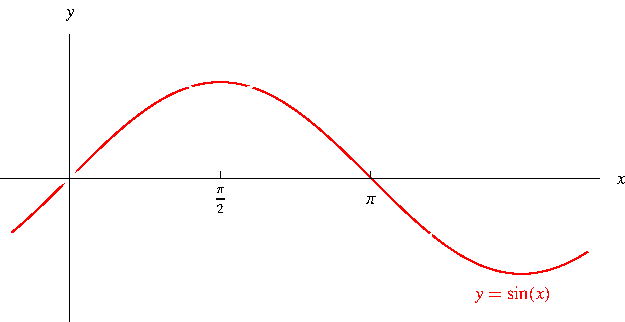
\includegraphics[height=6cm]{precalculus/pictures/01-03-stretcha.pdf}%
%}%
%\only<handout:0| 3>{%
%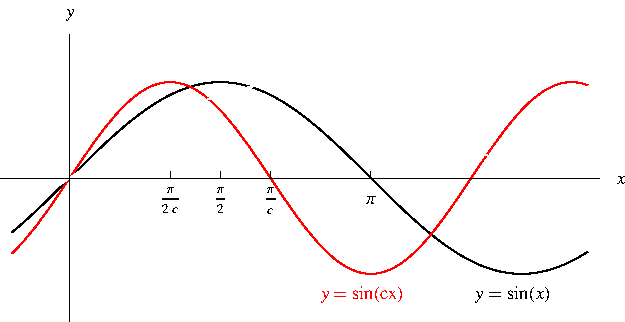
\includegraphics[height=6cm]{precalculus/pictures/01-03-stretchb.pdf}%
%}%
%\only<4->{%
%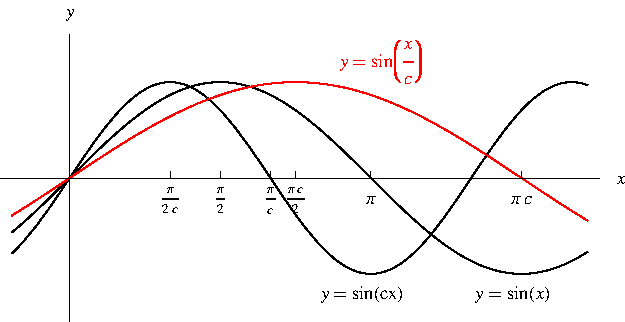
\includegraphics[height=6cm]{precalculus/pictures/01-03-stretchc.pdf}%
%}%a

What happens if we multiply or divide $x$ by a constant $c > 1$ before applying $f$?

\uncover<2->{
\begin{tabular}{|l|l|}
\hline
\alert<handout:0| 3>{$f(cx)$} &%
\uncover<3->{\alert<handout:0| 3>{Compress the graph of $f(x)$ horizontally by a factor of $c$.}} \\%
\alert<handout:0| 4>{$f((1/c)x)$} &%
\uncover<4->{\alert<handout:0| 4>{Stretch the graph of $f(x)$ horizontally by a factor of $c$.}} \\%
\hline
\end{tabular}
}
\end{frame}
% end module transformations-horizontal-stretches

%\begin{frame}
\begin{example}
Let $\alertNoH{2,4}{ f{}({\alertNoH{3,5}{x}})=\alertNoH{3,5}{x}^2- \alertNoH{3,5}{x}-1}$.  Evaluate the difference quotient and \alertNoH{6,13}{simplify your answer}. 
\[
\begin{array}{rcl}
\displaystyle \frac{\alertNoH{2}{ f{}(\alertNoH{3}{2+h})} - \alertNoH{4}{f{}(\alertNoH{4}{2})} }{h}&=&\displaystyle \uncover<2->{\frac{\left( \alertNoH{2}{ \alertNoH{6,7}{ (\alertNoH{3}{2+h})^2} \alertNoH{8}{-}(\alertNoH{3}{2+h})-1} \right) \alertNoH{9}{-} (\alertNoH{4}{\alertNoH{5}{2}^2 \alertNoH{9}{-}\alertNoH{5}{2}\alertNoH{9}{-} 1})}{h}}\\
\uncover<6->{ &=&\displaystyle \frac{ \fcAnswer{7}{\fcCancel{10}{ 2^2} + \alertNoH{11}{2\cdot 2 h} +h^2} \alertNoH{8}{-}\fcCancel{10}{2} \alertNoH{11}{\alertNoH{8}{-}h}-\fcCancel{10}{1} \alertNoH{9}{-} \fcCancel{10}{2^2} \alertNoH{9}{+} \fcCancel{10}{2} \alertNoH{9}{+}\fcCancel{10}{1}}{h} }\\
\uncover<11->{&=&\displaystyle \frac{h^2 + \alertNoH{11}{3h} }{h}}\\
\uncover<12->{&=&\displaystyle \frac{\fcCancel{13}{h}(h+3)}{\fcCancel{13}{h}}}\\
\uncover<13->{&=&\displaystyle h+3}\\
\end{array}
\]


\end{example}
\end{frame}

%\begin{frame}
\vskip -0.15cm
\begin{definition}
Two lines are parallel if they have no common point.
\end{definition}
\vskip -0.15cm
\begin{proposition}
Two non-vertical lines are parallel if and only if they have equal slopes and different $y$ intercepts.
\end{proposition}
\vskip -0.15cm
\begin{proof}[\only<handout:1|1>{Proof $\Leftarrow$}\only<handout:2|2>{Proof $\Rightarrow$} ]
\only<handout:1|1>{
\begin{itemize}
\item Suppose the two lines have different $y$ intercepts and have the same slope $m$.
\item Then the lines have equations as shown below.
\[
\left|\begin{array}{rcl}
y&=& mx+b_1\\
y&=& mx+b_2
\end{array}\right.
\]
\item System has no solutions as $b_1\neq b_2$ $\Rightarrow$ the lines don't intersect.
\end{itemize}
}
\only<handout:2|2->{
\begin{itemize}
\item Suppose the two lines have different slopes. 
\item Suppose the lines have equations as shown below.
$
\begin{array}{c@{}r@{}c@{}l@{}l|l}
&y&=&m_1x+b_1\\
\cline{1-1}&y&=&m_2x+b_2\\\cline{1-4}
&0&=&(m_1-m_2)x+b_1-b_2\\
&(m_1-m_2)x&=&b_2-b_1 &&\text{Div. by }{m_1-m_2\neq 0}\\
&x&=&\displaystyle \frac{b_2-b_1}{m_1-m_2}
\end{array}
$
\item The system has solution $x=  \frac{b_2-b_1}{m_1-m_2}$, $y= m_1\frac{b_2-b_1}{m_1-m_2}+b_1$ $\Rightarrow$ the lines intersect.
\end{itemize}
}
\vskip -0.7cm
\end{proof}

\vskip 10cm

\end{frame}
%\begin{frame}

\begin{definition}
The zeroes of a function $f$ are the values of the argument $x$ for which $f(x)=0$.
\end{definition}

\begin{observation}
The zeroes of a function are the $x$-coordinates of the $x$ intercepts of the graph of the function.
\end{observation}

\begin{pspicture}(-1.2,-1.2)(1.2,1.1)
\fcAxesStandard{-1.2}{-1.2}{1.2}{1.2}
\psplot[linecolor=\fcColorGraph]{-1.2}{1.2}{x 1 sub x x 1 add mul mul}
\fcFullDot{0}{0}
\fcFullDot{1}{0}
\fcFullDot{-1}{0}
\end{pspicture}


\end{frame}
%\begin{frame}

\begin{example}
\begin{columns}
\column{0.45\textwidth}
\begin{pspicture}(-1,-1)(1,1)
\fcAxesStandard{-3.2}{-2}{2.2}{2}
\psplot[linecolor=\fcColorGraph]{-3.2}{2.2}{1 6 div x x x mul mul mul 1 6 div x x mul mul -1 x mul add add }
\uncover<2->{
\fcFullDot{-3}{0}
\fcFullDot{2}{0}
\fcFullDot{0}{0}
}
\end{pspicture}
\column{0.55\textwidth}
Find the zeroes of $\displaystyle  f(x)=\frac{1}{6}x^3+\frac{1}{6}x^2-x$.

\end{columns}
\uncover<2->{}
\end{example}
\end{frame}
%\begin{frame}
Let $g$ of $x$ and $f$ of $x$ be functions.
\begin{columns}

\column{0.45\textwidth}
\psset{xunit=0.5cm, yunit=0.5cm}
\begin{pspicture}(-4,-4)(2.2,3)
\tiny
\fcAxesStandard{-4}{-4}{2.2}{3}
\uncover<2->{
\psplot[linecolor=\fcColorGraph]{-3.2}{2.2}{1 6 div x x x mul mul mul 1 6 div x x mul mul add }
\rput[l](-2,1){$f(x)=\frac{1}{6}x^3+\frac{1}{6}x^2$}
}
\uncover<3->{
\psline[linecolor=\fcColorGraph](-3.2,-3.2)(2.2,2.2)
\rput[t](-1,-2){$g(x)=x$}
}
\uncover<4->{
\fcFullDot{-3}{-3}
\fcFullDot{0}{0}
\fcFullDot{2}{2}
}
\uncover<5->{
\rput[l](-3,-3){$~~(\alertNoH{5,10}{-3}, -3)$}
\rput[tl](0,-0.1){$~~(\alertNoH{5,10}{0}, 0)$}
\rput[r](2,2){$(\alertNoH{5,10}{2}, 2)~~$}
}
\end{pspicture}
\psset{xunit=0.5cm, yunit=0.5cm}
\begin{pspicture}(-4,-4)(2.2,3)
\tiny
\fcAxesStandard{-4}{-4}{2.2}{3}
\uncover<8->{
\psplot[linecolor=\fcColorGraph]{-3.2}{2.2}{1 6 div x x x mul mul mul 1 6 div x x mul mul add -1 x mul add}
}
\uncover<7->{%
\rput(-1,2){$f(x)-g(x)=\frac{1}{6}x^3+\frac{1}{6}x^2-x$}
}%
\uncover<9->{
\fcFullDot{-3}{0}
\fcFullDot{2}{0}
\fcFullDot{0}{0}
}
\uncover<10->{
\rput[tl](-3, -0.1){$(\alertNoH{10}{-3},0)$}
\rput[tl](0, -0.1){$~~(\alertNoH{10}{0},0)$}
\rput[br](2, 0.1){$(\alertNoH{10}{2},0)~~$}
}
\end{pspicture}
\column{0.55\textwidth}
\begin{observation}
\begin{itemize}
\item To solve $\alertNoH{2}{f(x)}=\alertNoH{3}{g(x)}$ means to find the \alertNoH{5}{$x$ coordinates} of the \alertNoH{4}{intersections of the graphs of $f$ and $g$}. 
\item<6-> To solve $f(x)=g(x)$ is equivalent to solving the equation $f(x)-g(x)=0$.
\item<7-> To solve $f(x)=g(x) $ means to find \alertNoH{9}{the zeroes} of $\alertNoH{7,8}{f(x)-g(x)}$.
\item<10-> The \alertNoH{10}{$x$ coordinates of the intersections of $f(x)$ and $g(x)$} coincide with the \alertNoH{10}{$x$ coordinates of the $x$ intercepts of $f(x)-g(x)$}.
\end{itemize}
\end{observation}
\end{columns}
\end{frame}
%\begin{frame}
\begin{example}
\begin{itemize}
\item Find when $f(x)=g(x)$, where 
\[
f(x)=\frac{1}{6}x^3+\frac{1}{6}x^2\qquad \qquad g(x)=x
\]
\item Find the intersections of the graphs of $f$ and $g$.
\end{itemize}
\end{example}
\end{frame}

%\begin{frame}
\begin{definition}[Completing the square]
Let $a\neq 0$. \alertNoH{13}{To \emph{complete the square} means} to carry out the following algebraic manipulation.
$
\begin{array}{@{\!\!}r@{}c@{}l@{}l|l}
\displaystyle \alertNoH{13}{ \alertNoH{2}{ax^2}+\alertNoH{3}{b} x+c } \uncover<2->{&\alertNoH{0}{=}&\displaystyle  \alertNoH{2,3}{a}\left( \alertNoH{2}{x^2}+ \alertNoH{3}{\frac{b}{a}}x \right)+c }\\
\uncover<4->{&\alertNoH{0}{=}&\displaystyle  a\! \left(x^{2}+\alertNoH{4}{2}\cdot \alertNoH{6}{\frac{b}{\alertNoH{4}{2}a}} x \right) +c}\\
\uncover<5->{&\alertNoH{0}{=}&\displaystyle  a\left( \! \alertNoH{7}{\alertNoH{8}{x}^{2}+2\alertNoH{6,9}{ \frac{ b }{ 2 a}} \alertNoH{8}{x} \alertNoH{5}{+{\left( \uncover<6->{\alertNoH{6, 9}{\frac{ b}{2a}}}\right)}^2}}\! \!\alertNoH{5}{- \alertNoH{10}{{\left( \uncover<6->{\alertNoH{6}{\frac{ b}{2 a}}}\right)}^2}} \right)+c} \uncover<5->{&& \begin{array}{@{}l} \text{\alertNoH{5}{Add \& subtract}} \\ {\left( \uncover<6->{\alertNoH{6}{ \frac{ b}{2a}}}\right)}^2\end{array}} \\
\uncover<7->{&\alertNoH{0}{=}&\displaystyle \alertNoH{11}{ a} \left( \alertNoH{7}{\left(\alertNoH{8}{x}+ \alertNoH{9}{\frac{ b}{2 a}}\right)^2} -\alertNoH{10}{\frac{b^2}{4a^2}} \right)+c &&\begin{array}{@{}l} \alertNoH{7}{\text{use }}\\ \alertNoH{7}{(\alertNoH{8}{A}+\alertNoH{9}{B})^2=}\\ \alertNoH{7}{\alertNoH{8}{A}^2+2\alertNoH{8}{A}\alertNoH{9}{B}+\alertNoH{9}{B}^2} \end{array}}\\
\uncover<11->{&\alertNoH{0}{=}&\displaystyle  \alertNoH{11}{a} \left(x +\frac{b}{2a}\right)^2 - \fcCancel{12}{\alertNoH{11}{a}} \cdot \frac{b^2}{4a^{\fcCancel{12}{2}}} +c} \\
\uncover<12->{&\alertNoH{13}{=}&\displaystyle  \alertNoH{13}{a\left(x +\frac{ b}{2a}\right)^2 + c-  \frac{b^2}{4a}}.}
\end{array}
$

\end{definition}

\end{frame}

%\begin{frame}
\begin{pspicture}(-1, -1)(2,2)
\fcBoundingBox{-3}{-3}{4}{4} %
\fcStartIIIdScene%
\fcSurfaceInScene[iterationsU=33, iterationsV=5]{0}{-1}{360}{1}{%
[10 dict begin
/R 2 def
/r {0.6 v mul} def
/theta u def
/phi {u 0.5 mul} def
/A {phi cos r mul R add} def
theta cos A mul theta sin A mul phi sin r mul
end %
]%
}{}%
\fcSurfaceInScene[iterationsU=33, iterationsV=5, colorUV=cyan, colorVU=blue]{0}{-1}{360}{1}{%
[[0 0 1] [0 1 0] [1 0 0] ]
[10 dict begin
/R 2 def
/r {0.6 v mul} def
/theta u def
/phi {u 0.5 mul} def
/A {phi cos r mul R add} def
theta cos A mul theta sin A mul phi sin r mul
end %
] \fcMatrixTimesVector [-1.1 -1.1 0] \fcVectorPlusVector
%
}{}%
%\fcLineIIIdInScene[linewidth=2, linecolor=cyan]{[-1 -1 -1]}{[1 1 1]}
\fcFinishIIIdScene %
%\fcAxesIIId{4}{4}{4}
\end{pspicture}
\end{frame}


%% begin module differentiation-formulas-ex1
\begin{frame}
\alert<1>{You will not be tested on the material in the following slide.}
\end{frame}
\begin{frame}
\frametitle{Derivative ball volume =surface area}
The relationship between surface area and volume of a ball.

\footnotesize
\begin{tabular}{|p{0.7cm}p{2cm}p{1cm}p{1cm}p{1cm}p{1cm}p{2.5cm}|}\hline
\alert<0>{Di-men-sion} & \alert<2,14,26>{Pts. at distance $\leq r$ from origin} &  \alert<4,16,28>{Inside-volume name} & \alert<6, 18,30>{Inside-volume f-la} & \alert<8,20,32>{Boundary name} & \alert<10,22,34>{Boundary area f-la} & \alert<12,24,36>{Derivative inside-volume}\\\hline
%
\alert<2>{3} & \uncover<3->{\alert<3>{ball}} & \uncover<5->{\alert<5>{ball volume}} &  \uncover<7->{\alert<7, 12>{$\frac {4}{3}\pi r^3$}} & \uncover<9->{\alert<9>{sphere surface area} } & \uncover<11->{\alert<11, 13>{$4\pi r^2$}} & \uncover<12->{$\alert<12>{\frac{d}{dr}\left(\frac {4}{3}\pi r^3\right)=}\uncover<13->{\alert<13>{4\pi r^2}}$} \\\hline
%
\alert<14>{2} & \uncover<15->{\alert<15>{disk, circle}} & \uncover<17->{\alert<17>{circle area}} & \uncover<19->{\alert<19,24>{$\pi r^2$}} & \uncover<21->{\alert<21>{circle circum-ference}} & \uncover<23->{\alert<23,25>{$2\pi r$}} & \uncover<24->{${\alert<24>{\frac{d}{dr}\left(\pi r^2\right)=}} \uncover<25->{\alert<25>{2\pi r}}$} \\\hline
%
\alert<26>{1} & \uncover<27->{\alert<27>{interval}} & \uncover<29->{\alert<29>{length}} & \uncover<31->{\alert<31>{$2r$}} & \uncover<33->{\alert<33>{the two endpoints}} & \uncover<35->{\alert<35,37>{$2$}} &\uncover<36->{$\alert<36>{\frac{d}{dr}(2r)=} \uncover<37->{\alert<37>{2}}$} \\
\hline
\end{tabular}
\end{frame}
% end module differentiation-formulas-ex1

%% begin module area-def
\begin{frame}
Estimate the area under the curve $y = f(x)$ between $a$ and $b$.
\begin{columns}
\column{.55\textwidth}
\psset{xunit=3cm, yunit=3cm}
\begin{pspicture}(-5, -5)(5,5)
\psframe*[linecolor=white](-5,-5)(5,5)
\psaxes[ticks=none, labels=none]{<->}(0,0)(-0.1,-0.1)(1.7,0.9)
\tiny

\uncover<1>{
\psline*[linecolor=\fcColorAreaUnderGraph, linewidth=0.1pt](0.425, 0)(0.425, 0.339931)(0.3, 0.339931)(0.3, 0)(0.55, 0)(0.55, 0.316508)(0.425, 0.316508)(0.425, 0)(0.675, 0)(0.675, 0.348456)(0.55, 0.348456)(0.55, 0)(0.8, 0)(0.8, 0.416)(0.675, 0.416)(0.675, 0)(0.925, 0)(0.925, 0.499364)(0.8, 0.499364)(0.8, 0)(1.05, 0)(1.05, 0.578773)(0.925, 0.578773)(0.925, 0)(1.175, 0)(1.175, 0.634452)(1.05, 0.634452)(1.05, 0)(1.3, 0)(1.3, 0.646625)(1.175, 0.646625)(1.175, 0)(1.425, 0)(1.425, 0.595517)(1.3, 0.595517)(1.3, 0)(1.55, 0)(1.55, 0.461352)(1.425, 0.461352)(1.425, 0)
\psline[linecolor=blue, linewidth=0.1pt](0.425, 0)(0.425, 0.339931)(0.3, 0.339931)(0.3, 0)(0.55, 0)(0.55, 0.316508)(0.425, 0.316508)(0.425, 0)(0.675, 0)(0.675, 0.348456)(0.55, 0.348456)(0.55, 0)(0.8, 0)(0.8, 0.416)(0.675, 0.416)(0.675, 0)(0.925, 0)(0.925, 0.499364)(0.8, 0.499364)(0.8, 0)(1.05, 0)(1.05, 0.578773)(0.925, 0.578773)(0.925, 0)(1.175, 0)(1.175, 0.634452)(1.05, 0.634452)(1.05, 0)(1.3, 0)(1.3, 0.646625)(1.175, 0.646625)(1.175, 0)(1.425, 0)(1.425, 0.595517)(1.3, 0.595517)(1.3, 0)(1.55, 0)(1.55, 0.461352)(1.425, 0.461352)(1.425, 0)
}
\uncover<2->{
\psline*[linecolor=\fcColorAreaUnderGraph, linewidth=0.1pt](0.3, 0)(0.3, 0.4385)(0.425, 0.4385)(0.425, 0)(0.425, 0)(0.425, 0.339931)(0.55, 0.339931)(0.55, 0)(0.55, 0)(0.55, 0.316508)(0.675, 0.316508)(0.675, 0)(0.675, 0)(0.675, 0.348456)(0.8, 0.348456)(0.8, 0)(0.8, 0)(0.8, 0.416)(0.925, 0.416)(0.925, 0)(0.925, 0)(0.925, 0.499364)(1.05, 0.499364)(1.05, 0)(1.05, 0)(1.05, 0.578773)(1.175, 0.578773)(1.175, 0)(1.175, 0)(1.175, 0.634452)(1.3, 0.634452)(1.3, 0)(1.3, 0)(1.3, 0.646625)(1.425, 0.646625)(1.425, 0)(1.425, 0)(1.425, 0.595517)(1.55, 0.595517)(1.55, 0)
\psline[linecolor=blue, linewidth=0.1pt](0.3, 0)(0.3, 0.4385)(0.425, 0.4385)(0.425, 0)(0.425, 0)(0.425, 0.339931)(0.55, 0.339931)(0.55, 0)(0.55, 0)(0.55, 0.316508)(0.675, 0.316508)(0.675, 0)(0.675, 0)(0.675, 0.348456)(0.8, 0.348456)(0.8, 0)(0.8, 0)(0.8, 0.416)(0.925, 0.416)(0.925, 0)(0.925, 0)(0.925, 0.499364)(1.05, 0.499364)(1.05, 0)(1.05, 0)(1.05, 0.578773)(1.175, 0.578773)(1.175, 0)(1.175, 0)(1.175, 0.634452)(1.3, 0.634452)(1.3, 0)(1.3, 0)(1.3, 0.646625)(1.425, 0.646625)(1.425, 0)(1.425, 0)(1.425, 0.595517)(1.55, 0.595517)(1.55, 0)
}
\rput[t](0.3,-0.03){$a$}
\rput[t](0.425,-0.03){$x_1$}
\rput[t](0.55,-0.03){$x_2$}
%\rput[t](0.675,-0.03){}
%\rput[t](0.8,-0.03){$\frac{4}{5}$}
\rput[t](0.7375,-0.06){$\dots$}
\rput[t](0.925,-0.03){$x_{i-1}$}
\rput[t](1.05,-0.03){$x_{i}$}
%\rput[t](1.175,-0.03){$x_i$}
%\rput[t](1.3,-0.03){$\frac{13}{10}$}
\rput[t](1.3,-0.06){$\dots$}
%\rput[t](1.425,-0.03){$\frac{57}{40}$}
\rput[t](1.55,-0.03){$b$}
%Function formula: -171/50 (x)-27/16 ((x)^{3})+11/10+729/160 ((x)^{2})
\psplot[linecolor=red, plotpoints=1000]{0.3}{1.55}{x 2 exp 4.55625 mul 1.1 add x 3 exp -1.6875 mul add x -3.42 mul add }
\psline{<->}(1.6,0)(1.6, 0.578773)
\psline[linestyle=dotted](1.6, 0.578773)(1.05, 0.578773)
\rput[l](1.6, 0.3343865){$f(x_i)$}
\rput[b](0.9875,0.70773){$\Delta x$}
\psline(0.925,0.668773)(1.05, 0.668773)
\psline(0.925,0.648773)(0.925,0.688773)
\psline(1.05, 0.648773)(1.05, 0.688773)

%\psbrace[linecolor=red,ref=lC](2)(3){Text I}
%\uput{:U}{$\overbrace{}^\text{\normalsize A line}$}
\end{pspicture}
%\only<handout:1| -1>{%
%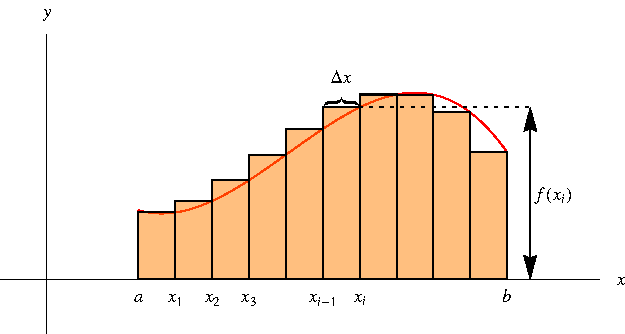
\includegraphics[height=3.5cm]{integration/pictures/05-01-rectangles-right.pdf}%
%}%
%\only<handout:2| 2->{%
%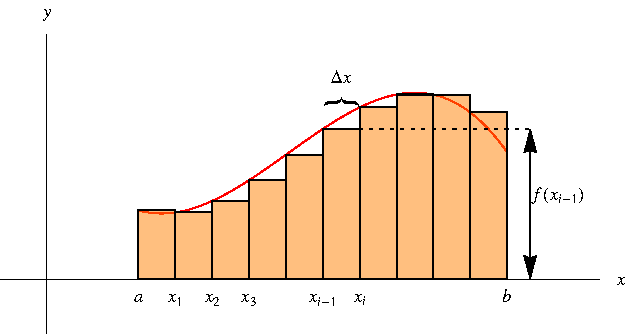
\includegraphics[height=3.5cm]{integration/pictures/05-01-rectangles-left.pdf}%
%}%



\begin{itemize}
\item<1->  The width of the interval is $b-a$.
\item<1->  The width of each of the $n$ strips is $\Delta x = \frac{b-a}{n}$.
\item<1->  The strips divide $[a,b]$ into $n$ subintervals:\\ $[x_0, x_1]$, $[x_1,x_2]$, $\ldots ,$ $[x_{n-1},x_n]$,\\ where $x_0 = a$ and $x_n = b$.
\end{itemize}
\column{.45\textwidth}
\begin{itemize}
\item<1->  The \only<handout:1| -1>{right}\only<handout:2| 2->{\alert<handout:2| 2>{left}} endpoints of the subintervals are
\end{itemize}
\abovedisplayskip=0pt
\belowdisplayskip=0pt
\begin{eqnarray*}
x_{\only<handout:1| -1>{1}\only<handout:2| 2->{\alert<handout:2| 2>{0}}} & = & a \only<handout:1| -1>{+ \Delta x}\\
x_{\only<handout:1| -1>{2}\only<handout:2| 2->{\alert<handout:2| 2>{1}}} & = & a + \only<handout:1| -1>{2}\Delta x\\
x_{\only<handout:1| -1>{3}\only<handout:2| 2->{\alert<handout:2| 2>{2}}} & = & a + \only<handout:1| -1>{3}\only<handout:2| 2->{2}\Delta x\\
& \vdots &
\end{eqnarray*}
\begin{itemize}
\item<1->  The height of the $i$th rectangle is $f(x_{i\only<handout:2| 2->{\alert<handout:2| 2>{-1}}})$.
\item<1->  The area of the $i$th rectangle is $f(x_{i\only<handout:2| 2->{\alert<handout:2| 2>{-1}}})\Delta x$.
\end{itemize}
\end{columns}
\abovedisplayskip=0pt
\belowdisplayskip=0pt
\[
\only<handout:1| -1>{R_n}\only<handout:2| 2->{\alert<handout:2| 2>{L_n}} = f(x_{\only<handout:1| -1>{1}\only<handout:2| 2->{\alert<handout:2| 2>{0}}})\Delta x + f(x_{\only<handout:1| -1>{2}\only<handout:2| 2->{\alert<handout:2| 2>{1}}})\Delta x + f(x_{\only<handout:1| -1>{3}\only<handout:2| 2->{\alert<handout:2| 2>{2}}})\Delta x + \cdots + f(x_{n\only<handout:2| 2->{\alert<handout:2| 2>{-1}}})\Delta x
\]
\end{frame}

\begin{frame}
\begin{definition}[Area Under a Curve]
The area of the region $S$ that lies under the curve $y = f(x)$ is the limit of the sum of the areas of the approximating rectangles:
\abovedisplayskip=0pt
\belowdisplayskip=0pt
\[
A = \lim_{n\to\infty} R_n = \lim_{n\to\infty} [ f(x_1)\Delta x + f(x_2) \Delta x + \cdots + f(x_n) \Delta x]
\]
\end{definition}
\begin{itemize}
\item<2->  This limit always exists if $f$ is continuous.
\item<3->  If $f$ is continuous, we get the same limit if we use left endpoints:
\abovedisplayskip=0pt
\belowdisplayskip=0pt
\[
A = \lim_{n\to\infty} L_n = \lim_{n\to\infty} [ f(x_0)\Delta x + f(x_1) \Delta x + \cdots + f(x_{n-1}) \Delta x]
\]
\item<4->  If $f$ is continuous, we get the same limit if we use any number $x_i^*$ in the interval $[x_{i-1},x_i]$.  $x_i^*$ is called a sample point.
\abovedisplayskip=0pt
\belowdisplayskip=0pt
\[
A = \lim_{n\to\infty} [ f(x_1^*)\Delta x + f(x_2^*) \Delta x + \cdots + f(x_{n}^*) \Delta x]
\]
\end{itemize}
\uncover<5->{%
\begin{definition}[Riemann Sum]
A Riemann sum is any sum of the form
\abovedisplayskip=0pt
\belowdisplayskip=0pt
\[
f(x_1^*)\Delta x + f(x_2^*) \Delta x + \cdots + f(x_{n}^*) \Delta x.
\]
\end{definition}
}%
\end{frame}
% end module area-def

%% begin module sigma-notation
\begin{frame}
\[
\mathop{\alert<handout:0| 2>{\sum}}_{\alert<handout:0| 3>{i=1}}^{\alert<handout:0| 4>{n}} f(x_i)\Delta x = f(x_1)\Delta x + f(x_2)\Delta x + \cdots + f(x_n)\Delta x
\]
\begin{itemize}
\item  We use sigma notation to write sums more compactly.
\item<2-| alert@2>  $\sum$ is the Greek letter sigma.  It tells us to add.
\item<3-| alert@3>  The subscript tells us to start at 1.
\item<4-| alert@4>  The superscript tells us to finish at $n$.
\end{itemize}
\uncover<5->{%
\begin{example}
\begin{eqnarray*}
\sum_{i=1}^4 2i\Delta x & = & 2\Delta x + 4 \Delta x + 6 \Delta x + 8\Delta x\\
\uncover<6->{\alert<handout:0| 6-7>{\sum_{i=3}^7 i^2\Delta x}} & \uncover<6->{\alert<handout:0| 6-7>{=}} & \uncover<7->{\alert<handout:0| 7>{9\Delta x + 16 \Delta x + 25 \Delta x + 36\Delta x + 49\Delta x}}
\end{eqnarray*}
\end{example}
}%
\end{frame}
% end module sigma-notation

%\begin{frame}
\vskip -0.1cm
\begin{example}[The $\dots$ and $\sum$ notations for series]
Let \alertNoH{3,4}{$A$ be the sum of the positive even integers between 2 and and 124}. \uncover<2->{Write $A$ \alertNoH{3,4}{using the $\dots$ notation} and using the $\sum$ notation.}

\vskip -0.2cm
\[
\begin{array}{rcl}
\uncover<3->{\alertNoH{3,4}{A}&\alertNoH{3,4}{=}&\displaystyle \fcAnswer{4}{\alertNoH{6,27}{2+4+6+\dots+\alertNoH{28}{124}}}} \\
\uncover<7->{&=& \alertNoH{9}{2} + \alertNoH{10}{4}+\alertNoH{11}{6}+\dots + \alertNoH{7,8,12}{2n}+\dots +\alertNoH{ 13}{124}} \\
\uncover<9->{&=& \alertNoH{9,17}{2\cdot \alertNoH{18,19,21}{ 1}} +\alertNoH{10,17}{2\cdot \alertNoH{18,22}{2} }+\alertNoH{11,17}{2\cdot \alertNoH{18,23}{3}}+ \dots+\alertNoH{12,17}{ 2\cdot \alertNoH{18,24}{n} }+\dots +\alertNoH{13,17}{2\cdot \alertNoH{ 18,20,25 }{62} } } \\
\uncover<8->{&\uncover<14->{=}& \displaystyle  \uncover<14->{ \only<handout:0 | 16>{\color{red}} \sum \limits_{ {\color{black}  \alertNoH{15}{n} =\alertNoH{19,21}{1} }}^{ {\color{black} \alertNoH{20,25,28}{62}}} }\color{black} \alertNoH{8-13,17, 27,28}{ 2 \alertNoH{15,18,21-25}{n}} \quad .} 
\end{array}
\]

\end{example}
\begin{itemize}
\only<handout:1|1-14>{ 
\item<5-> We aim to introduce the $\sum $ notation for series via this example.

\item<6-> The $\dots$ notation is informal but easier to read.
\item<7-> If the $\dots $ are too ambiguous, we should include the general term.
\item<8-> To make it clearer we should rewrite all elements in the \alertNoH{8-12}{pattern of the general term}.
\item<14-> If that is still ambiguous we should switch to the completely unambiguous $\sum$ notation. 
}
\only<handout:2|15-26>{
\item<15-> The number $\alertNoH{14}{n}$ is the \alertNoH{14}{index (counter)} of the sum.
\item<16-> \alertNoH{16}{$\sum$ tells us to add} \alertNoH{17}{several copies of the summed term}, \alertNoH{18}{where in each term the index is replaced by a concrete value}.
\item<19-> The values taken by the index are determined by the \alertNoH{19,20}{boundaries of summation}. 
\item<21-> The index varies over all integers starting with the lower boundary and ending with upper boundary. 
\item<26-> In programming, what objects are similar to $\sum$?
}
\only<handout:3|27-29>{
\item<27-> To go from $\sum$ to $\dots$ notation: substitute few values for the index. \alertNoH{28}{Make sure to include the last value.}
\item<28-> To go from $\dots$ to $\sum $ notation: 
\begin{itemize}
\item<28-> figure out a pattern for the general term just as with sequences;
\item<29-> select first and last index so that your general term formula reproduces the first and last terms of the sequence.
\end{itemize}
}
\only<handout:4|30->{
\item Bear in mind the $\dots$ notation is informal. 
\begin{itemize}
\item<31-> There are infinitely many formulas that fit any single pattern.
\item<32-> Thus it is acceptable to use the $\dots$ notation only when we believe there is a single completely obvious pattern that will be recognized by every one.
\item<33-> The pattern should be obvious not only to us, but also to our potential readers.
\item<34-> If in doubt or seeking complete rigor we should use the $\sum$ notation. 
\end{itemize}  

}
\end{itemize}

\vskip 4cm
\end{frame}

%% begin module definite-integral-def
\begin{frame}\frametitle{ %(5.2) 
The Definite Integral}
\begin{definition}[Definite Integral]
\begin{itemize}
\item  Let $f$ be a function defined for $a\leq x\leq b$.
\item  Divide the interval $[a,b]$ into $n$ subintervals of equal width $\Delta x = (b-a)/n$ nd set $x_0=a$, $x_n=b$.
\item  Let $x_0$, $x_1,\ldots ,$ $x_n $ be the endpoints of the subintervals.
\item  Let $x_1^*, x_2^*, \ldots , x_n^*$ be any sample points in these subintervals; that is, $x_i^*$ is in $[x_{i-1},x_i]$.  
\end{itemize}
\abovedisplayskip=0pt
\belowdisplayskip=0pt
Suppose the limit $\lim\limits_{n\to \infty} \sum\limits_{i=1}^n f(x_i^*)\Delta x$ exists and is independent of the choice of sample points $x_i^*$. Then we call this limit the integral of $f$ over $[a,b]$ and write
\[
\int_a^b f(x) \diff x = \lim_{n\to \infty} \sum_{i=1}^n f(x_i^*)\Delta x \quad .
\]
\end{definition}
\end{frame}

\begin{frame}
\[
\mathop{\alert<handout:0| 2>{\int}}_{\alert<handout:0| 4>{a}}^{\alert<handout:0| 4>{b}} \alert<handout:0| 3>{f(x)} \alert<handout:0| 0>{\diff x} = \lim_{n\to \infty} \sum_{i=1}^n f(x_i^*)\Delta x,
\]
\begin{itemize}
\item<1-| alert@2>  $\int$ is called the integration sign.
\item<1-| alert@3>  $f(x)$ is called the integrand.
\item<1-| alert@4>  $a$ and $b$ are called the limits of integration.
\item<5->  The definite integral is a number.  It does not depend on $x$.  We could use any variable instead of $x$.
\end{itemize}
\uncover<5->{%
\[
\int_a^b f(x) \diff x = \int_a^b f(t)\diff t = \int_a^b f(r)\diff r = \int_a^b f(\theta )\diff \theta
\]
}%
\end{frame}
% end module definite-integral-def

%% begin module continuous-functions-integrable
\begin{frame}
\begin{theorem}
Let $f$ be a continuous function on $[a,b]$. Then $f$ is integrable over $[a,b]$.
\end{theorem}
\begin{itemize}
\item In particular the integral does not depend the choice of sampling points so long as the intervals containing them shrink.
\item The proof of this theorem is not difficult, but is outside of the scope of Calculus I and II.
\item The only ``difficulty'' in the proof stems from the fact that we have not rigorously constructed the real numbers. 
\item We already (silently) assumed a construction of the real numbers when we defined limits. 
\item Such a construction is also (silently) assumed in most regular high school mathematics courses.
%\item  The proof of the Theorem uses the fact that every set bounded above has a least upper bound. The latter fact is either taken as an axiom of the real numbers, or is proven from equivalent set of axioms. This is the main fact a calculus student is missing to understand/prove on one's own the above theorem.
\item A student interested in a proof of the theorem should google ``Darboux integral''.
\end{itemize}

\end{frame}
% end module continuous-functions-integrable

%% begin module definite-integral-negative
\begin{frame}
\begin{columns}
\column{.55\textwidth}
\begin{itemize}
\item  We know already that if $f(x)$ is always positive, then $\int_a^bf(x)\diff x$ is the area under the curve.
\end{itemize}
\column{.45\textwidth}
\psset{xunit=2cm, yunit=2cm}
\begin{pspicture}(-0.15,-0.15)(1.5,1.5)
\psline{linecolor=red!1}(0, -0.3)(0, -0.31)
\psframe*[linecolor=white](-0.15,-0.15)(1.5,1.5)
\tiny
\psline(-0.05, 1)(0.05,1)
\rput[r] (-0.07,1){$1$}
%Function formula: x^{2}
\rput(0.9,1.3){$y=x^{2}$}
\uncover<handout:0|1>{
%approximation 1/3
\psline*[linecolor=\fcColorAreaUnderGraph, linewidth=0.1pt](0.333333, 0)(0.333333, 0.111111)(0, 0.111111)(0, 0)(0.666667, 0)(0.666667, 0.444444)(0.333333, 0.444444)(0.333333, 0)(1, 0)(1, 1)(0.666667, 1)(0.666667, 0)
\psline[linecolor=blue, linewidth=0.1pt](0.333333, 0)(0.333333, 0.111111)(0, 0.111111)(0, 0)(0.666667, 0)(0.666667, 0.444444)(0.333333, 0.444444)(0.333333, 0)(1, 0)(1, 1)(0.666667, 1)(0.666667, 0)
\rput[t](0.333333,-0.03){$\frac{1}{3}$}\rput[t](0.666667,-0.03){$\frac{2}{3}$}\rput[t](1,-0.03){$1$}
}
\uncover<handout:0|2>{
%approximation 1/4
\psline*[linecolor=\fcColorAreaUnderGraph, linewidth=0.1pt](0.25, 0)(0.25, 0.0625)(0, 0.0625)(0, 0)(0.5, 0)(0.5, 0.25)(0.25, 0.25)(0.25, 0)(0.75, 0)(0.75, 0.5625)(0.5, 0.5625)(0.5, 0)(1, 0)(1, 1)(0.75, 1)(0.75, 0)
\psline[linecolor=blue, linewidth=0.1pt](0.25, 0)(0.25, 0.0625)(0, 0.0625)(0, 0)(0.5, 0)(0.5, 0.25)(0.25, 0.25)(0.25, 0)(0.75, 0)(0.75, 0.5625)(0.5, 0.5625)(0.5, 0)(1, 0)(1, 1)(0.75, 1)(0.75, 0)
\rput[t](0.25,-0.03){$\frac{1}{4}$}\rput[t](0.5,-0.03){$\frac{1}{2}$}\rput[t](0.75,-0.03){$\frac{3}{4}$}\rput[t](1,-0.03){$1$}
}
\uncover<handout:0|3>{
%approximation 1/5
\psline*[linecolor=\fcColorAreaUnderGraph, linewidth=0.1pt](0.2, 0)(0.2, 0.04)(0, 0.04)(0, 0)(0.4, 0)(0.4, 0.16)(0.2, 0.16)(0.2, 0)(0.6, 0)(0.6, 0.36)(0.4, 0.36)(0.4, 0)(0.8, 0)(0.8, 0.64)(0.6, 0.64)(0.6, 0)(1, 0)(1, 1)(0.8, 1)(0.8, 0)
\psline[linecolor=blue, linewidth=0.1pt](0.2, 0)(0.2, 0.04)(0, 0.04)(0, 0)(0.4, 0)(0.4, 0.16)(0.2, 0.16)(0.2, 0)(0.6, 0)(0.6, 0.36)(0.4, 0.36)(0.4, 0)(0.8, 0)(0.8, 0.64)(0.6, 0.64)(0.6, 0)(1, 0)(1, 1)(0.8, 1)(0.8, 0)
\rput[t](0.2,-0.03){$\frac{1}{5}$}\rput[t](0.4,-0.03){$\frac{2}{5}$}\rput[t](0.6,-0.03){$\frac{3}{5}$}\rput[t](0.8,-0.03){$\frac{4}{5}$}\rput[t](1,-0.03){$1$}
}
\uncover<handout:0|4>{
%approximation 1/8
\psline*[linecolor=\fcColorAreaUnderGraph, linewidth=0.1pt](0.125, 0)(0.125, 0.015625)(0, 0.015625)(0, 0)(0.25, 0)(0.25, 0.0625)(0.125, 0.0625)(0.125, 0)(0.375, 0)(0.375, 0.140625)(0.25, 0.140625)(0.25, 0)(0.5, 0)(0.5, 0.25)(0.375, 0.25)(0.375, 0)(0.625, 0)(0.625, 0.390625)(0.5, 0.390625)(0.5, 0)(0.75, 0)(0.75, 0.5625)(0.625, 0.5625)(0.625, 0)(0.875, 0)(0.875, 0.765625)(0.75, 0.765625)(0.75, 0)(1, 0)(1, 1)(0.875, 1)(0.875, 0)
\psline[linecolor=blue, linewidth=0.1pt](0.125, 0)(0.125, 0.015625)(0, 0.015625)(0, 0)(0.25, 0)(0.25, 0.0625)(0.125, 0.0625)(0.125, 0)(0.375, 0)(0.375, 0.140625)(0.25, 0.140625)(0.25, 0)(0.5, 0)(0.5, 0.25)(0.375, 0.25)(0.375, 0)(0.625, 0)(0.625, 0.390625)(0.5, 0.390625)(0.5, 0)(0.75, 0)(0.75, 0.5625)(0.625, 0.5625)(0.625, 0)(0.875, 0)(0.875, 0.765625)(0.75, 0.765625)(0.75, 0)(1, 0)(1, 1)(0.875, 1)(0.875, 0)
\rput[t](0.125,-0.03){$\frac{1}{8}$}\rput[t](0.25,-0.03){$\frac{1}{4}$}\rput[t](0.375,-0.03){$\frac{3}{8}$}\rput[t](0.5,-0.03){$\frac{1}{2}$}\rput[t](0.625,-0.03){$\frac{5}{8}$}\rput[t](0.75,-0.03){$\frac{3}{4}$}\rput[t](0.875,-0.03){$\frac{7}{8}$}\rput[t](1,-0.03){$1$}
}
\uncover<handout:0|5>{
%approximation 1/10
\psline*[linecolor=\fcColorAreaUnderGraph, linewidth=0.1pt](0.1, 0)(0.1, 0.01)(0, 0.01)(0, 0)(0.2, 0)(0.2, 0.04)(0.1, 0.04)(0.1, 0)(0.3, 0)(0.3, 0.09)(0.2, 0.09)(0.2, 0)(0.4, 0)(0.4, 0.16)(0.3, 0.16)(0.3, 0)(0.5, 0)(0.5, 0.25)(0.4, 0.25)(0.4, 0)(0.6, 0)(0.6, 0.36)(0.5, 0.36)(0.5, 0)(0.7, 0)(0.7, 0.49)(0.6, 0.49)(0.6, 0)(0.8, 0)(0.8, 0.64)(0.7, 0.64)(0.7, 0)(0.9, 0)(0.9, 0.81)(0.8, 0.81)(0.8, 0)(1, 0)(1, 1)(0.9, 1)(0.9, 0)
\psline[linecolor=blue, linewidth=0.1pt](0.1, 0)(0.1, 0.01)(0, 0.01)(0, 0)(0.2, 0)(0.2, 0.04)(0.1, 0.04)(0.1, 0)(0.3, 0)(0.3, 0.09)(0.2, 0.09)(0.2, 0)(0.4, 0)(0.4, 0.16)(0.3, 0.16)(0.3, 0)(0.5, 0)(0.5, 0.25)(0.4, 0.25)(0.4, 0)(0.6, 0)(0.6, 0.36)(0.5, 0.36)(0.5, 0)(0.7, 0)(0.7, 0.49)(0.6, 0.49)(0.6, 0)(0.8, 0)(0.8, 0.64)(0.7, 0.64)(0.7, 0)(0.9, 0)(0.9, 0.81)(0.8, 0.81)(0.8, 0)(1, 0)(1, 1)(0.9, 1)(0.9, 0)
\rput[t](0.1,-0.03){$\frac{1}{10}$}\rput[t](0.2,-0.03){$\frac{1}{5}$}\rput[t](0.3,-0.03){$\frac{3}{10}$}\rput[t](0.4,-0.03){$\frac{2}{5}$}\rput[t](0.5,-0.03){$\frac{1}{2}$}\rput[t](0.6,-0.03){$\frac{3}{5}$}\rput[t](0.7,-0.03){$\frac{7}{10}$}\rput[t](0.8,-0.03){$\frac{4}{5}$}\rput[t](0.9,-0.03){$\frac{9}{10}$}\rput[t](1,-0.03){$1$}
}
\uncover<handout:1|6>{
%approximation 1/20
\psline*[linecolor=\fcColorAreaUnderGraph, linewidth=0.1pt](0.05, 0)(0.05, 0.0025)(0, 0.0025)(0, 0)(0.1, 0)(0.1, 0.01)(0.05, 0.01)(0.05, 0)(0.15, 0)(0.15, 0.0225)(0.1, 0.0225)(0.1, 0)(0.2, 0)(0.2, 0.04)(0.15, 0.04)(0.15, 0)(0.25, 0)(0.25, 0.0625)(0.2, 0.0625)(0.2, 0)(0.3, 0)(0.3, 0.09)(0.25, 0.09)(0.25, 0)(0.35, 0)(0.35, 0.1225)(0.3, 0.1225)(0.3, 0)(0.4, 0)(0.4, 0.16)(0.35, 0.16)(0.35, 0)(0.45, 0)(0.45, 0.2025)(0.4, 0.2025)(0.4, 0)(0.5, 0)(0.5, 0.25)(0.45, 0.25)(0.45, 0)(0.55, 0)(0.55, 0.3025)(0.5, 0.3025)(0.5, 0)(0.6, 0)(0.6, 0.36)(0.55, 0.36)(0.55, 0)(0.65, 0)(0.65, 0.4225)(0.6, 0.4225)(0.6, 0)(0.7, 0)(0.7, 0.49)(0.65, 0.49)(0.65, 0)(0.75, 0)(0.75, 0.5625)(0.7, 0.5625)(0.7, 0)(0.8, 0)(0.8, 0.64)(0.75, 0.64)(0.75, 0)(0.85, 0)(0.85, 0.7225)(0.8, 0.7225)(0.8, 0)(0.9, 0)(0.9, 0.81)(0.85, 0.81)(0.85, 0)(0.95, 0)(0.95, 0.9025)(0.9, 0.9025)(0.9, 0)(1, 0)(1, 1)(0.95, 1)(0.95, 0)
\psline[linecolor=blue, linewidth=0.1pt](0.05, 0)(0.05, 0.0025)(0, 0.0025)(0, 0)(0.1, 0)(0.1, 0.01)(0.05, 0.01)(0.05, 0)(0.15, 0)(0.15, 0.0225)(0.1, 0.0225)(0.1, 0)(0.2, 0)(0.2, 0.04)(0.15, 0.04)(0.15, 0)(0.25, 0)(0.25, 0.0625)(0.2, 0.0625)(0.2, 0)(0.3, 0)(0.3, 0.09)(0.25, 0.09)(0.25, 0)(0.35, 0)(0.35, 0.1225)(0.3, 0.1225)(0.3, 0)(0.4, 0)(0.4, 0.16)(0.35, 0.16)(0.35, 0)(0.45, 0)(0.45, 0.2025)(0.4, 0.2025)(0.4, 0)(0.5, 0)(0.5, 0.25)(0.45, 0.25)(0.45, 0)(0.55, 0)(0.55, 0.3025)(0.5, 0.3025)(0.5, 0)(0.6, 0)(0.6, 0.36)(0.55, 0.36)(0.55, 0)(0.65, 0)(0.65, 0.4225)(0.6, 0.4225)(0.6, 0)(0.7, 0)(0.7, 0.49)(0.65, 0.49)(0.65, 0)(0.75, 0)(0.75, 0.5625)(0.7, 0.5625)(0.7, 0)(0.8, 0)(0.8, 0.64)(0.75, 0.64)(0.75, 0)(0.85, 0)(0.85, 0.7225)(0.8, 0.7225)(0.8, 0)(0.9, 0)(0.9, 0.81)(0.85, 0.81)(0.85, 0)(0.95, 0)(0.95, 0.9025)(0.9, 0.9025)(0.9, 0)(1, 0)(1, 1)(0.95, 1)(0.95, 0)
}
\uncover<handout:0|7>{
%approximation 1/30
\psline*[linecolor=\fcColorAreaUnderGraph, linewidth=0.1pt](0.0333333, 0)(0.0333333, 0.00111111)(0, 0.00111111)(0, 0)(0.0666667, 0)(0.0666667, 0.00444444)(0.0333333, 0.00444444)(0.0333333, 0)(0.1, 0)(0.1, 0.01)(0.0666667, 0.01)(0.0666667, 0)(0.133333, 0)(0.133333, 0.0177778)(0.1, 0.0177778)(0.1, 0)(0.166667, 0)(0.166667, 0.0277778)(0.133333, 0.0277778)(0.133333, 0)(0.2, 0)(0.2, 0.04)(0.166667, 0.04)(0.166667, 0)(0.233333, 0)(0.233333, 0.0544444)(0.2, 0.0544444)(0.2, 0)(0.266667, 0)(0.266667, 0.0711111)(0.233333, 0.0711111)(0.233333, 0)(0.3, 0)(0.3, 0.09)(0.266667, 0.09)(0.266667, 0)(0.333333, 0)(0.333333, 0.111111)(0.3, 0.111111)(0.3, 0)(0.366667, 0)(0.366667, 0.134444)(0.333333, 0.134444)(0.333333, 0)(0.4, 0)(0.4, 0.16)(0.366667, 0.16)(0.366667, 0)(0.433333, 0)(0.433333, 0.187778)(0.4, 0.187778)(0.4, 0)(0.466667, 0)(0.466667, 0.217778)(0.433333, 0.217778)(0.433333, 0)(0.5, 0)(0.5, 0.25)(0.466667, 0.25)(0.466667, 0)(0.533333, 0)(0.533333, 0.284444)(0.5, 0.284444)(0.5, 0)(0.566667, 0)(0.566667, 0.321111)(0.533333, 0.321111)(0.533333, 0)(0.6, 0)(0.6, 0.36)(0.566667, 0.36)(0.566667, 0)(0.633333, 0)(0.633333, 0.401111)(0.6, 0.401111)(0.6, 0)(0.666667, 0)(0.666667, 0.444444)(0.633333, 0.444444)(0.633333, 0)(0.7, 0)(0.7, 0.49)(0.666667, 0.49)(0.666667, 0)(0.733333, 0)(0.733333, 0.537778)(0.7, 0.537778)(0.7, 0)(0.766667, 0)(0.766667, 0.587778)(0.733333, 0.587778)(0.733333, 0)(0.8, 0)(0.8, 0.64)(0.766667, 0.64)(0.766667, 0)(0.833333, 0)(0.833333, 0.694444)(0.8, 0.694444)(0.8, 0)(0.866667, 0)(0.866667, 0.751111)(0.833333, 0.751111)(0.833333, 0)(0.9, 0)(0.9, 0.81)(0.866667, 0.81)(0.866667, 0)(0.933333, 0)(0.933333, 0.871111)(0.9, 0.871111)(0.9, 0)(0.966667, 0)(0.966667, 0.934444)(0.933333, 0.934444)(0.933333, 0)(1, 0)(1, 1)(0.966667, 1)(0.966667, 0)
\psline[linecolor=blue, linewidth=0.1pt](0.0333333, 0)(0.0333333, 0.00111111)(0, 0.00111111)(0, 0)(0.0666667, 0)(0.0666667, 0.00444444)(0.0333333, 0.00444444)(0.0333333, 0)(0.1, 0)(0.1, 0.01)(0.0666667, 0.01)(0.0666667, 0)(0.133333, 0)(0.133333, 0.0177778)(0.1, 0.0177778)(0.1, 0)(0.166667, 0)(0.166667, 0.0277778)(0.133333, 0.0277778)(0.133333, 0)(0.2, 0)(0.2, 0.04)(0.166667, 0.04)(0.166667, 0)(0.233333, 0)(0.233333, 0.0544444)(0.2, 0.0544444)(0.2, 0)(0.266667, 0)(0.266667, 0.0711111)(0.233333, 0.0711111)(0.233333, 0)(0.3, 0)(0.3, 0.09)(0.266667, 0.09)(0.266667, 0)(0.333333, 0)(0.333333, 0.111111)(0.3, 0.111111)(0.3, 0)(0.366667, 0)(0.366667, 0.134444)(0.333333, 0.134444)(0.333333, 0)(0.4, 0)(0.4, 0.16)(0.366667, 0.16)(0.366667, 0)(0.433333, 0)(0.433333, 0.187778)(0.4, 0.187778)(0.4, 0)(0.466667, 0)(0.466667, 0.217778)(0.433333, 0.217778)(0.433333, 0)(0.5, 0)(0.5, 0.25)(0.466667, 0.25)(0.466667, 0)(0.533333, 0)(0.533333, 0.284444)(0.5, 0.284444)(0.5, 0)(0.566667, 0)(0.566667, 0.321111)(0.533333, 0.321111)(0.533333, 0)(0.6, 0)(0.6, 0.36)(0.566667, 0.36)(0.566667, 0)(0.633333, 0)(0.633333, 0.401111)(0.6, 0.401111)(0.6, 0)(0.666667, 0)(0.666667, 0.444444)(0.633333, 0.444444)(0.633333, 0)(0.7, 0)(0.7, 0.49)(0.666667, 0.49)(0.666667, 0)(0.733333, 0)(0.733333, 0.537778)(0.7, 0.537778)(0.7, 0)(0.766667, 0)(0.766667, 0.587778)(0.733333, 0.587778)(0.733333, 0)(0.8, 0)(0.8, 0.64)(0.766667, 0.64)(0.766667, 0)(0.833333, 0)(0.833333, 0.694444)(0.8, 0.694444)(0.8, 0)(0.866667, 0)(0.866667, 0.751111)(0.833333, 0.751111)(0.833333, 0)(0.9, 0)(0.9, 0.81)(0.866667, 0.81)(0.866667, 0)(0.933333, 0)(0.933333, 0.871111)(0.9, 0.871111)(0.9, 0)(0.966667, 0)(0.966667, 0.934444)(0.933333, 0.934444)(0.933333, 0)(1, 0)(1, 1)(0.966667, 1)(0.966667, 0)
}
\uncover<handout:0|8>{
%approximation 1/40
\psline*[linecolor=\fcColorAreaUnderGraph, linewidth=0.1pt](0.025, 0)(0.025, 0.000625)(0, 0.000625)(0, 0)(0.05, 0)(0.05, 0.0025)(0.025, 0.0025)(0.025, 0)(0.075, 0)(0.075, 0.005625)(0.05, 0.005625)(0.05, 0)(0.1, 0)(0.1, 0.01)(0.075, 0.01)(0.075, 0)(0.125, 0)(0.125, 0.015625)(0.1, 0.015625)(0.1, 0)(0.15, 0)(0.15, 0.0225)(0.125, 0.0225)(0.125, 0)(0.175, 0)(0.175, 0.030625)(0.15, 0.030625)(0.15, 0)(0.2, 0)(0.2, 0.04)(0.175, 0.04)(0.175, 0)(0.225, 0)(0.225, 0.050625)(0.2, 0.050625)(0.2, 0)(0.25, 0)(0.25, 0.0625)(0.225, 0.0625)(0.225, 0)(0.275, 0)(0.275, 0.075625)(0.25, 0.075625)(0.25, 0)(0.3, 0)(0.3, 0.09)(0.275, 0.09)(0.275, 0)(0.325, 0)(0.325, 0.105625)(0.3, 0.105625)(0.3, 0)(0.35, 0)(0.35, 0.1225)(0.325, 0.1225)(0.325, 0)(0.375, 0)(0.375, 0.140625)(0.35, 0.140625)(0.35, 0)(0.4, 0)(0.4, 0.16)(0.375, 0.16)(0.375, 0)(0.425, 0)(0.425, 0.180625)(0.4, 0.180625)(0.4, 0)(0.45, 0)(0.45, 0.2025)(0.425, 0.2025)(0.425, 0)(0.475, 0)(0.475, 0.225625)(0.45, 0.225625)(0.45, 0)(0.5, 0)(0.5, 0.25)(0.475, 0.25)(0.475, 0)(0.525, 0)(0.525, 0.275625)(0.5, 0.275625)(0.5, 0)(0.55, 0)(0.55, 0.3025)(0.525, 0.3025)(0.525, 0)(0.575, 0)(0.575, 0.330625)(0.55, 0.330625)(0.55, 0)(0.6, 0)(0.6, 0.36)(0.575, 0.36)(0.575, 0)(0.625, 0)(0.625, 0.390625)(0.6, 0.390625)(0.6, 0)(0.65, 0)(0.65, 0.4225)(0.625, 0.4225)(0.625, 0)(0.675, 0)(0.675, 0.455625)(0.65, 0.455625)(0.65, 0)(0.7, 0)(0.7, 0.49)(0.675, 0.49)(0.675, 0)(0.725, 0)(0.725, 0.525625)(0.7, 0.525625)(0.7, 0)(0.75, 0)(0.75, 0.5625)(0.725, 0.5625)(0.725, 0)(0.775, 0)(0.775, 0.600625)(0.75, 0.600625)(0.75, 0)(0.8, 0)(0.8, 0.64)(0.775, 0.64)(0.775, 0)(0.825, 0)(0.825, 0.680625)(0.8, 0.680625)(0.8, 0)(0.85, 0)(0.85, 0.7225)(0.825, 0.7225)(0.825, 0)(0.875, 0)(0.875, 0.765625)(0.85, 0.765625)(0.85, 0)(0.9, 0)(0.9, 0.81)(0.875, 0.81)(0.875, 0)(0.925, 0)(0.925, 0.855625)(0.9, 0.855625)(0.9, 0)(0.95, 0)(0.95, 0.9025)(0.925, 0.9025)(0.925, 0)(0.975, 0)(0.975, 0.950625)(0.95, 0.950625)(0.95, 0)(1, 0)(1, 1)(0.975, 1)(0.975, 0)
\psline[linecolor=blue, linewidth=0.1pt](0.025, 0)(0.025, 0.000625)(0, 0.000625)(0, 0)(0.05, 0)(0.05, 0.0025)(0.025, 0.0025)(0.025, 0)(0.075, 0)(0.075, 0.005625)(0.05, 0.005625)(0.05, 0)(0.1, 0)(0.1, 0.01)(0.075, 0.01)(0.075, 0)(0.125, 0)(0.125, 0.015625)(0.1, 0.015625)(0.1, 0)(0.15, 0)(0.15, 0.0225)(0.125, 0.0225)(0.125, 0)(0.175, 0)(0.175, 0.030625)(0.15, 0.030625)(0.15, 0)(0.2, 0)(0.2, 0.04)(0.175, 0.04)(0.175, 0)(0.225, 0)(0.225, 0.050625)(0.2, 0.050625)(0.2, 0)(0.25, 0)(0.25, 0.0625)(0.225, 0.0625)(0.225, 0)(0.275, 0)(0.275, 0.075625)(0.25, 0.075625)(0.25, 0)(0.3, 0)(0.3, 0.09)(0.275, 0.09)(0.275, 0)(0.325, 0)(0.325, 0.105625)(0.3, 0.105625)(0.3, 0)(0.35, 0)(0.35, 0.1225)(0.325, 0.1225)(0.325, 0)(0.375, 0)(0.375, 0.140625)(0.35, 0.140625)(0.35, 0)(0.4, 0)(0.4, 0.16)(0.375, 0.16)(0.375, 0)(0.425, 0)(0.425, 0.180625)(0.4, 0.180625)(0.4, 0)(0.45, 0)(0.45, 0.2025)(0.425, 0.2025)(0.425, 0)(0.475, 0)(0.475, 0.225625)(0.45, 0.225625)(0.45, 0)(0.5, 0)(0.5, 0.25)(0.475, 0.25)(0.475, 0)(0.525, 0)(0.525, 0.275625)(0.5, 0.275625)(0.5, 0)(0.55, 0)(0.55, 0.3025)(0.525, 0.3025)(0.525, 0)(0.575, 0)(0.575, 0.330625)(0.55, 0.330625)(0.55, 0)(0.6, 0)(0.6, 0.36)(0.575, 0.36)(0.575, 0)(0.625, 0)(0.625, 0.390625)(0.6, 0.390625)(0.6, 0)(0.65, 0)(0.65, 0.4225)(0.625, 0.4225)(0.625, 0)(0.675, 0)(0.675, 0.455625)(0.65, 0.455625)(0.65, 0)(0.7, 0)(0.7, 0.49)(0.675, 0.49)(0.675, 0)(0.725, 0)(0.725, 0.525625)(0.7, 0.525625)(0.7, 0)(0.75, 0)(0.75, 0.5625)(0.725, 0.5625)(0.725, 0)(0.775, 0)(0.775, 0.600625)(0.75, 0.600625)(0.75, 0)(0.8, 0)(0.8, 0.64)(0.775, 0.64)(0.775, 0)(0.825, 0)(0.825, 0.680625)(0.8, 0.680625)(0.8, 0)(0.85, 0)(0.85, 0.7225)(0.825, 0.7225)(0.825, 0)(0.875, 0)(0.875, 0.765625)(0.85, 0.765625)(0.85, 0)(0.9, 0)(0.9, 0.81)(0.875, 0.81)(0.875, 0)(0.925, 0)(0.925, 0.855625)(0.9, 0.855625)(0.9, 0)(0.95, 0)(0.95, 0.9025)(0.925, 0.9025)(0.925, 0)(0.975, 0)(0.975, 0.950625)(0.95, 0.950625)(0.95, 0)(1, 0)(1, 1)(0.975, 1)(0.975, 0)
}
\uncover<handout:2|9->{
\pscustom*[linecolor=\fcColorAreaUnderGraph, linewidth=0.1pt]{\psplot[linecolor=red, plotpoints=1000]{0}{1}{x 2 exp }\psline(1,1)(1,0)}
}
\psline(1,-0.03)(1,0.03)
\uncover<6->{
\rput[t] (1,-0.07){$1$}
}
\psaxes[ticks=none, labels=none]{<->}(0,0)(-0.1,-0.1)(1.4,1.4)
\psplot[linecolor=red, plotpoints=1000]{0}{1.15}{x 2 exp }
\end{pspicture}
%\only<handout:0| -1>{%
%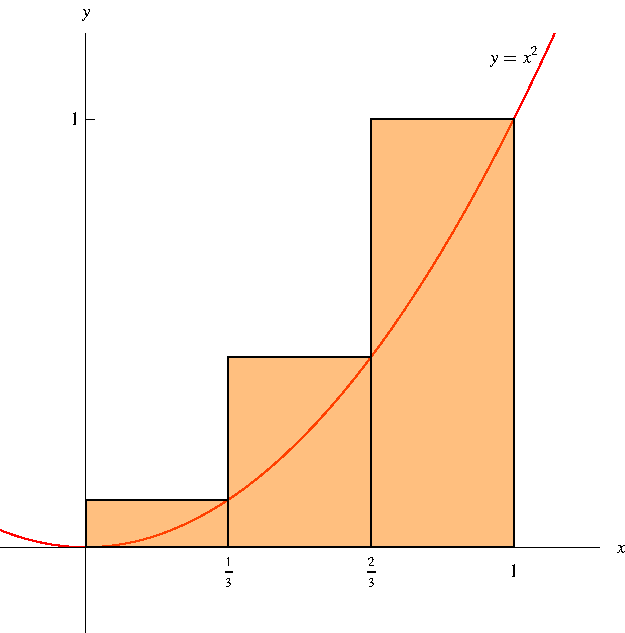
\includegraphics[height=4.2cm]{integration/pictures/05-01-righta.pdf}%
%}%
%\only<handout:0| 2>{%
%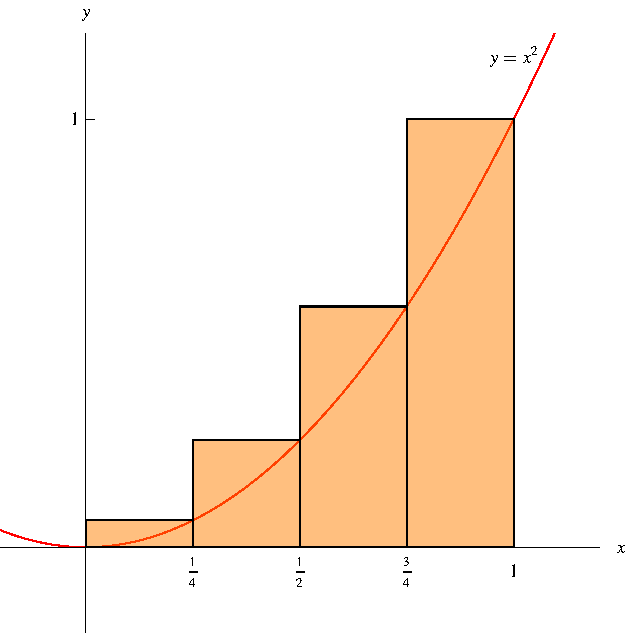
\includegraphics[height=4.2cm]{integration/pictures/05-01-rightb.pdf}%
%}%
%\only<handout:0| 3>{%
%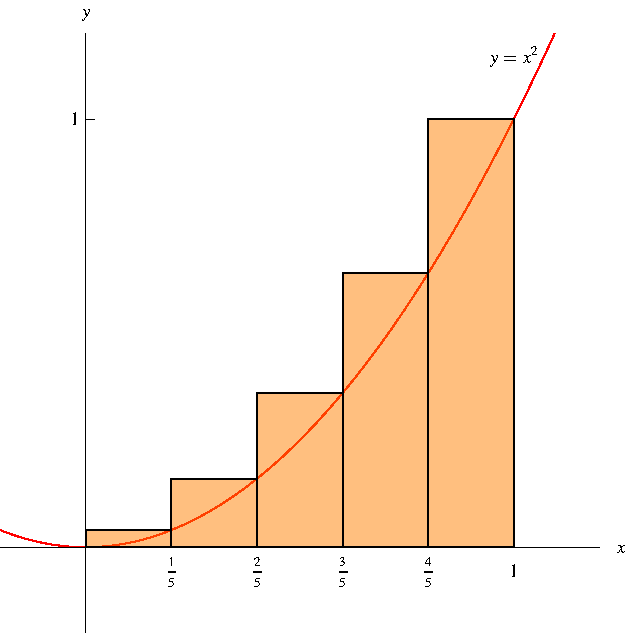
\includegraphics[height=4.2cm]{integration/pictures/05-01-rightc.pdf}%
%}%
%\only<handout:0| 4>{%
%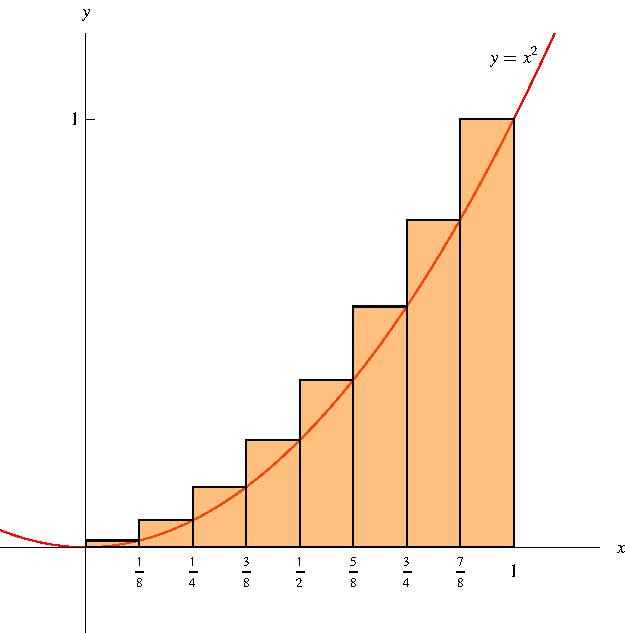
\includegraphics[height=4.2cm]{integration/pictures/05-01-rightd.pdf}%
%}%
%\only<handout:0| 5>{%
%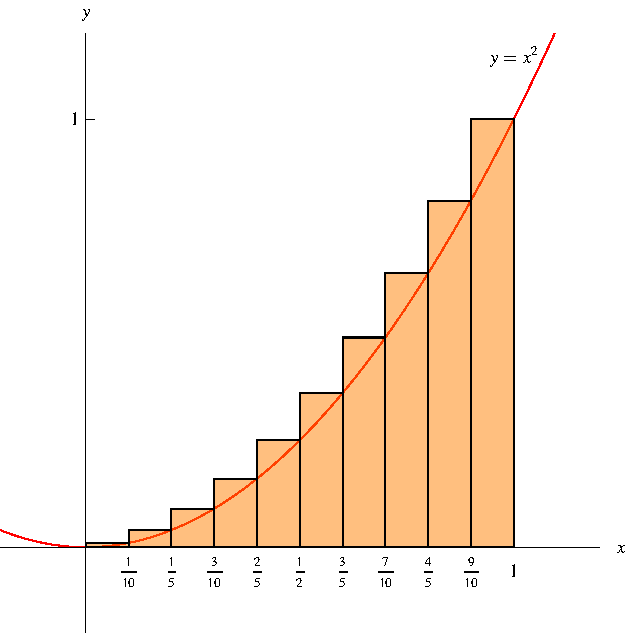
\includegraphics[height=4.2cm]{integration/pictures/05-01-righte.pdf}%
%}%
%\only<handout:0| 6>{%
%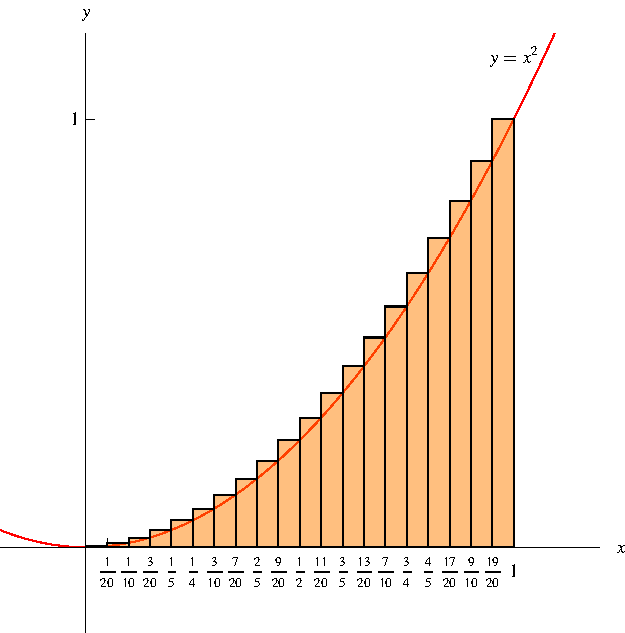
\includegraphics[height=4.2cm]{integration/pictures/05-01-rightf.pdf}%
%}%
%\only<handout:0| 7>{%
%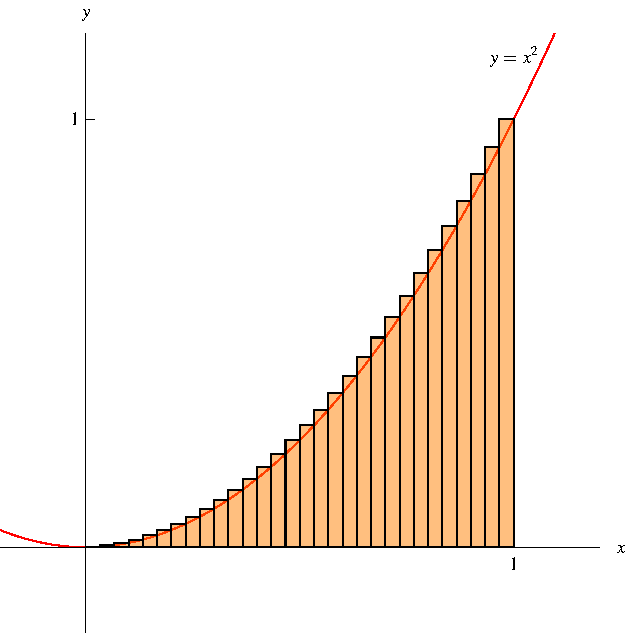
\includegraphics[height=4.2cm]{integration/pictures/05-01-rightg.pdf}%
%}%
%\only<handout:0| 8>{%
%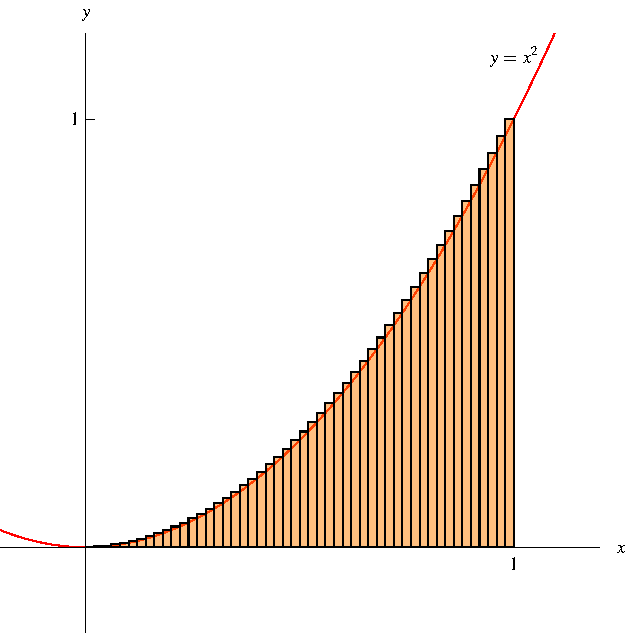
\includegraphics[height=4.2cm]{integration/pictures/05-01-righth.pdf}%
%}%
%\only<handout:1| 9->{%
%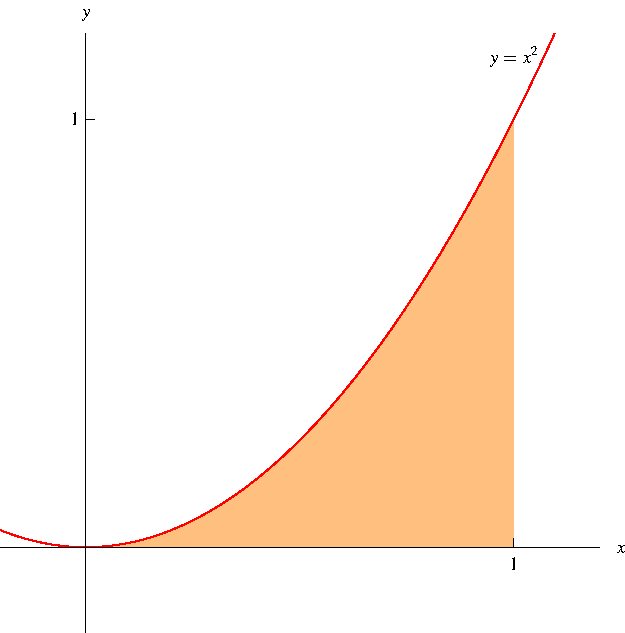
\includegraphics[height=4.2cm]{integration/pictures/05-01-xsquaredarea.pdf}%
%}%
\end{columns}
\begin{columns}
\column{.4\textwidth}


\uncover<10->{%
\psset{xunit=2cm, yunit=2cm}
\begin{pspicture}(-0.15,-1.6)(1.5,1.4)
\psframe*[linecolor=white](-0.15,-1.6)(1.5,1.4)
\tiny
\rput (1, 0.8){$y=f(x)$}
\uncover<handout:0|11>{
\psline*[linecolor=\fcColorNegativeAreaUnderGraph, linewidth=0.1pt](0.45, 0)(0.45, -0.582187)(0.1, -0.582187)(0.1, 0)
\psline*[linecolor=\fcColorAreaUnderGraph, linewidth=0.1pt](0.8, 0)(0.8, 0.512)(0.45, 0.512)(0.45, 0)(1.15, 0)(1.15, 0.142313)(0.8, 0.142313)(0.8, 0)
\psline*[linecolor=\fcColorNegativeAreaUnderGraph, linewidth=0.1pt](1.5, 0)(1.5, -0.405)(1.15, -0.405)(1.15, 0)
\psline[linecolor=brown, linewidth=0.1pt](0.45, 0)(0.45, -0.582187)(0.1, -0.582187)(0.1, 0)
\psline[linecolor=blue, linewidth=0.1pt](0.8, 0)(0.8, 0.512)(0.45, 0.512)(0.45, 0)(1.15, 0)(1.15, 0.142313)(0.8, 0.142313)(0.8, 0)
\psline[linecolor=brown, linewidth=0.1pt](1.5, 0)(1.5, -0.405)(1.15, -0.405)(1.15, 0)
}
\uncover<handout:0|12>{
\psline*[linecolor=\fcColorNegativeAreaUnderGraph, linewidth=0.1pt](0.333333, 0)(0.333333, -0.975802)(0.1, -0.975802)(0.1, 0)(0.566667, 0)(0.566667, -0.123617)(0.333333, -0.123617)(0.333333, 0)
\psline*[linecolor=\fcColorAreaUnderGraph, linewidth=0.1pt](0.8, 0)(0.8, 0.512)(0.566667, 0.512)(0.566667, 0)(1.03333, 0)(1.03333, 0.422901)(0.8, 0.422901)(0.8, 0)
\psline*[linecolor=\fcColorNegativeAreaUnderGraph, linewidth=0.1pt](1.26667, 0)(1.26667, -0.187654)(1.03333, -0.187654)(1.03333, 0)(1.5, 0)(1.5, -0.405)(1.26667, -0.405)(1.26667, 0)
\psline[linecolor=brown, linewidth=0.1pt](0.333333, 0)(0.333333, -0.975802)(0.1, -0.975802)(0.1, 0)(0.566667, 0)(0.566667, -0.123617)(0.333333, -0.123617)(0.333333, 0)
\psline[linecolor=blue, linewidth=0.1pt](0.8, 0)(0.8, 0.512)(0.566667, 0.512)(0.566667, 0)(1.03333, 0)(1.03333, 0.422901)(0.8, 0.422901)(0.8, 0)
\psline[linecolor=brown, linewidth=0.1pt](1.26667, 0)(1.26667, -0.187654)(1.03333, -0.187654)(1.03333, 0)(1.5, 0)(1.5, -0.405)(1.26667, -0.405)(1.26667, 0)
}
\uncover<handout:0|13>{
\psline*[linecolor=\fcColorNegativeAreaUnderGraph, linewidth=0.1pt](0.275, 0)(0.275, -1.0954)(0.1, -1.0954)(0.1, 0)(0.45, 0)(0.45, -0.582187)(0.275, -0.582187)(0.275, 0)
\psline*[linecolor=\fcColorAreaUnderGraph, linewidth=0.1pt](0.625, 0)(0.625, 0.0875977)(0.45, 0.0875977)(0.45, 0)(0.8, 0)(0.8, 0.512)(0.625, 0.512)(0.625, 0)(0.975, 0)(0.975, 0.51416)(0.8, 0.51416)(0.8, 0)(1.15, 0)(1.15, 0.142313)(0.975, 0.142313)(0.975, 0)
\psline*[linecolor=\fcColorNegativeAreaUnderGraph, linewidth=0.1pt](1.325, 0)(1.325, -0.330215)(1.15, -0.330215)(1.15, 0)(1.5, 0)(1.5, -0.405)(1.325, -0.405)(1.325, 0)
\psline[linecolor=brown, linewidth=0.1pt](0.275, 0)(0.275, -1.0954)(0.1, -1.0954)(0.1, 0)(0.45, 0)(0.45, -0.582187)(0.275, -0.582187)(0.275, 0)
\psline[linecolor=blue, linewidth=0.1pt](0.625, 0)(0.625, 0.0875977)(0.45, 0.0875977)(0.45, 0)(0.8, 0)(0.8, 0.512)(0.625, 0.512)(0.625, 0)(0.975, 0)(0.975, 0.51416)(0.8, 0.51416)(0.8, 0)(1.15, 0)(1.15, 0.142313)(0.975, 0.142313)(0.975, 0)
\psline[linecolor=brown, linewidth=0.1pt](1.325, 0)(1.325, -0.330215)(1.15, -0.330215)(1.15, 0)(1.5, 0)(1.5, -0.405)(1.325, -0.405)(1.325, 0)
}
\uncover<handout:0|14>{
\psline*[linecolor=\fcColorNegativeAreaUnderGraph, linewidth=0.1pt](0.24, 0)(0.24, -1.12804)(0.1, -1.12804)(0.1, 0)(0.38, 0)(0.38, -0.836334)(0.24, -0.836334)(0.24, 0)(0.52, 0)(0.52, -0.30551)(0.38, -0.30551)(0.38, 0)
\psline*[linecolor=\fcColorAreaUnderGraph, linewidth=0.1pt](0.66, 0)(0.66, 0.20101)(0.52, 0.20101)(0.52, 0)(0.8, 0)(0.8, 0.512)(0.66, 0.512)(0.66, 0)(0.94, 0)(0.94, 0.548434)(0.8, 0.548434)(0.8, 0)(1.08, 0)(1.08, 0.323482)(0.94, 0.323482)(0.94, 0)
\psline*[linecolor=\fcColorNegativeAreaUnderGraph, linewidth=0.1pt](1.22, 0)(1.22, -0.0574864)(1.08, -0.0574864)(1.08, 0)(1.36, 0)(1.36, -0.396902)(1.22, -0.396902)(1.22, 0)(1.5, 0)(1.5, -0.405)(1.36, -0.405)(1.36, 0)
\psline[linecolor=brown, linewidth=0.1pt](0.24, 0)(0.24, -1.12804)(0.1, -1.12804)(0.1, 0)(0.38, 0)(0.38, -0.836334)(0.24, -0.836334)(0.24, 0)(0.52, 0)(0.52, -0.30551)(0.38, -0.30551)(0.38, 0)
\psline[linecolor=blue, linewidth=0.1pt](0.66, 0)(0.66, 0.20101)(0.52, 0.20101)(0.52, 0)(0.8, 0)(0.8, 0.512)(0.66, 0.512)(0.66, 0)(0.94, 0)(0.94, 0.548434)(0.8, 0.548434)(0.8, 0)(1.08, 0)(1.08, 0.323482)(0.94, 0.323482)(0.94, 0)
\psline[linecolor=brown, linewidth=0.1pt](1.22, 0)(1.22, -0.0574864)(1.08, -0.0574864)(1.08, 0)(1.36, 0)(1.36, -0.396902)(1.22, -0.396902)(1.22, 0)(1.5, 0)(1.5, -0.405)(1.36, -0.405)(1.36, 0)
}
\uncover<handout:1|15>{
\psline*[linecolor=\fcColorNegativeAreaUnderGraph, linewidth=0.1pt](0.193333, 0)(0.193333, -1.11333)(0.1, -1.11333)(0.1, 0)(0.286667, 0)(0.286667, -1.07743)(0.193333, -1.07743)(0.193333, 0)(0.38, 0)(0.38, -0.836334)(0.286667, -0.836334)(0.286667, 0)(0.473333, 0)(0.473333, -0.490863)(0.38, -0.490863)(0.38, 0)(0.566667, 0)(0.566667, -0.123617)(0.473333, -0.123617)(0.473333, 0)
\psline*[linecolor=\fcColorAreaUnderGraph, linewidth=0.1pt](0.66, 0)(0.66, 0.20101)(0.566667, 0.20101)(0.566667, 0)(0.753333, 0)(0.753333, 0.436837)(0.66, 0.436837)(0.66, 0)(0.846667, 0)(0.846667, 0.555898)(0.753333, 0.555898)(0.753333, 0)(0.94, 0)(0.94, 0.548434)(0.846667, 0.548434)(0.846667, 0)(1.03333, 0)(1.03333, 0.422901)(0.94, 0.422901)(0.94, 0)(1.12667, 0)(1.12667, 0.205968)(1.03333, 0.205968)(1.03333, 0)
\psline*[linecolor=\fcColorNegativeAreaUnderGraph, linewidth=0.1pt](1.22, 0)(1.22, -0.0574864)(1.12667, -0.0574864)(1.12667, 0)(1.31333, 0)(1.31333, -0.30437)(1.22, -0.30437)(1.22, 0)(1.40667, 0)(1.40667, -0.45338)(1.31333, -0.45338)(1.31333, 0)(1.5, 0)(1.5, -0.405)(1.40667, -0.405)(1.40667, 0)
\psline[linecolor=brown, linewidth=0.1pt](0.193333, 0)(0.193333, -1.11333)(0.1, -1.11333)(0.1, 0)(0.286667, 0)(0.286667, -1.07743)(0.193333, -1.07743)(0.193333, 0)(0.38, 0)(0.38, -0.836334)(0.286667, -0.836334)(0.286667, 0)(0.473333, 0)(0.473333, -0.490863)(0.38, -0.490863)(0.38, 0)(0.566667, 0)(0.566667, -0.123617)(0.473333, -0.123617)(0.473333, 0)
\psline[linecolor=blue, linewidth=0.1pt](0.66, 0)(0.66, 0.20101)(0.566667, 0.20101)(0.566667, 0)(0.753333, 0)(0.753333, 0.436837)(0.66, 0.436837)(0.66, 0)(0.846667, 0)(0.846667, 0.555898)(0.753333, 0.555898)(0.753333, 0)(0.94, 0)(0.94, 0.548434)(0.846667, 0.548434)(0.846667, 0)(1.03333, 0)(1.03333, 0.422901)(0.94, 0.422901)(0.94, 0)(1.12667, 0)(1.12667, 0.205968)(1.03333, 0.205968)(1.03333, 0)
\psline[linecolor=brown, linewidth=0.1pt](1.22, 0)(1.22, -0.0574864)(1.12667, -0.0574864)(1.12667, 0)(1.31333, 0)(1.31333, -0.30437)(1.22, -0.30437)(1.22, 0)(1.40667, 0)(1.40667, -0.45338)(1.31333, -0.45338)(1.31333, 0)(1.5, 0)(1.5, -0.405)(1.40667, -0.405)(1.40667, 0)
}
\uncover<handout:0|16>{
\psline*[linecolor=\fcColorNegativeAreaUnderGraph, linewidth=0.1pt](0.17, 0)(0.17, -1.07669)(0.1, -1.07669)(0.1, 0)(0.24, 0)(0.24, -1.12804)(0.17, -1.12804)(0.17, 0)(0.31, 0)(0.31, -1.03214)(0.24, -1.03214)(0.24, 0)(0.38, 0)(0.38, -0.836334)(0.31, -0.836334)(0.31, 0)(0.45, 0)(0.45, -0.582187)(0.38, -0.582187)(0.38, 0)(0.52, 0)(0.52, -0.30551)(0.45, -0.30551)(0.45, 0)(0.59, 0)(0.59, -0.0363499)(0.52, -0.0363499)(0.52, 0)
\psline*[linecolor=\fcColorAreaUnderGraph, linewidth=0.1pt](0.66, 0)(0.66, 0.20101)(0.59, 0.20101)(0.59, 0)(0.73, 0)(0.73, 0.388046)(0.66, 0.388046)(0.66, 0)(0.8, 0)(0.8, 0.512)(0.73, 0.512)(0.73, 0)(0.87, 0)(0.87, 0.565874)(0.8, 0.565874)(0.8, 0)(0.94, 0)(0.94, 0.548434)(0.87, 0.548434)(0.87, 0)(1.01, 0)(1.01, 0.464206)(0.94, 0.464206)(0.94, 0)(1.08, 0)(1.08, 0.323482)(1.01, 0.323482)(1.01, 0)(1.15, 0)(1.15, 0.142313)(1.08, 0.142313)(1.08, 0)
\psline*[linecolor=\fcColorNegativeAreaUnderGraph, linewidth=0.1pt](1.22, 0)(1.22, -0.0574864)(1.15, -0.0574864)(1.15, 0)(1.29, 0)(1.29, -0.248338)(1.22, -0.248338)(1.22, 0)(1.36, 0)(1.36, -0.396902)(1.29, -0.396902)(1.29, 0)(1.43, 0)(1.43, -0.464078)(1.36, -0.464078)(1.36, 0)(1.5, 0)(1.5, -0.405)(1.43, -0.405)(1.43, 0)
\psline[linecolor=brown, linewidth=0.1pt](0.17, 0)(0.17, -1.07669)(0.1, -1.07669)(0.1, 0)(0.24, 0)(0.24, -1.12804)(0.17, -1.12804)(0.17, 0)(0.31, 0)(0.31, -1.03214)(0.24, -1.03214)(0.24, 0)(0.38, 0)(0.38, -0.836334)(0.31, -0.836334)(0.31, 0)(0.45, 0)(0.45, -0.582187)(0.38, -0.582187)(0.38, 0)(0.52, 0)(0.52, -0.30551)(0.45, -0.30551)(0.45, 0)(0.59, 0)(0.59, -0.0363499)(0.52, -0.0363499)(0.52, 0)
\psline[linecolor=blue, linewidth=0.1pt](0.66, 0)(0.66, 0.20101)(0.59, 0.20101)(0.59, 0)(0.73, 0)(0.73, 0.388046)(0.66, 0.388046)(0.66, 0)(0.8, 0)(0.8, 0.512)(0.73, 0.512)(0.73, 0)(0.87, 0)(0.87, 0.565874)(0.8, 0.565874)(0.8, 0)(0.94, 0)(0.94, 0.548434)(0.87, 0.548434)(0.87, 0)(1.01, 0)(1.01, 0.464206)(0.94, 0.464206)(0.94, 0)(1.08, 0)(1.08, 0.323482)(1.01, 0.323482)(1.01, 0)(1.15, 0)(1.15, 0.142313)(1.08, 0.142313)(1.08, 0)
\psline[linecolor=brown, linewidth=0.1pt](1.22, 0)(1.22, -0.0574864)(1.15, -0.0574864)(1.15, 0)(1.29, 0)(1.29, -0.248338)(1.22, -0.248338)(1.22, 0)(1.36, 0)(1.36, -0.396902)(1.29, -0.396902)(1.29, 0)(1.43, 0)(1.43, -0.464078)(1.36, -0.464078)(1.36, 0)(1.5, 0)(1.5, -0.405)(1.43, -0.405)(1.43, 0)
}
\uncover<handout:0|17>{
\psline*[linecolor=\fcColorNegativeAreaUnderGraph, linewidth=0.1pt](0.146667, 0)(0.146667, -1.01784)(0.1, -1.01784)(0.1, 0)(0.193333, 0)(0.193333, -1.11333)(0.146667, -1.11333)(0.146667, 0)(0.24, 0)(0.24, -1.12804)(0.193333, -1.12804)(0.193333, 0)(0.286667, 0)(0.286667, -1.07743)(0.24, -1.07743)(0.24, 0)(0.333333, 0)(0.333333, -0.975802)(0.286667, -0.975802)(0.286667, 0)(0.38, 0)(0.38, -0.836334)(0.333333, -0.836334)(0.333333, 0)(0.426667, 0)(0.426667, -0.671056)(0.38, -0.671056)(0.38, 0)(0.473333, 0)(0.473333, -0.490863)(0.426667, -0.490863)(0.426667, 0)(0.52, 0)(0.52, -0.30551)(0.473333, -0.30551)(0.473333, 0)(0.566667, 0)(0.566667, -0.123617)(0.52, -0.123617)(0.52, 0)
\psline*[linecolor=\fcColorAreaUnderGraph, linewidth=0.1pt](0.613333, 0)(0.613333, 0.0473366)(0.566667, 0.0473366)(0.566667, 0)(0.66, 0)(0.66, 0.20101)(0.613333, 0.20101)(0.613333, 0)(0.706667, 0)(0.706667, 0.332198)(0.66, 0.332198)(0.66, 0)(0.753333, 0)(0.753333, 0.436837)(0.706667, 0.436837)(0.706667, 0)(0.8, 0)(0.8, 0.512)(0.753333, 0.512)(0.753333, 0)(0.846667, 0)(0.846667, 0.555898)(0.8, 0.555898)(0.8, 0)(0.893333, 0)(0.893333, 0.567879)(0.846667, 0.567879)(0.846667, 0)(0.94, 0)(0.94, 0.548434)(0.893333, 0.548434)(0.893333, 0)(0.986667, 0)(0.986667, 0.499186)(0.94, 0.499186)(0.94, 0)(1.03333, 0)(1.03333, 0.422901)(0.986667, 0.422901)(0.986667, 0)(1.08, 0)(1.08, 0.323482)(1.03333, 0.323482)(1.03333, 0)(1.12667, 0)(1.12667, 0.205968)(1.08, 0.205968)(1.08, 0)(1.17333, 0)(1.17333, 0.0765396)(1.12667, 0.0765396)(1.12667, 0)
\psline*[linecolor=\fcColorNegativeAreaUnderGraph, linewidth=0.1pt](1.22, 0)(1.22, -0.0574864)(1.17333, -0.0574864)(1.17333, 0)(1.26667, 0)(1.26667, -0.187654)(1.22, -0.187654)(1.22, 0)(1.31333, 0)(1.31333, -0.30437)(1.26667, -0.30437)(1.26667, 0)(1.36, 0)(1.36, -0.396902)(1.31333, -0.396902)(1.31333, 0)(1.40667, 0)(1.40667, -0.45338)(1.36, -0.45338)(1.36, 0)(1.45333, 0)(1.45333, -0.460795)(1.40667, -0.460795)(1.40667, 0)(1.5, 0)(1.5, -0.405)(1.45333, -0.405)(1.45333, 0)
\psline[linecolor=brown, linewidth=0.1pt](0.146667, 0)(0.146667, -1.01784)(0.1, -1.01784)(0.1, 0)(0.193333, 0)(0.193333, -1.11333)(0.146667, -1.11333)(0.146667, 0)(0.24, 0)(0.24, -1.12804)(0.193333, -1.12804)(0.193333, 0)(0.286667, 0)(0.286667, -1.07743)(0.24, -1.07743)(0.24, 0)(0.333333, 0)(0.333333, -0.975802)(0.286667, -0.975802)(0.286667, 0)(0.38, 0)(0.38, -0.836334)(0.333333, -0.836334)(0.333333, 0)(0.426667, 0)(0.426667, -0.671056)(0.38, -0.671056)(0.38, 0)(0.473333, 0)(0.473333, -0.490863)(0.426667, -0.490863)(0.426667, 0)(0.52, 0)(0.52, -0.30551)(0.473333, -0.30551)(0.473333, 0)(0.566667, 0)(0.566667, -0.123617)(0.52, -0.123617)(0.52, 0)
\psline[linecolor=blue, linewidth=0.1pt](0.613333, 0)(0.613333, 0.0473366)(0.566667, 0.0473366)(0.566667, 0)(0.66, 0)(0.66, 0.20101)(0.613333, 0.20101)(0.613333, 0)(0.706667, 0)(0.706667, 0.332198)(0.66, 0.332198)(0.66, 0)(0.753333, 0)(0.753333, 0.436837)(0.706667, 0.436837)(0.706667, 0)(0.8, 0)(0.8, 0.512)(0.753333, 0.512)(0.753333, 0)(0.846667, 0)(0.846667, 0.555898)(0.8, 0.555898)(0.8, 0)(0.893333, 0)(0.893333, 0.567879)(0.846667, 0.567879)(0.846667, 0)(0.94, 0)(0.94, 0.548434)(0.893333, 0.548434)(0.893333, 0)(0.986667, 0)(0.986667, 0.499186)(0.94, 0.499186)(0.94, 0)(1.03333, 0)(1.03333, 0.422901)(0.986667, 0.422901)(0.986667, 0)(1.08, 0)(1.08, 0.323482)(1.03333, 0.323482)(1.03333, 0)(1.12667, 0)(1.12667, 0.205968)(1.08, 0.205968)(1.08, 0)(1.17333, 0)(1.17333, 0.0765396)(1.12667, 0.0765396)(1.12667, 0)
\psline[linecolor=brown, linewidth=0.1pt](1.22, 0)(1.22, -0.0574864)(1.17333, -0.0574864)(1.17333, 0)(1.26667, 0)(1.26667, -0.187654)(1.22, -0.187654)(1.22, 0)(1.31333, 0)(1.31333, -0.30437)(1.26667, -0.30437)(1.26667, 0)(1.36, 0)(1.36, -0.396902)(1.31333, -0.396902)(1.31333, 0)(1.40667, 0)(1.40667, -0.45338)(1.36, -0.45338)(1.36, 0)(1.45333, 0)(1.45333, -0.460795)(1.40667, -0.460795)(1.40667, 0)(1.5, 0)(1.5, -0.405)(1.45333, -0.405)(1.45333, 0)
}
\uncover<handout:0|18>{
\psline*[linecolor=\fcColorNegativeAreaUnderGraph, linewidth=0.1pt](0.135, 0)(0.135, -0.979431)(0.1, -0.979431)(0.1, 0)(0.17, 0)(0.17, -1.07669)(0.135, -1.07669)(0.135, 0)(0.205, 0)(0.205, -1.12395)(0.17, -1.12395)(0.17, 0)(0.24, 0)(0.24, -1.12804)(0.205, -1.12804)(0.205, 0)(0.275, 0)(0.275, -1.0954)(0.24, -1.0954)(0.24, 0)(0.31, 0)(0.31, -1.03214)(0.275, -1.03214)(0.275, 0)(0.345, 0)(0.345, -0.943994)(0.31, -0.943994)(0.31, 0)(0.38, 0)(0.38, -0.836334)(0.345, -0.836334)(0.345, 0)(0.415, 0)(0.415, -0.71418)(0.38, -0.71418)(0.38, 0)(0.45, 0)(0.45, -0.582187)(0.415, -0.582187)(0.415, 0)(0.485, 0)(0.485, -0.444652)(0.45, -0.444652)(0.45, 0)(0.52, 0)(0.52, -0.30551)(0.485, -0.30551)(0.485, 0)(0.555, 0)(0.555, -0.168338)(0.52, -0.168338)(0.52, 0)(0.59, 0)(0.59, -0.0363499)(0.555, -0.0363499)(0.555, 0)
\psline*[linecolor=\fcColorAreaUnderGraph, linewidth=0.1pt](0.625, 0)(0.625, 0.0875977)(0.59, 0.0875977)(0.59, 0)(0.66, 0)(0.66, 0.20101)(0.625, 0.20101)(0.625, 0)(0.695, 0)(0.695, 0.301751)(0.66, 0.301751)(0.66, 0)(0.73, 0)(0.73, 0.388046)(0.695, 0.388046)(0.695, 0)(0.765, 0)(0.765, 0.458481)(0.73, 0.458481)(0.73, 0)(0.8, 0)(0.8, 0.512)(0.765, 0.512)(0.765, 0)(0.835, 0)(0.835, 0.547909)(0.8, 0.547909)(0.8, 0)(0.87, 0)(0.87, 0.565874)(0.835, 0.565874)(0.835, 0)(0.905, 0)(0.905, 0.56592)(0.87, 0.56592)(0.87, 0)(0.94, 0)(0.94, 0.548434)(0.905, 0.548434)(0.905, 0)(0.975, 0)(0.975, 0.51416)(0.94, 0.51416)(0.94, 0)(1.01, 0)(1.01, 0.464206)(0.975, 0.464206)(0.975, 0)(1.045, 0)(1.045, 0.400038)(1.01, 0.400038)(1.01, 0)(1.08, 0)(1.08, 0.323482)(1.045, 0.323482)(1.045, 0)(1.115, 0)(1.115, 0.236724)(1.08, 0.236724)(1.08, 0)(1.15, 0)(1.15, 0.142313)(1.115, 0.142313)(1.115, 0)(1.185, 0)(1.185, 0.0431533)(1.15, 0.0431533)(1.15, 0)
\psline*[linecolor=\fcColorNegativeAreaUnderGraph, linewidth=0.1pt](1.22, 0)(1.22, -0.0574864)(1.185, -0.0574864)(1.185, 0)(1.255, 0)(1.255, -0.155979)(1.22, -0.155979)(1.22, 0)(1.29, 0)(1.29, -0.248338)(1.255, -0.248338)(1.255, 0)(1.325, 0)(1.325, -0.330215)(1.29, -0.330215)(1.29, 0)(1.36, 0)(1.36, -0.396902)(1.325, -0.396902)(1.325, 0)(1.395, 0)(1.395, -0.443333)(1.36, -0.443333)(1.36, 0)(1.43, 0)(1.43, -0.464078)(1.395, -0.464078)(1.395, 0)(1.465, 0)(1.465, -0.45335)(1.43, -0.45335)(1.43, 0)(1.5, 0)(1.5, -0.405)(1.465, -0.405)(1.465, 0)
\psline[linecolor=brown, linewidth=0.1pt](0.135, 0)(0.135, -0.979431)(0.1, -0.979431)(0.1, 0)(0.17, 0)(0.17, -1.07669)(0.135, -1.07669)(0.135, 0)(0.205, 0)(0.205, -1.12395)(0.17, -1.12395)(0.17, 0)(0.24, 0)(0.24, -1.12804)(0.205, -1.12804)(0.205, 0)(0.275, 0)(0.275, -1.0954)(0.24, -1.0954)(0.24, 0)(0.31, 0)(0.31, -1.03214)(0.275, -1.03214)(0.275, 0)(0.345, 0)(0.345, -0.943994)(0.31, -0.943994)(0.31, 0)(0.38, 0)(0.38, -0.836334)(0.345, -0.836334)(0.345, 0)(0.415, 0)(0.415, -0.71418)(0.38, -0.71418)(0.38, 0)(0.45, 0)(0.45, -0.582187)(0.415, -0.582187)(0.415, 0)(0.485, 0)(0.485, -0.444652)(0.45, -0.444652)(0.45, 0)(0.52, 0)(0.52, -0.30551)(0.485, -0.30551)(0.485, 0)(0.555, 0)(0.555, -0.168338)(0.52, -0.168338)(0.52, 0)(0.59, 0)(0.59, -0.0363499)(0.555, -0.0363499)(0.555, 0)
\psline[linecolor=blue, linewidth=0.1pt](0.625, 0)(0.625, 0.0875977)(0.59, 0.0875977)(0.59, 0)(0.66, 0)(0.66, 0.20101)(0.625, 0.20101)(0.625, 0)(0.695, 0)(0.695, 0.301751)(0.66, 0.301751)(0.66, 0)(0.73, 0)(0.73, 0.388046)(0.695, 0.388046)(0.695, 0)(0.765, 0)(0.765, 0.458481)(0.73, 0.458481)(0.73, 0)(0.8, 0)(0.8, 0.512)(0.765, 0.512)(0.765, 0)(0.835, 0)(0.835, 0.547909)(0.8, 0.547909)(0.8, 0)(0.87, 0)(0.87, 0.565874)(0.835, 0.565874)(0.835, 0)(0.905, 0)(0.905, 0.56592)(0.87, 0.56592)(0.87, 0)(0.94, 0)(0.94, 0.548434)(0.905, 0.548434)(0.905, 0)(0.975, 0)(0.975, 0.51416)(0.94, 0.51416)(0.94, 0)(1.01, 0)(1.01, 0.464206)(0.975, 0.464206)(0.975, 0)(1.045, 0)(1.045, 0.400038)(1.01, 0.400038)(1.01, 0)(1.08, 0)(1.08, 0.323482)(1.045, 0.323482)(1.045, 0)(1.115, 0)(1.115, 0.236724)(1.08, 0.236724)(1.08, 0)(1.15, 0)(1.15, 0.142313)(1.115, 0.142313)(1.115, 0)(1.185, 0)(1.185, 0.0431533)(1.15, 0.0431533)(1.15, 0)
\psline[linecolor=brown, linewidth=0.1pt](1.22, 0)(1.22, -0.0574864)(1.185, -0.0574864)(1.185, 0)(1.255, 0)(1.255, -0.155979)(1.22, -0.155979)(1.22, 0)(1.29, 0)(1.29, -0.248338)(1.255, -0.248338)(1.255, 0)(1.325, 0)(1.325, -0.330215)(1.29, -0.330215)(1.29, 0)(1.36, 0)(1.36, -0.396902)(1.325, -0.396902)(1.325, 0)(1.395, 0)(1.395, -0.443333)(1.36, -0.443333)(1.36, 0)(1.43, 0)(1.43, -0.464078)(1.395, -0.464078)(1.395, 0)(1.465, 0)(1.465, -0.45335)(1.43, -0.45335)(1.43, 0)(1.5, 0)(1.5, -0.405)(1.465, -0.405)(1.465, 0)
}

\uncover<handout:2|19->{
\pscustom*[linecolor=\fcColorNegativeAreaUnderGraph]{
\psplot{0.1}{0.6}{x 3 exp -34 mul x -11.52 mul x 4 exp 10 mul x 2 exp 36 mul add add add }
\psline(0.6,0)(0.1,0)
}
\pscustom*[linecolor=\fcColorAreaUnderGraph]{
\psplot{0.6}{1.2}{x 3 exp -34 mul x -11.52 mul x 4 exp 10 mul x 2 exp 36 mul add add add }
\psline(1.2,0)(0.6,0)
}
\pscustom*[linecolor=\fcColorNegativeAreaUnderGraph]{
\psplot{1.2}{1.5}{x 3 exp -34 mul x -11.52 mul x 4 exp 10 mul x 2 exp 36 mul add add add }
\psline(1.5,0)(1.2,0)
}
}
\psaxes[ticks=none, labels=none]{<->}(0,0)(-0.1,-1.2)(2,1)
\psplot[linecolor=red, plotpoints=1000]{0.1}{1.5}{x 3 exp -34 mul x -11.52 mul x 4 exp 10 mul x 2 exp 36 mul add add add }
\uncover<handout:2|19->{
\rput (0.9, 0.3){$A_1$}
\rput[t](0.9, -0.5){$A_2$}
\psline{->}(0.85, -0.45)(0.35, -0.3)
\psline{->}(0.95, -0.45)(1.4, -0.2)
}
\end{pspicture}
%\only<handout:0| -10>{%
%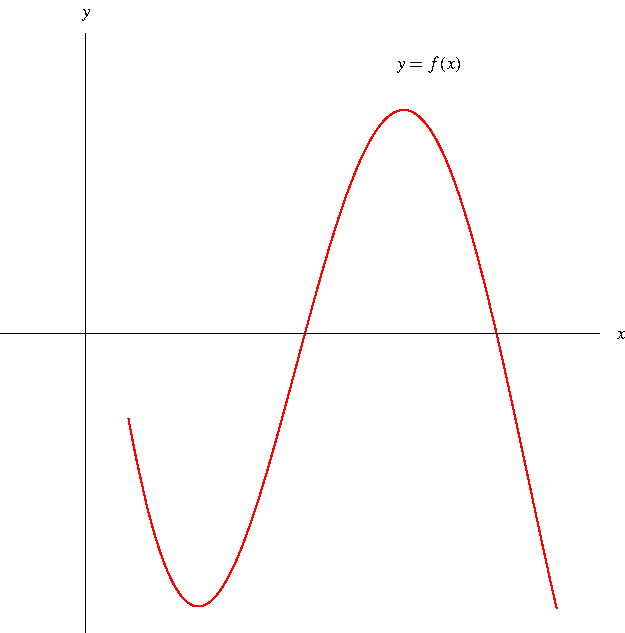
\includegraphics[height=4.2cm]{integration/pictures/05-02-net-area-function.pdf}%
%}%
%\only<handout:0| 11>{%
%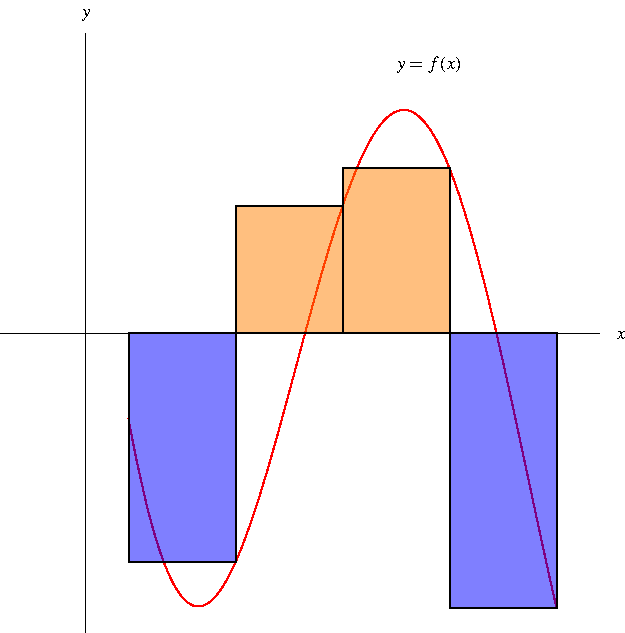
\includegraphics[height=4.2cm]{integration/pictures/05-02-net-areaa.pdf}%
%}%
%\only<handout:0| 12>{%
%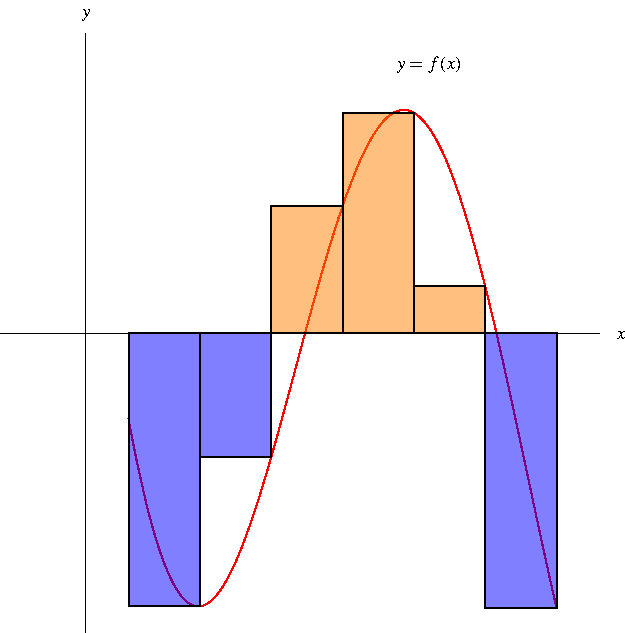
\includegraphics[height=4.2cm]{integration/pictures/05-02-net-areab.pdf}%
%}%
%\only<handout:0| 13>{%
%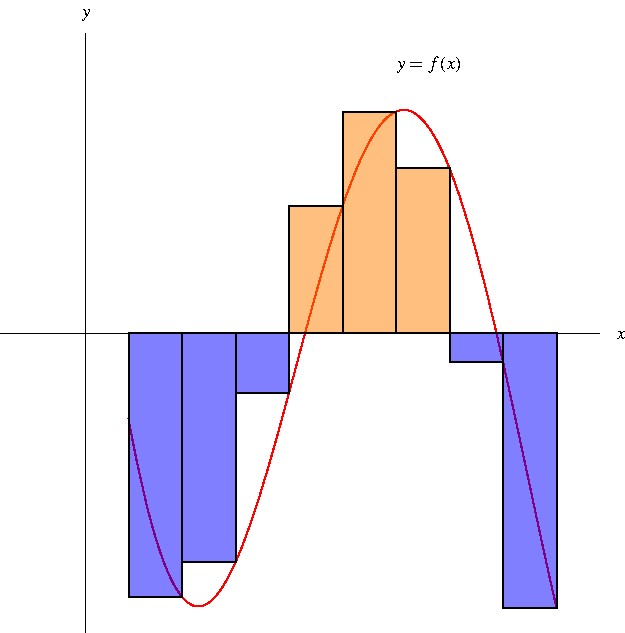
\includegraphics[height=4.2cm]{integration/pictures/05-02-net-areac.pdf}%
%}%
%\only<handout:0| 14>{%
%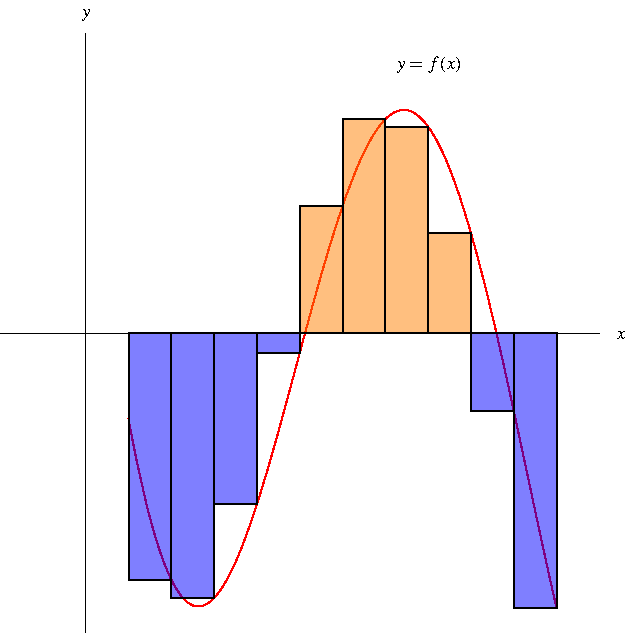
\includegraphics[height=4.2cm]{integration/pictures/05-02-net-aread.pdf}%
%}%
%\only<handout:0| 15>{%
%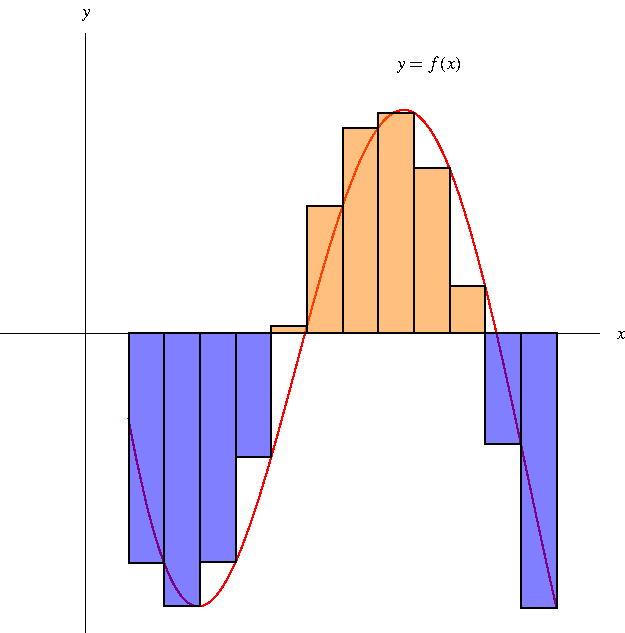
\includegraphics[height=4.2cm]{integration/pictures/05-02-net-areae.pdf}%
%}%
%\only<handout:0| 16>{%
%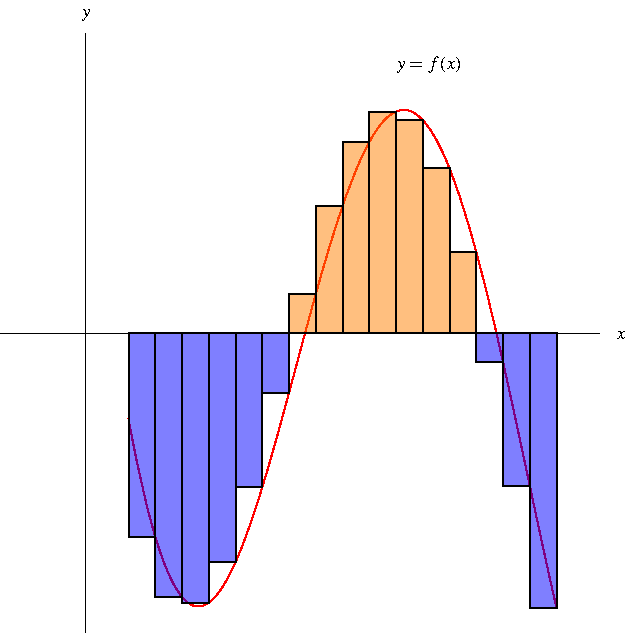
\includegraphics[height=4.2cm]{integration/pictures/05-02-net-areaf.pdf}%
%}%
%\only<handout:0| 17>{%
%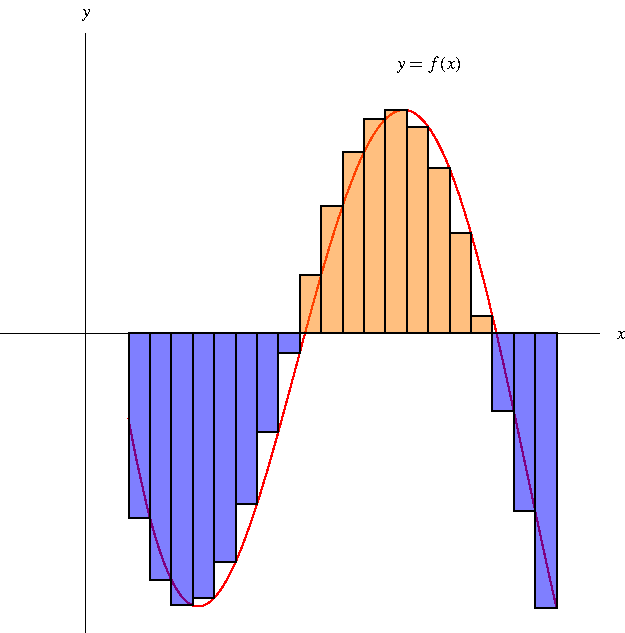
\includegraphics[height=4.2cm]{integration/pictures/05-02-net-areag.pdf}%
%}%
%\only<handout:0| 18>{%
%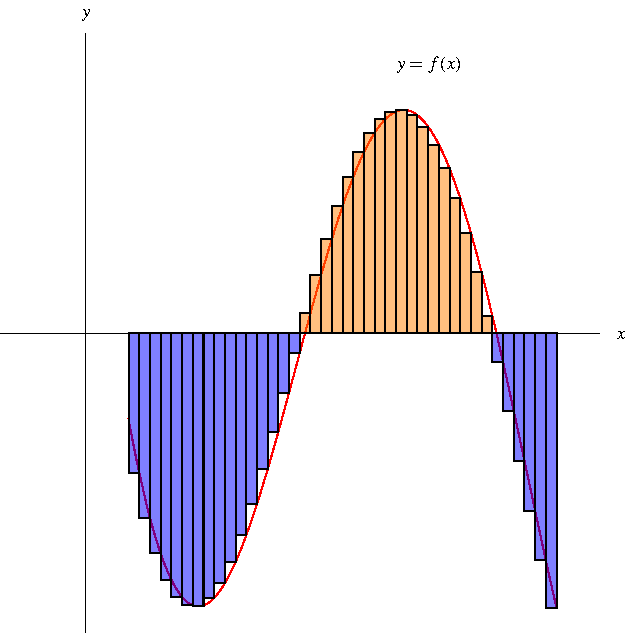
\includegraphics[height=4.2cm]{integration/pictures/05-02-net-areah.pdf}%
%}%
%\only<handout:1| 19->{%
%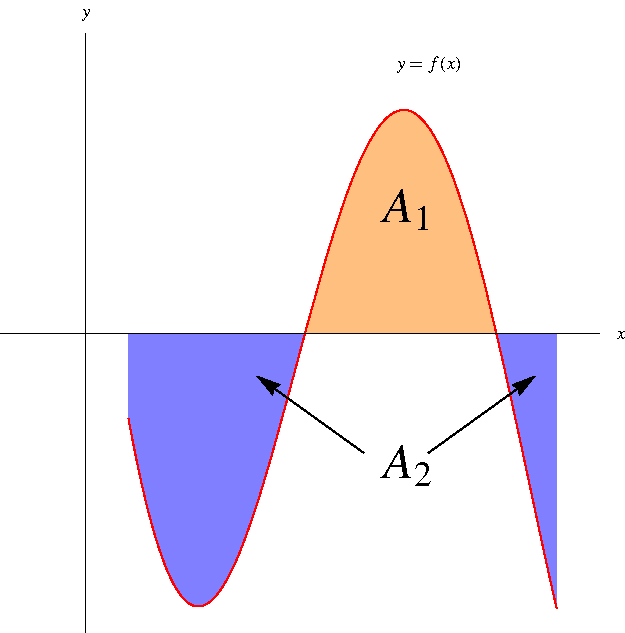
\includegraphics[height=4.2cm]{integration/pictures/05-02-net-area-limit.pdf}%
%}%
}%
\column{.6\textwidth}
\begin{itemize}
\item<10->  What if $f(x)$ is sometimes negative?
\uncover<handout:2|19->{
\item<19->  Then $\int_a^bf(x)\diff x = A_1 - A_2$.
\item<19->  $A_1$ is the area of the region above the $x$-axis and below the graph of $f$.
\item<19->  $A_2$ is the area of the region below the $x$-axis and above the graph of $f$.
}
\end{itemize}
\end{columns}
\end{frame}
% end module definite-integral-negative

%% begin module summation-formulas
\begin{frame}
The following formulas can be used to evaluate integrals.
\begin{align*}
\sum_{i=1}^n i & =  \frac{n(n+1)}{2}\\
\sum_{i=1}^n i^2 & =  \frac{n(n+1)(2n+1)}{6}\\
\sum_{i=1}^n i^3 & =  \left[\frac{n(n+1)}{2}\right]^2\\
\sum_{i=1}^n c & =  nc\\
\sum_{i=1}^n ca_i & =  c\sum_{i=1}^n a_i\\
\sum_{i=1}^n (a_i+b_i) & =  \sum_{i=1}^n a_i + \sum_{i=1}^n b_i
\end{align*}
\end{frame}
% end module summation-formulas

%% begin module definite-integral-ex2
\begin{frame}
\begin{example}
\begin{columns}
\column{0.15\textwidth}
\psset{xunit=0.2cm, yunit=0.2cm}
\begin{pspicture}(-0.5,-0.5)(3.1,9.1)
\fcBoundingBox{-1}{-7}{4}{9}
\pscustom*[linecolor=\fcColorNegativeAreaUnderGraph]{
%Function formula: x^{3}-6 x 
\psplot{0}{6 sqrt}{x -6 mul x 3 exp add }\psline(! 6 sqrt 2 1.5 exp 6 sqrt 6 mul sub)(! 6 sqrt  0)}
\pscustom*[linecolor=\fcColorAreaUnderGraph]{
%Function formula: x^{3}-6 x 
\psplot{6 sqrt}{3}{x -6 mul x 3 exp add }\psline(3, 9)(3,  0)}
\fcAxesStandardNoFrame{-1}{-7}{4}{9}
%Function formula: x^{3}-6 x 
\psplot[linecolor=\fcColorGraph, plotpoints=1000]{0}{3}{x -6 mul x 3 exp add }
\end{pspicture}
\column{0.85\textwidth}
Evaluate $\int_0^3 (x^3 - 6x)\diff x$. \uncover<2->{\alert<handout:0| 2-3,6>{ $\Delta x = \frac{b-a}{n} = \uncover<3->{\frac{3}{n}.}$}}

\abovedisplayskip=0pt
\belowdisplayskip=0pt
\abovedisplayshortskip=0pt
\belowdisplayshortskip=0pt
\begin{align*}
&\invisible{=}  \uncover<4->{%
\int_0^3 (x^3-6x)\diff x%
}%
\uncover<4->{%
 =  \lim_{n\to\infty} \sum_{i=1}^n f(\alert<handout:0| 7-8>{x_i})\alert<handout:0| 5-6>{\Delta x}%
}%
\uncover<5->{%
 = \lim_{n\to\infty} \sum_{i=1}^n f\left(\uncover<8->{\alert<handout:0| 8>{\frac{3i}{n}}}\right)\uncover<6->{\alert<handout:0| 6>{\frac{3}{n}}}%
}\\%
 & \uncover<9->{ = }  \uncover<9->{%
\lim_{n\to\infty} \frac{3}{n}\sum_{i=1}^n \left[ \left(\frac{3i}{n}\right)^3 - 6\left(\frac{3i}{n}\right)\right]%
}%
\uncover<10->{%
  =  \lim_{n\to\infty} \frac{3}{n}\sum_{i=1}^n \left[ \frac{27}{n^3}i^3 - \frac{18}{n}i\right]%
}\\%
 & \uncover<11->{ = }  \uncover<11->{%
\lim_{n\to\infty} \left[ \frac{81}{n^4}\alert<handout:0| 12-13>{\sum_{i=1}^n i^3} - \frac{54}{n^2} \alert<handout:0| 14-15>{\sum_{i=1}^n i}\right]%
}\\%
 & \uncover<12->{ = }  \uncover<12->{%
\lim_{n\to\infty} \left( \frac{81}{n^4}\uncover<13->{\alert<handout:0| 13>{\left[ \frac{n(n+1)}{2}\right]^2}} - \frac{54}{n^2} \uncover<15->{\alert<handout:0| 15>{\frac{n(n+1)}{2}}}\right)%
}\\%
 & \uncover<16->{ = }  \uncover<16->{%
\lim_{n\to\infty} \left[ \frac{81}{4}\left( 1 + \frac{1}{n}\right)^2 - 27 \left( 1 + \frac{1}{n}\right) \right]%
}%
\uncover<17->{%
 = \frac{81}{4} - 27 = -\frac{27}{4}
}%
\end{align*}
\end{columns}

\end{example}
\end{frame}
% end module definite-integral-ex2

% WARNING: This next module could use some pictures.
%% begin module definite-integral-properties
\begin{frame}
\frametitle{Properties of the Definite Integral}
\begin{itemize}
\item  So far when we have calculated $\int_a^b f(x)\diff x$, we have assumed that $a < b$.
\item  The definition as a limit of Riemann sums will still work even if we don't assume this.
\item<2->  If we reverse $a$ and $b$, then $\Delta x$ changes from $\frac{b-a}{n}$ to $\frac{a-b}{n}$.
\end{itemize}
\[
\uncover<3->{%
\alert<handout:0| 3-4>{%
\int_b^a f(x)\diff x = %
}%
}%
\uncover<4->{%
\alert<handout:0| 3-4>{%
- \int_a^b f(x)\diff x %
}%
}%
\]
\begin{itemize}
\item<5-| alert@5-6>  If $a = b$, then $\Delta x = $ \uncover<6->{$0$.}
\end{itemize}
\[
\uncover<7->{%
\alert<handout:0| 7-8>{%
\int_a^a f(x) \diff x = %
}%
}%
\uncover<8->{%
\alert<handout:0| 7-8>{%
0 %
}%
}%
\]
\end{frame}

\begin{frame}
Properties of the Integral
\begin{enumerate}
\item<1-| alert@2>  $\int_a^b c\diff x = c(b-a)$, where $c$ is any constant.
\item<1-| alert@3>  $\int_a^b [f(x)+g(x)] \diff x = \int_a^b f(x)\diff x + \int_a^b g(x) \diff x$.
\item<1-| alert@4>  $\int_a^b cf(x) \diff x = c\int_a^b f(x)\diff x$, where $c$ is any constant.
\item<1-| alert@5>  $\int_a^b [f(x)-g(x)] \diff x = \int_a^b f(x)\diff x - \int_a^b g(x) \diff x$.
\end{enumerate}
\end{frame}
% end module definite-integral-properties

%% begin module definite-integral-properties-ex6
\begin{frame}
\begin{example}[Example 6, p. 308]
Use the properties of integrals to evaluate
\begin{eqnarray*}
\alert<handout:0| 2-3>{\int_0^1 (4+3x^2)\diff x }%
& \uncover<2->{ = } &%
\uncover<2->{%
\alert<handout:0| 2-3>{\int_0^1 4\diff x + \int_0^1 \alert<handout:0| 4-5>{3}x^2\diff x \qquad \textrm{Property} \ \uncover<3->{2}}%
}\\%
& \uncover<4->{ = } &%
\uncover<4->{%
\alert<handout:0| 6-8>{\int_0^1 4\diff x} + \alert<handout:0| 4-5>{3}\int_0^1 x^2\diff x \qquad \alert<handout:0| 4-5>{\textrm{Property} \ \uncover<5->{3}}%
}\\%
& \uncover<6->{ = } &%
\uncover<6->{%
\alert<handout:0| 6-8>{\uncover<7->{4(1-0)}} + 3\alert<handout:0| 9-10>{\int_0^1 x^2\diff x} \qquad \alert<handout:0| 6-8>{\textrm{Property} \ \uncover<8->{1}}%
}\\%
& \uncover<9->{ = } &%
\uncover<9->{%
4 + 3\cdot \alert<handout:0| 9-10>{\uncover<10->{\frac{1}{3}}} \qquad \alert<handout:0| 10>{\uncover<10->{\textrm{Example 1, p. 289}}}%
}\\%
& \uncover<11->{ = } &%
\uncover<11->{%
5%
}%
\end{eqnarray*}
\end{example}
\end{frame}
% end module definite-integral-properties-ex6

% WARNING: This next module could use some pictures.
%% begin module definite-integral-properties-split
\begin{frame}[t]
Properties of the Integral
\begin{enumerate}
\setcounter{enumi}{4}
\item  $\displaystyle %
\alertNoH{ 1}{\int_a^b f(x) \diff x} %
= %
\alertNoH{ 2}{\int_a^c f(x) \diff x} %
+ %
\alertNoH{ 3}{\int_c^b f(x) \diff x} %
$%
\end{enumerate}
\begin{center}
\psset{xunit=1.5cm, yunit=1.5cm}
\begin{pspicture}(-0.5,-0.5)(4.5,3.6)
\psframe*[linecolor=white](-0.5,-0.5)(4.5,3.6)
%Function formula: 1727/6250+4911/100 ((x)^{3})+110043/5000 (x)+3 ((x)^{5})-201/10 ((x)^{4})-52431/1000 ((x)^{2})
\uncover<1>{
\pscustom*[linecolor=\fcColorAreaUnderGraph]{
\psplot[linecolor=red, plotpoints=1000]{0.1}{2.5}{x 2 exp -52.431 mul x 4 exp -20.1 mul x 5 exp 3 mul x 22.0086 mul x 3 exp 49.11 mul 0.27632 add add add add add }
\psline(2.5, 0)(0.1,0)
}
}
\uncover<2>{
\pscustom*[linecolor=\fcColorAreaUnderGraph]{
\psplot[linecolor=red, plotpoints=1000]{0.1}{1.7}{x 2 exp -52.431 mul x 4 exp -20.1 mul x 5 exp 3 mul x 22.0086 mul x 3 exp 49.11 mul 0.27632 add add add add add }
\psline(1.7, 0)(0.1,0)
}
}
\uncover<3>{
\pscustom*[linecolor=\fcColorAreaUnderGraph]{
\psplot[linecolor=red, plotpoints=1000]{1.7}{2.5}{x 2 exp -52.431 mul x 4 exp -20.1 mul x 5 exp 3 mul x 22.0086 mul x 3 exp 49.11 mul 0.27632 add add add add add }
\psline(2.5, 0)(1.7,0)
}
}

\psline(0.1, 0.05)(0.1, -0.05)
\rput[t](0.1, -0.07){$a$}
\psline(1.7, 0.05)(1.7, -0.05)
\rput[t](1.7, -0.07){$c$}
\psline(2.5, 0.05)(2.5, -0.05)
\rput[t](2.5, -0.07){$b$}
\rput(1.5, 2.4 ){$y=f(x)$}
\psaxes[ticks=none, labels=none]{<->}(0,0)(-0.5,-0.5)(4,2.7)\tiny
\psplot[linecolor=red, plotpoints=1000]{0.1}{2.5}{x 2 exp -52.431 mul x 4 exp -20.1 mul x 5 exp 3 mul x 22.0086 mul x 3 exp 49.11 mul 0.27632 add add add add add }
\end{pspicture}
%\only<handout:0| -1>{%
%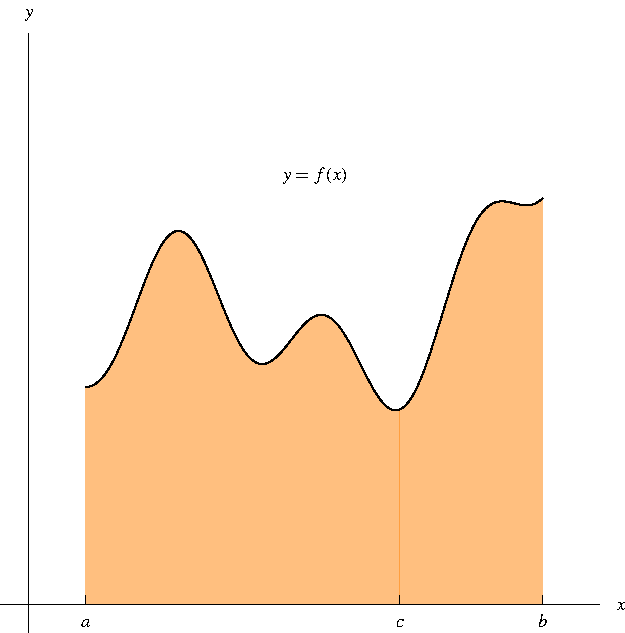
\includegraphics[height=5.6cm]{integration/pictures/05-02-splita.pdf}%
%}%
%\only<handout:0| 2>{%
%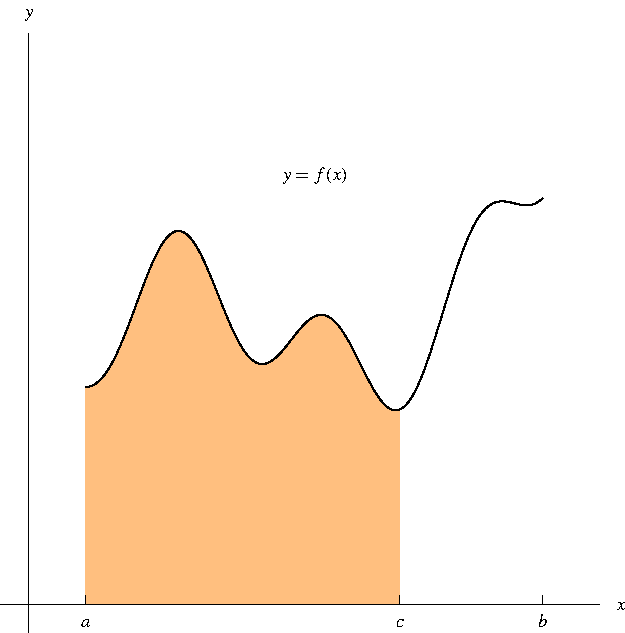
\includegraphics[height=5.6cm]{integration/pictures/05-02-splitb.pdf}%
%}%
%\only<handout:0| 3>{%
%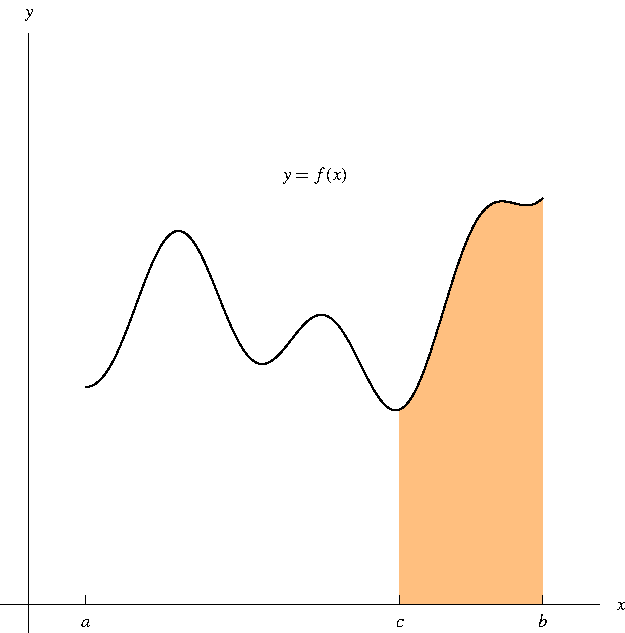
\includegraphics[height=5.6cm]{integration/pictures/05-02-splitc.pdf}%
%}%
\end{center}
\end{frame}
% end module definite-integral-properties-split

%% begin module definite-integral-properties-ex7
\begin{frame}
\begin{example} %[Example 7, p. 352]
If it is known that \alert<handout:0| 5-6>{$\int_0^{10}f(x)\diff x = 17$} and \alert<handout:0| 7-8>{$\int_0^8 f(x) \diff x = 12$}, then find $\int_8^{10}f(x) \diff x$.
\abovedisplayskip=0pt
\belowdisplayskip=0pt
\abovedisplayshortskip=0pt
\belowdisplayshortskip=0pt
\begin{align*}
\uncover<2->{%
\int_{\alert<handout:0| 2-3>{0}}^{\alert<handout:0| 2-3>{8}} f(x)\diff x + \int_{\alert<handout:0| 2-3>{8}}^{\alert<handout:0| 2-3>{10}}f(x)\diff x%
}%
& \uncover<3->{ = } %
\uncover<3->{%
\int_{\alert<handout:0| 3>{0}}^{\alert<handout:0| 3>{10}}f(x)\diff x%
}\\%
\uncover<4->{%
\int_{\alert<handout:0| 2-3>{8}}^{\alert<handout:0| 2-3>{10}}f(x)\diff x%
}%
& \uncover<4->{ = } %
\uncover<4->{%
\alert<handout:0| 5-6>{\int_{\alert<handout:0| 3>{0}}^{\alert<handout:0| 3>{10}}f(x)\diff x} - \alert<handout:0| 7-8>{\int_{\alert<handout:0| 2-3>{0}}^{\alert<handout:0| 2-3>{8}} f(x)\diff x}%
}\\%
& \uncover<5->{ = } %
\uncover<5->{%
\alert<handout:0| 5-6>{\uncover<6->{17}} - \alert<handout:0| 7-8>{\uncover<8->{12}}%
}\\%
& \uncover<9->{ = } %
\uncover<9->{%
5%
}%
\end{align*}
\end{example}
\end{frame}
% end module definite-integral-properties-ex7

% WARNING: This next module could use some pictures.
%% begin module definite-integral-properties-comparison
\begin{frame}[t]
Comparison Properties of the Integral
\begin{enumerate}
\setcounter{enumi}{5}
\item  If $f(x)\geq 0$ for all $a\leq x \leq b$, then $\displaystyle \int_{a}^{b} f(x)\diff x \geq 0$.
\end{enumerate}
\end{frame}

\begin{frame}[t]
Comparison Properties of the Integral
\begin{enumerate}
\setcounter{enumi}{6}
\item  If $f(x)\leq g(x)$ for all $a\leq x \leq b$, then $\displaystyle \int_{a}^{b} f(x)\diff x \leq \int_{a}^{b} g(x)\diff x$.
\end{enumerate}
\begin{center}
\psset{xunit=0.9cm, yunit=0.9cm}
\begin{pspicture}(-0.5,-0.5)(6,4.5)
\psframe*[linecolor=white](-0.5,-0.5)(6,4.5)
\tiny
\rput[l](5.1, 2.6){$y=g(x)$}
\rput[l](5.1, 1.3){$y=f(x)$}
\uncover<2>{
\pscustom*[linecolor=cyan]{
\psplot[linecolor=red, plotpoints=1000]{0.2}{5}{x 2 exp -0.18 mul x 3 exp 0.025 mul x 0.368 mul 0.808 add add add }
\psline(5,0)(0.2,0)
}
}
\uncover<3->{
\pscustom*[linecolor=cyan]{
\psplot[linecolor=red, plotpoints=1000]{0.2}{5}{x -9.9495 mul x 3 exp -2.0625 mul x 4 exp 0.1875 mul x 2 exp 7.4925 mul 5.6936 add add add add }
\psline(5,0)(0.2,0)
}
}
%Function formula: 101/125+46/125 (x)+1/40 ((x)^{3})-9/50 ((x)^{2})
\psplot[linecolor=red, plotpoints=1000]{0.2}{5}{x 2 exp -0.18 mul x 3 exp 0.025 mul x 0.368 mul 0.808 add add add }
%Function formula: 7117/1250+2997/400 ((x)^{2})+3/16 ((x)^{4})-33/16 ((x)^{3})-19899/2000 (x)
\psaxes[ticks=none, labels=none]{<->}(0,0)(-0.5,-0.5)(6,4.5)
\psplot[linecolor=red, plotpoints=1000]{0.2}{5}{x -9.9495 mul x 3 exp -2.0625 mul x 4 exp 0.1875 mul x 2 exp 7.4925 mul 5.6936 add add add add }
\psline(0.2, -0.1)(0.2, 0.1)
\rput[t](0.2, -0.15){$a$}
\psline(5, -0.1)(5, 0.1)
\rput[t](5, -0.15){$b$}
\end{pspicture}
%\only<handout:0| -1>{%
%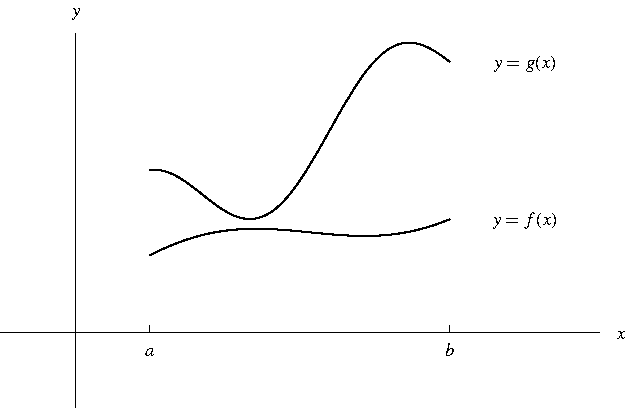
\includegraphics[height=4.2cm]{integration/pictures/05-02-comparisona.pdf}%
%}%
%\only<handout:0| 2>{%
%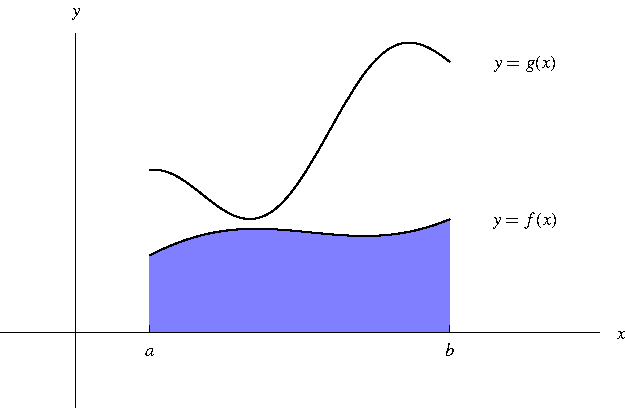
\includegraphics[height=4.2cm]{integration/pictures/05-02-comparisonb.pdf}%
%}%
%\only<handout:0| 3>{%
%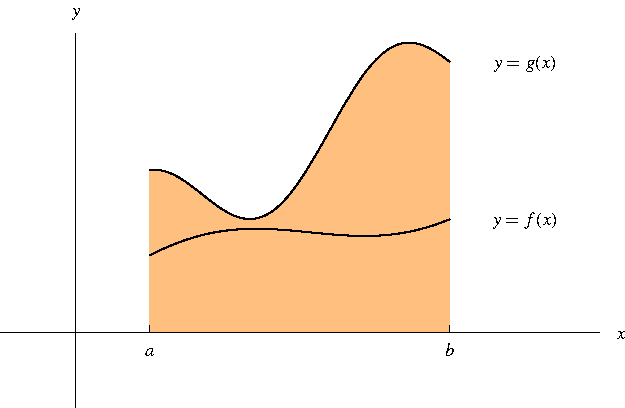
\includegraphics[height=4.2cm]{integration/pictures/05-02-comparisonc.pdf}%
%}%
\[
\alertNoH{ 2}{\int_a^b f(x) \diff x}%
 \leq  %
\alertNoH{ 3}{\int_a^b g(x) \diff x}%
\]
\end{center}
\end{frame}

\begin{frame}[t]
Comparison Properties of the Integral
\begin{enumerate}
\setcounter{enumi}{7}
\item  If $m\leq f(x)\leq M$ for all $a\leq x \leq b$, then
\[
\alertNoH{ 2}{m(b-a)}%
 \leq  %
\alertNoH{ 3}{\int_a^b f(x) \diff x}%
 \leq  %
\alertNoH{ 4}{M(b-a)}%
\]
\end{enumerate}
\begin{center}
\psset{xunit=0.9cm, yunit=0.9cm}
\begin{pspicture}(-0.5,-0.5)(6,4.5)
\psframe*[linecolor=white](-0.5,-0.5)(6,4.5)
\tiny
\uncover<2>{
\pscustom*[linecolor=orange]{
\psplot[linecolor=\fcColorGraph, plotpoints=1000]{0.2}{5}{0.7}
\psline(5,0)(0.2,0)
}
}

\uncover<3>{
\pscustom*[linecolor=cyan!50]{
\psplot[linecolor=\fcColorGraph, plotpoints=1000]{0.2}{5}{x -9.9495 mul x 3 exp -2.0625 mul x 4 exp 0.1875 mul x 2 exp 7.4925 mul 5.6936 add add add add }
\psline(5,0)(0.2,0)
}
}
\uncover<4>{
\pscustom*[linecolor=cyan]{
\psplot[linecolor=red, plotpoints=1000]{0.2}{5}{4.3}
\psline(5,0)(0.2,0)
}
}
%Function formula: 7117/1250+2997/400 ((x)^{2})+3/16 ((x)^{4})-33/16 ((x)^{3})-19899/2000 (x)
\psaxes[ticks=none, labels=none]{<->}(0,0)(-0.5,-0.5)(6,4.5)
\psplot[linecolor=\fcColorGraph, plotpoints=1000]{0.2}{5}{x -9.9495 mul x 3 exp -2.0625 mul x 4 exp 0.1875 mul x 2 exp 7.4925 mul 5.6936 add add add add }
\psline[linecolor=\fcColorGraph](0.2, 0.7)(5,0.7)
\psline[linecolor=\fcColorGraph](0.2, 4.3)(5, 4.3)


\rput[r](4.9, 2.6){\alertNoH{3}{$y=f(x)$}}
\psline[linestyle=dotted, arrows=<->](5.05, 0)(5.05, 0.7)
\rput[l](5.15,0.35){\alertNoH{2}{$m$}}
\psline[linestyle=dotted, arrows=<->](5.5, 0)(5.5, 4.3)
\rput[l](5.6,2.15){\alertNoH{4}{$M$}}

\psline(0.2, -0.1)(0.2, 0.1)
\rput[t](0.2, -0.15){\alertNoH{2,4}{$a$}}
\psline(5, -0.1)(5, 0.1)
\rput[t](5, -0.15){\alertNoH{2,4}{$b$}}
\end{pspicture}
%\only<handout:0| -1>{%
%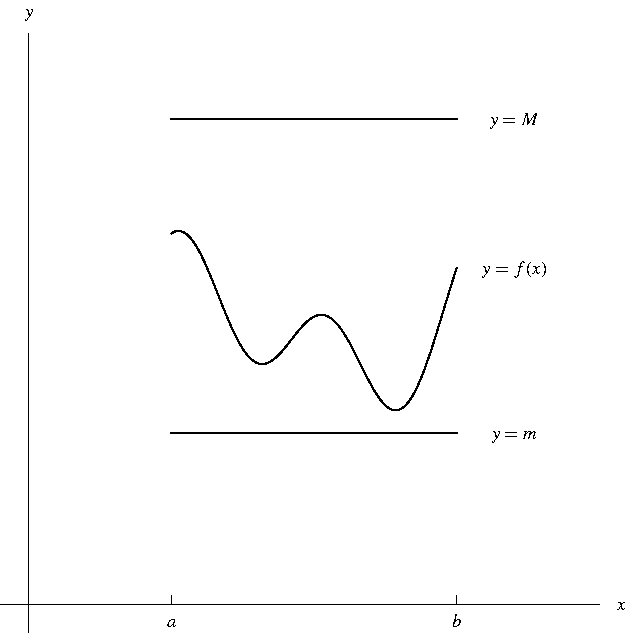
\includegraphics[height=5.6cm]{integration/pictures/05-02-boundinga.pdf}%
%}%
%\only<handout:0| 2>{%
%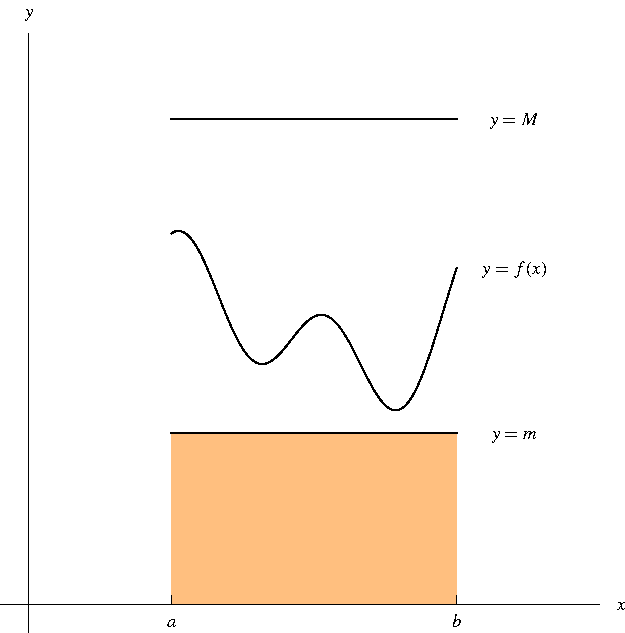
\includegraphics[height=5.6cm]{integration/pictures/05-02-boundingb.pdf}%
%}%
%\only<handout:0| 3>{%
%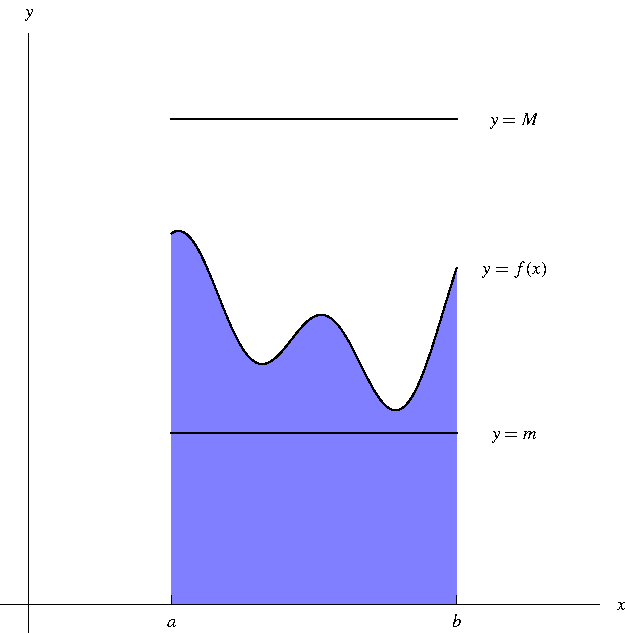
\includegraphics[height=5.6cm]{integration/pictures/05-02-boundingc.pdf}%
%}%
%\only<handout:0| 4>{%
%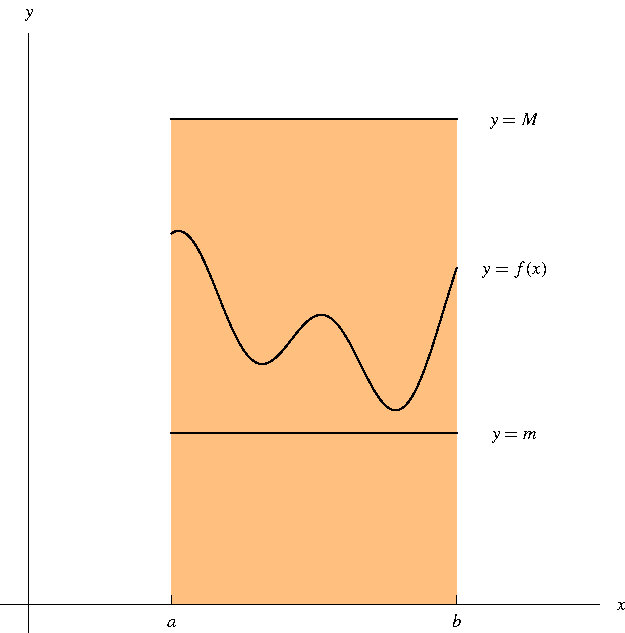
\includegraphics[height=5.6cm]{integration/pictures/05-02-boundingd.pdf}%
%}%
\end{center}
\end{frame}
% end module definite-integral-properties-comparison


\end{document}
